\documentclass{aifyp}

\usepackage[numbers]{natbib}

% Change the placeholder 999 below to the widest number you need 
\renewcommand\bibnumfmt[1]{\hphantom{[0]}\llap{[#1]}}

\usepackage{url}
\usepackage{acronym}
\usepackage{pdfpages}
\usepackage[normalem]{ulem}
\useunder{\uline}{\ul}{}
\usepackage{siunitx}
\usepackage{blkarray}
\usepackage{amsmath}
\usepackage[toc,page]{appendix}
\usepackage{subfig}
\usepackage{graphicx}
\usepackage{blindtext}
\usepackage{float}
\usepackage[bottom]{footmisc}
\usepackage[section]{placeins}
\usepackage{etoolbox}
\AtBeginEnvironment{quote}{\singlespacing\small}
\raggedbottom

\title{Workplace Assistant Augmented Reality}
\author{Gabriel Camilleri}
\supervisor{Dr. Vanessa Camilleri}
\date{May 2020}
\acknowledgement{The research work disclosed in this publication is partially funded by the Department of Artificial Intelligence. \emph{}}

\longabstract{
\indent Starting a new job in an office can be very stressful for an intern or a new employee, especially on their first day at the office. It takes time to adjust and learn what other employees’ jobs are and how they can be beneficial to them. It might additionally take some time for new members to learn the ropes and their purpose within the office building, while understanding and learning how to use certain equipment, for example, an automatic key lock or simply a coffee machine. Therefore, the Workplace Assistant Augmented Reality tries to identify the user's requirements in accomplishing a specific task within the workplace through user profiling and recommendation, whilst providing the relevant information for the user to learn and understand the environment around them via augmented reality.
  \newline
  \newline
\indent The application is intended to guide new employees through an adapted process which enables them to understand the environment around them along with equipment which they might use daily. It will also be intended on guiding the users, providing them with relevant information in order to successfully accomplish their task. The system incorporates collaborative filtering and a similarity-based technique using SVD++ and item to item based similarity respectively, to provide recommendations, along with deep learning and traditional computer vision techniques using Vuforia, to provide augmented reality. Using the tools mentioned the system provides information about offices, directions towards specific offices, and information on how to utilise the coffee machine of the company which the application was tailor made for.
\newline
\newline
\indent From the tests performed the indication is that the SVD++ model was the most efficient model to apply in comparison to other machine learning models, when applied with AR. The model achieved average Root Mean Square Error and Mean Absolute Error of 3.1226 and 2.6866, respectively. The AR component achieved promising distance, colour, rotation and occlusion variance values. Finally, the system obtained on average positive qualitative results via user-feedback along with recommendations on how it may be further improved. 

}

\acknowledgement{
I would firstly like to thank my supervisor Dr.Vanessa Camilleri for her constant feedback and help provided during this Final Year Project. Secondly, I would also like to thank CCBill, for allowing me to carry out my research for WAAR on their behalf using their environment as a basis for my application.
}


\begin{document}
\pagenumbering{roman} 
\tableofcontents
\clearpage{\pagestyle{empty}}

\section*{Acronyms}
\begin{acronym}
\acro{WAAR} {Workplace Assistant Augmented Reality}
\acro{AR} {Augmented Reality}
\acro{SIFT}{Scale-invariant feature transform}
\acro{SURF}{Speeded Up Robust Features}
\acro{RSS}{Received Signal Strength}
\acro{HMD}{Head Mounted Display}
\acro{MAR}{Mobile Augmented Reality}
\acro{CV}{Computer Vision}
\acro{BRIEF}{Binary Robust Independent Elementary Features}
\acro{FAST}{Features from Accelerated Segment Test}
\acro{CNN}{Convolution Neural Network}
\acro{HIT}{Hyperlink-Induced Topic Search}
\acro{OJT}{On the Job Training}
\acro{AMT}{Aircraft Maintenance Technician}
\acro{SVD++/SVDpp}{Singular Value Decomposition Plus Plus}
\acro{SDK}{Software Development Kit}
\acro{TF}{Term Frequency}
\acro{TFIDF}{Term Frequency Inverse Document Frequency}
\acro{PCA}{Principal Component Analysis}
\acro{RMSE}{Root Mean Square Error}
\acro{MAE}{Mean Absolute Error}
\acro{SUS}{System Usability Scale}
\end{acronym}
\newpage
\listoffigures
\clearpage{\pagestyle{empty}}

\listoftables
\clearpage{\pagestyle{empty}}



\pagenumbering{arabic} 
\setcounter{page}{1}



\section{Introduction}
\label{s:intro}
\subsection{Problem Definition}
\indent Starting a new job in an office can be very stressful for an intern or a new employee, especially on their first day at the office. It takes time to adjust and learn what other employees’ jobs are and how they can be beneficial to them. It might additionally take some time for new members to learn the ropes and their purpose within the office building, while understanding and learning how to use certain equipment, for example, an automatic key lock or simply a coffee machine. ``Person-job fit is a substantial factor for decreasing job stress and the adjustment of employees to an organization is an important issue for eliminating stress”\cite{DENIZ2015369}.
% ``New employees all bring expectations to their new jobs that are based on factors like their previous job experiences, their understandings of the profession, beliefs and experiences held by peers or family, promises made during recruitment, and their evaluation of the work situation during their interview”\cite{MOITA8S}. 
In a research carried out by  P. Moita \cite{MOITA8S}, is discussed how new employees start a new job with high expectations due to several factors such as previous jobs or promises made during recruitment. The first month at the workplace might seem overwhelming for new employees. Therefore, during their first few months of settling and adjusting, the company may allow ``a period of learning how to ‘fit in’ and adjusting to how things work in the new setting”\cite{MOITA8S} for the employee’s benefit.
\newline
\newline
\indent Providing an assistant AR application to help speed up the process for the employee to adjust to their new workplace environment may offer several challenges. There are several AR libraries which provide all the necessary techniques for one to build such applications. However using algorithms, techniques, and models which involve A.I, may help in overcoming those challenges in image and object recognition. 
% When it comes to feature extraction, things can be challenging, especially if one is making use of traditional computer vision techniques, such as, SIFT and SURF alone. For instance, 
For instance, ``[t]he SIFT algorithm deals with the problem that certain image features like edges and corners are not scale-invariant. In other words, there are times when a corner looks like a corner but looks like a completely different item when the image is blown up by a few factors”\cite{Lee2016ComparingDN}. Therefore one can combine the algorithms mentioned with deep learning techniques to allow the application to recognise real world objects as efficiently as possible,without hindering the user's experience. 

\subsection{Motivation}
% \indent “Whilst employees can be reasonably expected to adjust to changes in jobs over time, poor job or employee job fit can result in increased stress and inefficiency in organizations”
As discussed in the following research by N. Deniz \cite{DENIZ2015369}, poor employee-job fitness can result in poor performances within the workplace. Adjusting to a new environment, especially one’s workplace, can come with several challenges, such as, adapting to new people, finding certain offices within the environment, and using certain job equipment. ``When humans feel a loss of control this causes physiological changes which can exacerbate feelings of stress”\cite{DENIZ2015369}. Job stress has become a common term in industry since several companies endeavour to sustain a healthy working environment for their employees. As discussed by N. Barzegar and S. Farjad in their research \cite{VIJAYANMATHANGI2}, job stress along with workload has been one of the major causes that affect employees' productivity and efficiency.
\newline
\newline
\indent Such level of stress can increase from certain necessary adjustments for the employee to settle within a company, such as, filling in papers and handing them to the right offices, and learning to use certain equipment around them. Therefore, proper training should always be provided, whether it is detailed or otherwise. ``Application of training in the workplace and proper implementation of training can directly lead to improving the employees' performance”\cite{BARZEGAR20111942}.
\newline
\newline
\indent There are two types of training, namely, on the job and off the job training. On the job training is a method of imparting knowledge and training directly while on the job. Conversely, off the job training is a method of imparting knowledge and training while not at the place of work, for example, through a site. The idea behind training is to minimise stress levels and allow the employee to improve without any pressure. As stated by Barzegar and S. Farjad in their research, ``Training, which aims at empowerment, development, and qualifying employees through knowledge and skills, refers to end-oriented, organized, logical, on-going planned attempts to bring about the desired change in the knowledge, skills, capability and attitude of employees” \cite{BARZEGAR20111942}.

\subsection{Why the Problem is Non-Trivial}
\indent There have been previous attempts at making indoor AR applications to guide users around a place. However, most attempts are usually made using ArCore and acquiring a 3D model of the building or using an indoor positioning syst. ArCore is useful for catching movements and current positioning, as well as light detection. It further has the anchoring feature where a virtual object is given a marker to monitor its displacement. However, ArCore is incompatible with several devices, and it would thus be futile to apply it in real-life scenarios since not everyone will have the latest phone with the latest specs. Vuforia, on the other hand, is more user-friendly and can be used on several operating systems.
\newline
\newline
\indent The second problem is that the AR application can be fed a 3D model directly to anchor positions within the map and display the respective augmented information. This can be useful when applying smart indoor AR navigation. However, creating a 3D model of the workplace can have several problems. Firstly, the company would not want to hand out freely a plot of its indoor workplace as this goes against its policy. Secondly, one would not be testing and experimenting with anything if a 3D model of the workplace were used. In this project, several features will be tested from Vuforia’s library, such as, feature detection, and the library will be used to its full potential.

\subsection{Approach}
\indent The proposed solution is to develop a workplace assistant augmented reality (WAAR) application to assist users by providing them with AR information to guide them to offices, provide them with information about offices and rooms while walking down the corridor, and give instructions on how to use the office coffee machine. The application will make use of user profiling techniques to understand users’ requirements, and will display relevant information related to the purpose for using the application. It will be necessary for the user to make some initial choices of interest to provide recommendation and profiling techniques to, in this case this may be the task one is interested in accomplishing (Interview, Delivery, and Visit) for the visitors side, whereas for the interns side, direct offices of interest which they are required to find as well as choosing secondary places which may interest them (i.e gamesroom, restrooms, and kitchen room). 
\newline
\newline
\indent AR development will be handled by Vuforia’s libraries since Vuforia has some features which the application can well benefit from. For our research, image and object segmentation and recognition will be used to identify office workplace markers along with Unity(to build the application's architecture), and the proper content will be overlaid using game objects. There will be instances where model target and Vuforia’s deep learning techniques are used to scan some objects in 3D. Vuforia is ideal because it can develop AR applications for Android and IOS devices.
\newline
\newline
\indent Indoor navigation can be done in several ways. One can use GPS signals, beacons, RSS or WIFI signals, or simply AR itself. Furthermore, AR can be either location-based or marker-based. Therefore, the proposed solution for our problem is to use AR marker-based navigation by using several markers around the office building to segment images or objects, while displaying the proper directions by recognising the markers in view thereby enabling the company to keep the application useful for offline use. For scenarios where WIFI or any other signals are down, users can still make good use of the application, for example, in case of an emergency to find the fire exit. 


\subsection{Aim and Objectives}
The aim of this project is to combine user profiling techniques with image and object detection and present these in an Augmented Reality application designed for the workplace.
\newline
\newline
The objectives of the final year project are:
\begin{itemize}
    \item Perform image and object detection techniques using the Vuforia Library;.
    \item Use AR techniques from the detected images and objects to overlay and augment information and navigation information.
    \item Develop user profiling techniques through a recommendation based system to filter out unnecessary information for augmentation.
    \item Apply and evaluate the developed and implemented artificially intelligent techniques through quality and quantity testing.
\end{itemize}

\subsection{Report Layout}
\indent The layout of the report is as follows. Chapter 2 provides background information about the technologies used. Subsequently, Chapter 3 includes the literature review which was conducted while attempting to solve the problem at hand. Chapter 4 is a brief overview of the system and its design.  Chapter 5 presents the implementation process, while Chapter 6 discusses the evaluation methods and approaches for the application, including both user and AI evaluation. The chapter further analyses the obtained results. Chapter 7 outlines the limitations encountered during the project, while offering recommendations for further development of the application and technologies used. Finally, the project is brought to an end with a conclusion in Chapter 8.
\pagebreak
\section{Background Research}
Besides providing some background research on the technologies applied in this project, this chapter will discuss thoroughly technical information about the workplace environment and applicable technologies in order to apply current AR technologies in such environments, while outlining any difficulties which might arise.
\subsection{User Profiling}
\indent As described by  S. Kanoje, D. Mukhopadhyay, and S. Girase, user profiling is a method which extracts information about the user via keywords and ``generate a structured Profile” \cite{KANOJE20165}. User profiling enables the system to tailor the required information for the user to see and use. It is rather annoying for users to have to go through irrelevant documents or data in an attempt to find information specific to what they require.
\newline
\newline
\indent ``User profile generation is done when we get user’s complete information while he registers into our system. We have identified different user attributes for profiling him into our system" \cite{KANOJE20165}.  User profiling has taken the form of recommender systems, thus providing user specific and personalised recommendations. There are two forms of user profiling. The first is Explicit User Profiling, which is an approach where the ``…user’s behaviour is predicted by analysing the user’s available data” \cite{Kanoje2015UserPT}. This is also known as Static Profiling, where static and predictable user data is analysed. The second type is Implicit User Profiling, which ``relies more on what we have known about user in future i.e. system tries to learn more about the user” \cite{Kanoje2015UserPT}. This type is also referred to as Adaptive Profiling. After performing extraction, one might end up with redundant information.
\newline
\newline
\indent To clean the information and see unique pieces of it, one must perform filtering. There are three filtering techniques for user profiling, namely, rule-based, collaborative, and content-based filtering. Rule-based filtering is the technique used to filter out content based on a set of rules, normally present using ``if-then” statements. Content-based filtering ``recommends items based on a comparison between the content of the items with a user profile and selects those items whose content best matches with the content of another item" \cite{Kanoje2015UserPT}. On the other hand, collaborative filtering is the process of grouping users with a similar search criterion. Filtering is based on previously sought items as well and items which one is more likely to search for next.
\pagebreak
\subsection{Augmented Reality}
\indent  As discussed by R. Silva, J. Oliveira, and G. Giraldi, ``Augmented Reality (AR) is a new technology that involves the overlay of computer graphics on the real world” \cite{IntoToAR}. It is a term which refers to mixed reality, where the digital world and reality are combined and interwoven. AR is a new form of technology that focuses on displaying realistic overlays on reality to provide extra information and content to what we see with our naked eyes.
% It is an enhanced version of a real-world environment, through the form of media devices such pictures, videos, 3D models and sounds. ``Therefore, AR can be differentiated from Virtual Reality, given that the former overlays digital information in a real environment, rather than completely replacing it.”\cite{CROFTON2019102178}.
\newline
\newline
\indent There are different categories of AR. The first category is marker-based AR, where the augmented overlay is only displayed once a marker is detected through a camera. It is also known as image recognition. The second category is markerless AR, which makes use of an accelerometer, GPS, and velocity tracker to detect the location of the phone and display the AR overlay in that specific location, given its location is predefined. The third category is projection-based, which basically projects data in the form of light rays on objects, for example, an augmented-projected keyboard. The last category is superimposed AR, where AR replaces partially the real view with an augmented one of the object. IKEA use this application in their digital catalogues.
\newline
\newline
\indent There are several AR devices. The first device is Optical See-Through HMD. ``Optical See-Through AR uses a transparent Head Mounted Display to show the virtual environment directly over the real world” \cite{IntoToAR}. HMD performs best when it fits perfectly to the users’ eyes and sits comfortable on their face, making it easy for them to move around when wearing it. The second type is Virtual Retinal Device, which ``...projects a modulated beam of light (from an electronic source) directly onto the retina of the eye producing a rasterized image” \cite{IntoToAR}. The third device is Video See-Through HMD, the monitor-based AR, which ``...uses merged video streams but the display is a more conventional desktop monitor or a handheld display” \cite{IntoToAR}. Finally, projection display, which projects on surfaces and is useful for multiple user interaction. One such example of projection-based AR is Tilt Five.

% \subsection{Vuforia}
% \indent Vuforia is the ``most popular SDK for developing AR-applications on a wide selection of devices"\cite{Grahn2017TheVS}. Similar to ARCore and ARKit, Vuforia can be used on multiple devices to recognise images, objects and text. One can use third party engines such as Unreal or Unity to display overlays to create Augmented Reality apps.
% \newline
% \newline
% \indent Image recognition works by detecting natural features such as edges and corners in an image. ``the feature tracking algorithm can determine what is a feature and map the positions of these features in the image" \cite{Grahn2017TheVS}. By shifting the positions of the image features like edges are intensified, even more corners as their position changes after shifting. Vuforia thus, makes use of Pose feature detection techniques where it takes into consideration the position and orientation of the natural features. It can make use of extended tracking, where the engine detects surrounding features as well. A proper image with high quality feature detection is an image that contains uniquely distinct features, which are not repetitive. For example, a dark circle is difficult to recognize and establish uniquely features.
% \newline
% \newline
% \indent Object Recognition in Vuforia works in several ways. The first method is by using a scanning plane which acts as an image target. Once it is recognised, it ``provides the scanner with the XYZ-coordinates of the detected features on the 3D object"\cite{Grahn2017TheVS}. The latest form of object detection is by using their latest release, modelling targets. They have added a new feature for target modelling using their own database on the cloud, where it contains multiple views and/or multiple objects with automatic recognition. It makes use of a deep learning library which is added as an SDK. One only needs to train a model target database where your 3D model is uploaded to the Cloud for training purposes. Text recognition in Vuforia makes use of Optical character recognition tools. The image cause through segmentation and the characters are extracted from the image background.

% \subsection{Human Computer Interaction Techniques and Methods}
% There are several approaches to Human computer interaction designing. Firstly, the Anthropomorphic Approach, which is the designing of a human like interface. Secondly is the Cognitive Approach, which takes into consideration cognitive abilities of the human for interfacing. Thirdly is the Empirical approach, which compares usability of multiple conceptual designs. This involves performing Human task performance measures and A/B Testing. Finally, the last approach is Predictive Modelling Approach. It is the examination of the amount of time the user took to complete a task using the interface provided.
% \newline
% \newline
% \indent There are eight research methods with respect to mobile HCI research. The first one is case studies. Case studies are intensive empirical studies using groups, organizations, individuals, systems or tools. Data is collected to qualitative and quantitative approaches. The second is Field studies, ``Ethnographic field studies are characterized by researchers spending significant amounts of time in the field and, to some extent, immersing themselves into the environment they study"\cite{KJJEGRCO}. Third one is Action research, fourth one is Laboratory Experiments where a controlled environment is used for research purpose, Fifth is survey research, sixth one is applied research where it ``builds on trial and error on the basis of the researchers capabilities of reasoning through intuition, experience, deduction and induction"\cite{KJJEGRCO}.The final two research method are basic research and normative writings.
\subsection{Mobile Augmented Reality}
Using AR on mobile devices presents several challenges which are ``related to context-awareness, usability, navigation, visualization and interaction design" \cite{IssuesMobileAR}. Handheld devices are nowadays equipped with powerful processors, cameras, and sensors. Smartphones use a ``camera on the opposite side of the display [which] encourages the use of the ‘magic lens’ metaphor describing the fact that the users have to point and look ‘through’ the device to view the augmented representation of the real world"\cite{IssuesMobileAR}. Although most cameras are equipped with high resolution, the screen and camera capture a limited range of field of view. Therefore, augmented information must clearly be placed on the smartphone screen and avoid obstructing the user from important views of the real world.
\newline
\newline
\indent A mobile AR framework is made up of three specific features \cite{phdthesisMobileAR}], namely, MAR Observer which obtains the target images or text from the AR server, MAR Server which ``serves as a bridge between the MAR customizer and MAR observer" \cite{phdthesisMobileAR}, and MAR application customizer which defines interactions between the user and image targets. In this case, Vuforia serves as the MAR application customizer.
\subsection{Augmented Reality Navigation}
Outdoor navigation usually makes use of GPS localisation. However, this can be a problem for indoor navigation. There are several ways to provide indoor localisation. One can use beams either by Bluetooth signals or WIFI signals thereby obtaining continuous mapping, albeit with rather irregular results at times. The alternative is to use offline waypoints, where the user simply scans a marker to get a location or augment pre-programmed information within that location. However, ``...the user needs to update his/her location by scanning another way-point on the way" \cite{Bhorkar2017ASO}.
\newline
\newline
\indent One main challenge of AR navigation is the process of registration, which ``...is the process of correctly aligning the virtual information with the real world in order to preserve the illusion of coexistence” \cite{Bhorkar2017ASO}. Although proper visual registrations must be met for the augmentation to be as realistic as possible, one must not forget that the user still needs to focus on what is in their path.
\newline
\newline
\indent Improvement of AR can help to provide navigational information without distracting the user to look away to a secondary screen or view by, “[f]or example, showing navigation markers on the windshield of the car or augmenting the video camera output of a smartphone with the navigation path” \cite{Bhorkar2017ASO}. To provide an AR navigation system there are several steps one needs to take, namely, “1. Acquire the real-world view from the user’s perspective. 2. Acquire the location information for tracking the user. 3. Generate the virtual world information based on the real-world view and the location information. 4. Register the virtual information generated with the real-world view” \cite{Bhorkar2017ASO}.

\subsection{Traditional Computer Vision for Object Detection}
Traditional CV is the “traditional approach…to use well-established CV techniques such as feature descriptors (SIFT, SURF, BRIEF, etc.) for object detection" \cite{ComputerVisVSDeep}. Images contain several features which can be extracted using CV algorithms, such as, edge detection, corner detection, and threshold segmentation for improved detection of such features. 
\newline
\newline
\indent Image recognition works by detecting natural features such as edges and corners in an image. “[T]he feature tracking algorithm can determine what is a feature and map the positions of these features in the image" \cite{VuforiaUnity}. By shifting the positions of the image, features like edges are intensified, with even more corners as their position changes after shifting. Therefore, Vuforia makes use of pose feature detection techniques, where it takes into consideration the position and orientation of the natural features. It can make use of extended tracking, where the engine detects surrounding features as well. A proper image with high quality feature detection is an image that contains uniquely distinct features which are not repetitive. For example, a dark circle is difficult to recognise and establish as a unique feature.
\newline
\newline
\indent As discussed in \cite{ComputerVisVSDeep}, it is up to the CV engineer to choose the correct and most important features which best classify an image, “[a]s the number of classes to classify increases, feature extraction becomes more and more cumbersome". 
% “The difficulty with this traditional approach is that it is necessary to choose which features are important in each given image. As the number of classes to classify increases, feature extraction becomes more and more cumbersome. It is up to the CV engineer’s judgment and a long trial and error process to decide which features best describe different classes of objects" \cite{ComputerVisVSDeep}. 
There are several advantages when using traditional CV techniques. SIFT and SURF algorithms are generally used for applications such as image stitching, where classes do not need to be identified within the image. Traditional techniques make use of less processing power, and the problem at hand is simple enough to use such traditional CV techniques with little amount of data needed, unlike a deep learning model.

\subsection{Deep Learning in Augmented Reality}
The detection problem has been solved using camera-based tracking systems to apply them to AR using deep learning techniques. The Vuforia Library has applied such techniques to scan 3D objects and create model targets for them in order to be easily recognisable within any developed AR app. This provides new advantages, such as, detectability from any angle of the recognisable real-world object. “Known model of the object can be used to determine the position and orientation of the object. Rendering of the virtual object follows easily” \cite{Akgul2016ApplyingDL}. There are two ways how the object can be recognised. One can use traditional artificial vision techniques, or Convolutional Neural Networks for improved detection.
\newline
\newline
\indent Model-based AR tracking is achievable in two steps. Firstly, one uses video tracking which “yields the pose of the camera with respect to the known target” \cite{Akgul2016ApplyingDL}. Secondly, the pose is sent to an algorithm for tracking. Such algorithms as SIFT \cite{SIFT} and SURF \cite{SURF} are commonly used for detection. The algorithm extracts a number of key points using a corner detection algorithm such as FAST \cite{CornerDetection}. In \cite{ Akgul2016ApplyingDL}, a CNN implementation was trained using AlexNet to detect patches. FAST was used to detect features on a reference image, extracting 15 by 15 patches across each feature. HIPS \cite{Taylor2011} was used for 8 by 8 sparse sampled patches from the original set of patches. When comparing the overall performance of the CNN used in \cite{Akgul2016ApplyingDL} with an algorithm such as ORB, the re-projection error shows that it was far improved in DeepAR. “DeepAR method produces consistently more inliers than HIPS. However, as can be seen in Figure 12 the percentage of inliers vs outliers are less for DeepAR” \cite{ Akgul2016ApplyingDL}.
\newline
\newline
\indent In their study, \cite{ Akgul2016ApplyingDL} concluded that “[t]he detector performance is very strong especially in the presence of error in feature localization” \cite{ Akgul2016ApplyingDL}. It is indeed comparable to one of the best feature detection algorithms to date.
\subsection{Conclusion}
This chapter provided and discussed background research and information on existing technologies and techniques which will be applied in FYP. The following chapter will present a literature review of the research published in the field of AR.
\newpage
\section{Literature Review}
\indent This chapter reviews the available literature on WAAR, while discussing the two components involved in the AR application and research that has inspired the approach selected for this project. The chapter is divided into three parts, namely, AR technologies involved with workplace assistance, the application of user profiling methods with AR, and different image and object recognition techniques in AR technologies.
\subsection{Workplace Augmented Reality}
\begin{quote}
[A]ugmented Reality (AR) technology has rarely been discussed outside  of the computer science world. It has taken years for this technology to become closer to a stable existence, and will most likely take several more years before it will be used by average citizens.\cite{ARInfoForWorkplace}
\end{quote}

\indent Although the technology can be considered still in its infancy, it also has a wide variety of applications. One of its main applications in the 4.0 Industry is the use of AR in assisted learning. Every workplace necessitates adjustment and some form of training for employees to adapt to the process of the work they might be doing. AR may assist employees by providing them with additional overlaid instructions to guide them through the whole process of adjustment while providing them with training.
\newline
\newline
\indent Workplace training is usually provided in two forms, namely, on the job training (OJT) and off the job training. “[O]JT may be viewed as an apprenticeship where a novice AMT is mentored by an AMT who is an expert” \cite{1563376}. This is the traditional form of training, especially when teaching maintenance. However, “[O]JT may not be the best method for training because the feedback to learners may be infrequent and unmethodical” \cite{1563376}. Conversely, off the job training may be provided through face to face conversations or through multimedia. AR can combine the two aspects of training, where the user is given on the job training through multimedia, which overlays the real-world environment.
\newline
\newline
\indent There are several useful applications for AR at the workplace. However, not every workplace might necessitate AR. “[T]here are situations where an AR system may be used to enhance the task completion process, or display and/or communication of information in conjunction with traditional technologies” \cite{ARInfoForWorkplace}. As discussed in \cite{ARInfoForWorkplace}, the following are workplace conditions where AR is applicable, namely, distance communication with 2D or 3D objects provided for visualisation, training and education when using real-life tools, recording of information obtained while training, and a collaborative design and interaction of 3D models.
\newline
\newline
\indent An advantage which AR offers to workers and managers is “[t]he ability to author their own environment by embedding the relevant information needed for task completion” \cite{ARInfoForWorkplace}. Nonetheless, a common problem during work training is that the expert individual needs to provide the respective information to the trainee in the most understandable way possible. Therefore, through AR technology, the trainee can tailor how that information is presented, and thus, AR may be capable of understanding its users such that it may adapt to future possible users.

\subsection{Recommendation Systems for Augmented Reality}
Information during job training is crucial for an employee to learn and adapt to the new environment. However, an overwhelming amount of information provided to a new employee may be demotivating. AR is a tool that provides interactive information to the user while also obtaining information from the user. Nevertheless, 
\begin{quote}...[t]he fact that the typical scene of these applications mix real and virtual elements can be a motivating factor for users. However, this feature may also make the interaction more complicated, which can affect the user experience in performing tasks within the application.\cite{8114443}
\end{quote}

\indent “[R]ecommender systems (RS) have proven to be a valuable tool for online users to cope with the information overload” \cite{Miguel2014ARLodgeC}. Recommendation systems provide tailored information to different users based on their preference. “[T]hus, it is important to offer the user a personal response, but also a context-dependent and constrained by the limited computing capacities of the mobile devices” \cite{Miguel2014ARLodgeC,Adomavicius2011,LocContectRecSyst,RecSysHandbook}. Therefore, the recommendation system should provide its user with information which might be of interest to them, but which also makes sense in the context and location they are using it.
\newline
\newline
\indent Collaborative filtering techniques have been widely adapted in recommender systems. According to \cite{CollaborativeComparison}, an SVD++ algorithm performed best when applying collaborative filtering when applied to the MovieLens dataset. However, traditional recommender systems in AR cannot be easily adapted and deployed since they differentiate in the following areas: location, timing, first time use of the application, and immediate response from the AR application, as discussed in \cite{10.1145/2507157.2507211}. Distance-based filtering and visibility-based filtering are commonly used in AR. In \cite{10.1145/2507157.2507211}, a random walk algorithm was incorporated, whose recommendations are based on user preferences, behaviour patterns, history records, and information from social media. However, in the latter research, user feedback was not evaluated, which would have helped to provide the efficiency and performance of the AR recommender system.
% ``The stationary distribution of the random walk represents the ranking score, inspired by the PageRank algorithm"\cite{10.1145/2507157.2507211}. Location information along with the user's personal preference for recommendation in the random walk algorithm.
\newline
\newline
\indent An alternative to using location or distance-based recommendation, AR applications can make use of time-based recommendation systems, that is, the amount of time one would generally take to complete a task using the AR application. A task may take extensive time to be completed by the user due to several factors, such as, the task itself is complicated, or simply, the AR app is incapable of providing the user with the right instructions and guidance to solve the task, simply because it may lack different forms of interactive techniques. The study by \cite{8114443}, defines “[a] set of procedures to conduct experiments with users to identify how a set of aspects related to the user role can be considered to improve mobile AR technology usage”. The result of this research is that young groups of people spent less time completing a task using AR since they were accustomed to similar forms of technology. On the other hand, users with little to no experience and those of an advanced age took obviously longer to adapt to the technology. This was due to several factors, other than being newly introduced to such forms of technology, one such example could be health issues which can hinder their overall performance, such as, eyesight problems and motor coordination.
\newline
\newline
\indent Therefore, an AR application cannot assume that the user will interpret easily what is being overlaid on the screen. They might need to be guided throughout the process in order to understand the meaning of different symbols being displayed, as well as their colour and size.

\subsection{Computer Vision Approaches in Augmented Reality}
\indent AR applications make use of several CV approaches to recognise images, objects and text. As previously discussed, Vuforia makes use of both traditional and deep learning approaches. Using deep neural networks ensures highly accurate and efficient results. However, “[i]t is well-known that training high capacity models such as deep neural networks requires huge amounts of labelled training data”\cite{ARMeetsCompVision}. Neural networks are data-hungry architectures that require huge amounts of data to train and test on, thus being capable of generalising accurately.
\newline
\newline
\indent As discussed in \cite{OnComputerVisionForAR}, marker-based applications have been the main driving force to apply AR in real life. “[M]ost of the current approaches to 3D tracking are based on what can be called recursive tracking” \cite{OnComputerVisionForAR}. Therefore, the system must be initialised manually, and with some occlusion between the camera and the object being recognised, the system fails to perform. However, a new CV approach has improved AR, and can register the camera without camera pose introduction. This approach is called Tracking-by-Detection, and in \cite{OnComputerVisionForAR}, it is tested to determine its benefits. The approach works by extracting feature points from inputted frames during run-time. The features are then “[m]atched against a database of feature points for which the 3D locations are known”\cite{OnComputerVisionForAR}. However, there were still key limitations, such as, detecting reflective and shiny surfaces on the car, since not many features could be extracted. Another limitation was dealing with occlusion, especially if a person were standing anywhere near the object being detected. One final challenge was dealing with robustness due to the different environments where the object would be in order to improve object recognition and generalise. 
\newline
\newline
\indent According to the research conducted by \cite{HybridSURFAR}, a S-G Hybrid Recognition method was implemented in order to solve the occlusion problem within current AR technology. The approach takes “[a]dvantage of robustness of the SURF feature-based object identification and combine it with high reliability and effectiveness of the Golay error correction code detection” \cite{HybridSURFAR}. SURF and SIFT are two traditional vision approaches, commonly used for feature-based detection. The advantage of SURF is scale and rotation in-variance. Golay error correction code, on the other hand, is a marker identification approach.

\begin{quote}
    A marker based on the Golay error correction code (ECC) can be composed of a large white square in the top left corner and e.g. 24 black or white squares that encode a number. The large square provides information about the marker orientation. \cite{HybridSURFAR}
\end{quote}
\indent The researchers tested the three main aspects which may hinder an AR application, namely, distance variance, angle variance, and occlusion. Consequently, through the S-G approach, it was found that an object can be placed 2m away from the camera, while the comparison of the angles was completely influenced by the SURF algorithm which was able to detect under 55 degrees angle to the camera’s axis, and that it could not be affected by up to 55\% obstruction.
\newline
\newline
\indent Another approach to solve the occlusion problem in AR is to apply deep learning techniques, as described in \cite{DEEPDOFTracking}, where the researchers “[p]resent a temporal 6-DOF tracking method which leverages deep learning to achieve state-of-the-art performance on challenging datasets of real world capture” \cite{DEEPDOFTracking}.Deep learning architectures can be trained on large amounts of data thereby solving occlusion, angle variance, and distance variance problems. Their approach involved getting a 3D model of the object and training the tracker for that specific object. Training involved two steps; firstly, using a frame to capture the object in its predicted position, and secondly, the frame of the object’s actual position. “[T]o encourage the network to be robust to a variety of situations, we synthesize both these frames by rendering a 3D model of the object and simulating realistic capture conditions including object positions, backgrounds, noise, and lighting” \cite{DEEPDOFTracking}.
\newline
\newline
\indent Deep learning architectures work well when making use of GPUs. The GPU is commonly used to run deep learning neural networks; hence, the network takes less processing time to train and test. The study by \cite{YOLOLITE} presents “[Y]OLO-LITE, a real-time object detection model developed to run on portable devices such as a laptop or cell phone lacking a Graphics Processing Unit (GPU)”. YOLO-LITE is primarily designed to obtain a smaller, faster, and more efficient model. “[Y]ou Only Look Once (YOLO) was developed to create a one step process involving detection and classification. Bounding box and class predictions are made after one evaluation of the input image”\cite{YOLOLITE}. The developed architecture runs at 10 frames per second, and its goals are to prove that shallow networks can run on non-GPU devices, and that shallow networks do not require batch normalisation. The model had 18 trials, obtaining results of 33.77\% mAP and 21 FPS, and 12.26\% and 21 on PASCAL VOC and COCO dataset, respectively. 
\subsection{Conclusion}
\indent Different approaches were defined and reviewed in this chapter. Traditional CV techniques, deep learning techniques, recommender systems, and AR solutions were analysed to acquire a state-of-the-art Workplace Assistant AR application. The following chapters will present and discuss the design and implementation of the proposed method.
\newpage
\section{Design}
\indent This chapter provides an overview of the design of the implemented system. The components will be further discussed in detail in Chapter 5.
\subsection{Overview}
\indent The AR application is divided into four separate parts. The first part is the data extraction process, where data is collected for training, both for the AR aspect of the application, and for the recommendation process. The second part involves feature extraction, where relevant features are extracted and fed to the implemented or applied model for training. The third phase entails building a suitable user-query model for user recommendation. The last part is implementing the trained data within the custom-built user interface to provide a user-friendly AR experience.
\subsection{Data Handling}
\indent The data extraction process is further divided into three phases. The first phase is gathering relevant images of the area around the workplace, while phase two entails building 3D models of chosen markers for the AR. These 3D models must capture as much detail as possible of the actual marker. The images and 3D models are then fed into Vuforia’s Library for training. The third phase is gathering data from a good number of previous users who rated the application when they performed a task. This third phase is necessary in order to perform collaborative filtering techniques using a set of machine learning algorithms and probabilistic methods to achieve a set of user preference recommendations. The yielded results are subsequently combined with the item to item similarity-based matrix. Below are the steps taken for data handling:
\begin{enumerate}
\item Image extraction process of the workplace;
\item Building 3D models of the markers chosen from the extracted images; and
\item Building a user-task rating dataset of the previously used system.
\end{enumerate}
\subsection{Feature Extraction}
\indent As explained in \cite{IntroToFeatureExtraction}, feature extraction follows two steps, namely, feature construction and feature selection. In this project, feature extraction is done on images, 3D models, and previous user ratings. Firstly, feature extraction on images is done using Vuforia’s natural based feature selection technique \cite{optimizingtargetdetectionandtrackingstability} which is similar to the ones used in Sift \cite{SIFT} and Surf \cite{SURF} algorithms. The next step involves passing the 3D models to Vuforia’s model target generation \cite{modeltargetgeneratoruserguide}, making use of the library deep learning techniques. In this project for the collaborative filter techniques, the SVD++ (Singular Value Decomposition plus plus) model performs feature extraction using the rating and `TaskId' features.
\subsection{User Query Model}
\indent Two user-query models will be created. The first one is related to the intern, where every intern goes through a similar process of integration on their first day on the job. Since this is a prototype, it was decided to provide a step-by-step process as feature implementation for the intern. Furthermore, they will have the option to choose whether they prefer the following for augmentation: the games room, restrooms, or kitchen. Then, the next part is to allow the intern to first find the secretary, then the human resources office, and finally, the manager’s office. For each task, the system will be queried according to the preferred options the user would have previously queried and the office they wish to visit. Figure \ref{fig:InternQueryModel} in Appendix A further explains the flow of logic.
\newline
\newline
\indent The second user-query model is related to the visitor querying the AR system. Here, the visitor is presented with the top 3 recommendations according to which task they would need to accomplish when visiting the office. The system must accommodate visitors with the following tasks: a delivery, an interview, and a visitation. Once the user chooses the relevant task and selects the appropriate recommendation which falls under their preference, they are presented with relevant augmentation. For both the intern’s and visitor’s query, the system further considers the rooms and offices which the user will walk past while visiting an office. Therefore, it not only considers what the user prefers based on previous users’ preferences, but also what they might require based on the location they are in. Therefore, the user-query model for the visitor makes use of both collaborative and item similarity-based filtering techniques. Figure \ref{fig:VisitorQueryModel} found in Appendix A further details the visitor's query model.

\subsection{User Interface}
\indent The user interface must be as user-friendly as possible, and needs to provide the user with several options about what information they are interested in. The user will be presented with a main menu, allowing them to augment information about the coffee machine, or the offices while wandering around, or to locate an office. The coffee machine interface is augmented once the coffee machine is recognised, allowing the user to learn how to make a cappuccino via an augmented video and text. The offices information interface is augmented once the user’s phone recognises the correct marker, allowing them to view details about the office or locate a particular office from where they are. Navigation is not provided through an artificially intelligent algorithm, and it is not within the scope of this research to implement it. Navigation is provided through a 3D sketched holographic map which gives an idea of where the visitor or intern needs to go to find the office. A clear example of the system architecture and user-interface model can be seen in Figure \ref{fig:SystemArchitectureDesign} in Appendix A.

\subsection{Conclusion}
This chapter discussed the custom design of the methods to apply the workplace assistant AR, while taking into consideration previously applied implementations and methods using AR in similar areas. The following chapter will delve further into the implementation and application of the designed methods. 
\newpage
\section{Implementation}
This chapter discusses in further detail the components proposed in the previous chapter. The implementations used a number of applications and libraries, namely, Vuforia \cite{VuforiaUnity}, Unity Engine \cite{VuforiaUnity} and Python 3.7. Vuforia was mainly used to train image and model targets, while Unity is a game engine/editor used in this project to build the AR application architecture, and Python 3.7 was used for image sharpening and for training and testing the recommendation system. This chapter highlights all the necessary details about data handling, feature extraction, user-query recommendation, user interface, and system architecture which was built accordingly. Vuforia was used for AR, mainly because it is the “most popular SDK for developing AR applications on a wide selection of devices” \cite{VuforiaUnity}. Similarly to ARCore and ARKit, Vuforia can be used on multiple devices to recognise images, objects and text. for prototyping it was decided to develop the application for Android devices.
\subsection{Data Handling}
\subsubsection{Images}
The initial step of the project entailed gathering many images of the first floor of the workplace. Indeed, a good number of images were taken of all the corridors and objects inside them, as well as the doors. Images of the interior of the office rooms on the first floor were excluded since it is not within the scope of this project to capture them within the AR application. Different variations of the same image were captured, ensuring to capture possible different lighting and time scenarios. The reason behind this was mainly because GPS signals are weak indoors and Vuforia does not support location-based tracking. Therefore, the AR had to be marker-based through image and model targets. The challenge in this case was capturing the same images in different scenarios. For example, if one door was open in one image, another image had to be captured where the door was closed thereby training the system in the various settings and contexts.
\subsubsection{Markers}
The next step was choosing the markers which Vuforia could use to recognise and overlay the augmentation on. Choosing the best markers is important as it can affect entirely the user’s experience within the AR. Initially, it was thought to use the images of the corridors themselves that were going to be used as markers. However, this meant that for one corridor, one needed to take several images capturing an infinitely amount of variations which could occur in that image. For example, in figures \ref{fig:test1} and \ref{fig:test2} in Appendix B, one can see several clear sight variations of the same corridor. By finding differences in edges and contours computed in figure \ref{fig:test3} in Appendix B, a structured similarity index of 0.62 was found, which is very low similarity, hence making it difficult to augment corridors. Therefore, it was decided to use door signs as markers. The floor used for the application had a number of doors, each with its unique sign placed at the centre. Therefore, the signs were used as markers for their static looks, and thus, it was very unlikely for the marker to differ in different images taken at different times and angles, especially considering their unique attributes (figure \ref{fig:test4} Appendix B).
\subsubsection{3D Models}
To build the model targets, one must provide a 3D object within the Vuforia Model Target Generator, as explained in \cite{VuforiaUnity}. The 3D models generated were those of the door markers placed around the whole floor area as well as the coffee machine (figures \ref{fig:test5} and \ref{fig:test6} Appendix C). The 3D models for the door markers were generated through the use of an online library Selva3d which generates a 3D model from a given picture and which were later given further detail within Blender3D. 
\subsubsection{Recommendation Data Set}
The recommendation system was made up of a combination of item-based similarity and collaborative filtering techniques. For the collaborative filtering techniques, there was no existing dataset which one could make use of since there were no previous similar applications for users to rate the system. Therefore, a prototype recommendation system was built through generated data, simply to analyse how the system works with the AR application. As previously mentioned, three tasks were picked for a visitor profile which the collaborative techniques would be applied to, namely, an interview, delivery, and site-visitation. For each task, a dataset containing the user-tasks and the rating of that task was created. Every entry had the following attributes: `id' the primary key, `LocationsOfInterest', `TaskId', and `rating'. `LocationsOfInterest' is a 7-bit binary code representing the accountant’s office, the human resources office, the manager’s office, the secretary’s office, the kitchen, the restrooms, and the games room respectively (0 meaning not interested 1 meaning interested). Each dataset has a respective smaller dataset containing several locations of interest which were activated by previous users. The primary key of the tasks’ dataset is the foreign key within the user-task dataset called ‘TaskId’.
\subsection{Feature Extraction}
\subsubsection{Image Targets}
The first step in the feature extraction process was feeding the images into the Vuforia library which extracts features from them, as shown in \cite{VuforiaUnity}. The library applies natural feature extraction to identify contours and edges from within the image, and consequently, display a 5-star rating according to how augmentable the image is. Initially, when corridors were tried as markers, the library had a problem with identifying key features from plain white painted corridors as they appeared to show no distinct edges and contours, and due to lighting, the images had a glossy texture which was harder for Vuforia to track. However, the door signs were eventually used as markers, and the images representing the markers were sharpened using OpenCV, taken in proper lighting scenes and fed into the library. Figure \ref{fig:test7} from Appendix C illustrates the result. Sharpening enhances the strength of certain edges and corners, making the marker more detectable for the library.
\subsubsection{Model Targets}
The second step was feeding the 3D models into the model target generator. Vuforia’s object recognition utilises natural feature tracking by analysing the object at 3 different axes. Vuforia does not say specifically what deep learning techniques they use. However, according to \cite{VuforiaUnity}, they are most likely making use of Interest Point Detection, which uses a set of images of the same object at different scenarios, angles, and lighting. The model target generator takes a maximum of 20 model targets, whose CNN is then trained on that one 3D object, and meta data is outputted and later fed into Unity. The model target generator trained a total of 11 3D objects, which consist of the coffee machine and the door markers. As shown in Figure \ref{fig:test8} in Appendix C the model's distance, angle and orientation were adjusted for training, hence making object tracking efficient. 
\subsubsection{User-Query}
The final step was extracting features from the tasks’ dataset for the recommendation feature. The features extracted were the id, TaskId, and rating. All the three tasks (i.e. interview, visit, and delivery) underwent the same process separately since there is no connection between each task, and thus, the recommendation system is best trained on each one individually. The recommendation system will be explained further in the next section.
\subsection{User-Query Recommendation}
\subsection{Overview}
As previously explained in Chapter 4, along with the AR, it was thought to implement a recommendation system, depending on the user’s profile (Visitor or Intern). The system would incorporate functionalities of an item-item similarity-based recommender system and functionalities of a collaborative filtering system.
\subsubsection{Similarity Based}
The item to item similarity-based recommendation consists of two main components, namely, a user to item matrix which, in our case, is the user query, that changes according to the user’s preference, and the item-item matrix. The latter matrix stays constant and represents the similarity between one location and another, based on whether the user passes right in front of it when trying to find an office. The selected locations were the accountant’s office, the human resources office, the manager’s office, the secretary’s office, the kitchen, the restrooms, and the games room. Each row was computed using the term frequency approach. TF was chosen to enhance the relevant importance of a sought query, in this case, the office one wants to go to. TF-IDF was not used since matrix scaling was done using one-fold normalisation since a term (a location within the office) appears in every task (a task is equivalent to a document). Below is the item-item similarity matrix.
\newline

\begin{blockarray}{cccccccc}
Accountant & HR & Manager & Secretary & Kitchen & Restrooms & GamesRoom \\
\begin{block}{(ccccccc)c}
  1.00 & 0.14 & 0.43 & 0.57 & 0.71 & 0.57 & 0.23 & Accountant\\
  0.23 & 1.00 & 0.86 & 0.57 & 0.43 & 0.57 & 0.43 & HR\\
  0.23 & 0.57 & 1.00 & 0.57 & 0.43 & 0.57 & 0.43 & Manager\\
  0.23 & 0.14 & 0.43 & 1.00 & 0.43 & 0.86 & 0.43 & Secretary\\
  0.43 & 0.14 & 0.23 & 0.71 & 1.00 & 0.86 & 0.23 & Kitchen\\
  0.23 & 0.14 & 0.23 & 0.43 & 0.23 & 1.00 & 0.23 & Restrooms\\
  0.57 & 0.43 & 0.23 & 0.14 & 0.23 & 0.23 & 1.00 & GamesRoom\\
\end{block}
\end{blockarray}

\subsubsection{Collaborative-Based Filtering Techniques}
The collaborative filtering approach is a model based on the user’s past experiences of the decisions taken, locations of interest picked, and task they had in order to complete their own task. However, initially, there were no similar systems where users could rate their experience. Therefore, it was not possible to gather data, but instead, it was created solely to provide a prototype of the system and evaluate its performance. To build the collaborative filtering techniques, the following python packages were used, namely, pandas, NumPy, and Surprise. Each dataset contains 1000 user ratings. Following a similar procedure as used in \cite{SVDEvaluation}, the system uses a Single Value Decomposition Plus Plus provided by the Surprise library. The decision to apply SVD based algorithms instead of PCA or CA-CF was to achieve a higher accuracy \cite{SVDEvaluation}. An SVD++ model works similar to an SVD model but has the capability to infer implicit data from explicit ratings. The SVD model generates a utility matrix, where from that matrix the model generates a number of predicted ratings along with the task id. The top three predicted ratings' `LocationsOfInterest' are then stored in a csv file and fed into Unity. 
\newline
\newline
The three top recommendations are then presented within the AR application. Whichever of them the user chooses, the system multiplies its item to item similarity matrix by that of the user’s query matrix using dot product, finally obtaining the result matrix, whose elements represent the size of a location’s gameobject within the 3D augmented map sketched. By applying a threshold value of 0.4 to a gameobject’s size, if its size is below this value, it simply does not appear within the 3D holographic map. The larger the size of an office pinpoint location is, the more it is recommended to the user. Therefore, that office has a higher relevance than the rest. 
% \newline
% \newline
% For collaborative filtering techniques one is presented with a whole range of models for prediction such as: deep learning, KNN models and matrix factorization techniques. A matrix factorization was used in our case as the dataset generated was not large enough to apply deep learning or KNN models to it. One has to keep in mind that in reality to acquire such a large dataset with hundreds of ratings will certainly take years as the application is going to be used a few times by a limited number of users rather than constantly. The application of SVD instead of applying other models such as Cluster-Based smoothing, integrated, NSVD2, RSVD, Bipolar SlopeOne or tendencies-based models was due to the fact that it proved SVD models seemed to present the best results during training, when trained on a MovieLens Dataset \cite{CollaborativeComparison}.
\subsection{User Interface and System Architecture}
\subsubsection{System Architecture}
There are three main components which make up the system architecture. The first most essential component is the user, who is important as the system must serve as an essential tool to assist them around the workplace. Their decision-making process drives the capabilities of the AR application to their extent. The second component is the recommendation system which, as previously explained, provides collaborative and similarity based filtering techniques, depending on the user’s profile. The third component is the AR provided by Vuforia. This component can be further subdivided into two other sub-components, namely, the SDK library and the built architecture within Unity tailored for this project.
\newline
\newline
As explained in \cite{Ibez2013VuforiaVS}, Vuforia AR SDK consists of the smartphone's camera and the target resources (the targets' database) communicating with the tracker. The tracker then detects the real world objects, converting each frame and snapshot to render augmented logic back on the user's smartphone. Figure \ref{fig:VuforiaARSDK} in Appendix D shows graphically how Vuforia's AR SDK works.
\newline
\newline
The built architecture within Unity consists of three features. The first feature is called ‘Offices’, which allows the user to wander around the workplace and view augmented information from the office markers. The second feature is ‘Locate’, which offers office information and offline directions to the user, depending on their preferred recommendation. The third feature is ‘Coffee Machine’, which provides employees and visitors with information on how to make use of the coffee machine. This information is provided through text, images, and video instructions.
\newline
\newline
The main challenge encountered was in the first two features. Vuforia can detect multiple image targets, but can only detect one model target for every scene within Unity. However, using model targets in certain scenarios can provide a more efficient user experience as the real-world object is more recognisable since deep learning techniques are utilised for recognition, rather than just traditional CV techniques. Therefore, a combination of image targets and model targets was used. The object is first detected using traditional CV methods, and once it is recognised, the user if interested can prompt to view relevant information according to the marker being recognised by clicking the open button. The model target is activated once the user prompts to view the respective augmented information, and is deactivated once the user exits the augmented information. Therefore, through a combination of traditional CV and deep learning, a more accurate system is provided thereby offering efficiency and an immersive experience. It is further a solution to one of Vuforia’s lacking features which still does not enable the users to use multiple model targets in one. Therefore, the aforementioned technique served as a workaround to use multiple model targets.

\subsubsection{User Interface}
When the application starts, the user is presented with three options: ‘Offices’, ‘Locate’, and ‘Coffee Machine’ (figure \ref{fig:MainMenu} Appendix E). ‘Offices’ directs the user to the AR system, where the user can wander around the workplace and view augmented information about the offices. ‘Locate’ directs the user to select a profile between an intern and a visitor. For the visitor’s profile, the user chooses a task from the following options via a dropdown button: visit, interview, and delivery. As shown in Figure \ref{fig:VisitRecommendations} in Appendix E, the user is provided with three recommendations, each containing features which are recommended via an approval green sign, whereas those which are not recommended are represented by an X-sign in red. The approved signs for accountant, human resources, manager, and secretary are clickable. Once any one of them is clicked, it will direct the user to the AR system, where they can view augmented information about the offices via the door markers and locate the respective office which was previously clicked. Each office augments its own respective main menu (figure \ref{fig:AugmentationMenu} Appendix E). For the interns the user goes through as step by step process, only being allowed to choose between the restrooms, the kitchen, and the gamesroom if they are of interest (Figures \ref{fig:InternsMenu} and \ref{fig:InternsProcedure} Appendix E). 
\newline
\newline
The details panel provides details of the room, while the ‘Locate’ button augments a 3D hologram of the workplace and provides the user with hard-coded directions to the office they are interested in (figures \ref{fig:MapFrontView} and \ref{fig:MapSideView} Appendix E). It can be observed that the offices in the hologram are colour-coded and are represented as a sphere. They are scale-wise recommended, that is, the larger the office marker appears, the more important and relevant it is to the user. The offices which do appear in the hologram are the result of the collaborative and similarity based filtering techniques provided by the recommendation system.
\newline
\newline
The ‘Coffee Machine’ functionality allows the user’s phone camera to recognise the DeLonghi Esam2600 coffee machine. The user can view text and video instructions on how to make a cappuccino, view a diagram of the machine’s functionalities, and view a 3D model of the machine (Figures \ref{fig:CoffeeMachineAugmentationMenu}, \ref{fig:CappuccinoDetails}, \ref{fig:CoffeeMachineDiagram} and \ref{fig:CoffeeMachine3D} Appendix E).

\subsection{Conclusion}
This chapter discussed thoroughly the implementation of the workplace assistant AR application, as well as the decisions taken for every feature provided. The next chapter will provide the tests and evaluations to highlight the system’s performance.

\newpage
\section{Testing and Evaluation}
\subsection{Methods of Evaluation}
The workplace assistant augmented reality system was evaluated using the images of the markers at different angles, distances, lighting, and scenarios to ensure that no bias was developed towards the tested markers. The system was tested both quantitatively and qualitatively. The two components which were tested were the AR and the recommendation system.
\subsection{Augmented Reality Quantitative Testing and Evaluation}
Ideally, the system would be tested by evaluating the precision and recall of the traditional CV and deep learning techniques utilised. However, Vuforia does not allow its users full access to its API. One can further assume that since Vuforia is a commonly used commercial library, therefore it is most certainly making use of efficient and accurate models for training and testing. However, as seen in \cite{MobileARQualityEval}, quantity testing on the AR application was also achieved by testing its competency in recognising and augmenting the markers used in different scenarios thereby enabling the application to be tested to its limits. The evaluations used were: colour variance, distance variance, rotation variance, and occlusion variance. The tests were performed using a Xiaomi Mi A2 smartphone. Tests were done on the model target and image target separately.
\begin{table}[H]
\begin{center}
 \begin{tabular}{||c c||} 
 \hline
 \textbf{Device} & \textbf{Specifications} \\ [0.5ex] 
 \hline\hline
 Xiaomi Mi A2 & octa-core (4x2.2GHz + 4x1.8GHz) processor \\&
 4GB Ram, 64GB internal storage \\&
 12MP + 20MP dual Camera\\& 20MP front camera\\ 
  [1ex] 
 \hline
\end{tabular}
\caption{Smartphone Specifications}
\label{tab:SmartphoneSpecifications}
\end{center}
\end{table}
Image targets amount to 10, while model targets amount to 11, including the coffee machine. Therefore, when combining the image and model targets, one test is repeated a total of 21 times. Vuforia further provides a 5-star rating to every image target which represents the detection quality.The higher the rating is, the better the image target is detected. 

\begin{table}[h]
\begin{center}
\begin{tabular}{|c|c|l|}
\hline
\textbf{Image Targets} & \textbf{Ratings} & \multicolumn{1}{c|}{\textbf{Figures} (Appendix F)} \\ \hline
Abessinia & 4 & Figure \ref{fig:AbessiniaImageTarget} \\ \hline
Ayanami & 3 & Figure \ref{fig:AyanamiImageTarget} \\ \hline
Brittanic & 3 & Figure \ref{fig:BrittanicImageTarget} \\ \hline
Enola & 3 & Figure \ref{fig:EnolaImageTarget} \\ \hline
Hellespont & 3 & Figure \ref{fig:HellespontImageTarget} \\ \hline
Pomeranian & 2 & Figure \ref{fig:PomeranianImageTarget} \\ \hline
Secretary Office & 5 & Figure \ref{fig:SecretaryImageTarget} \\ \hline
Sirenia & 2 & Figure \ref{fig:SireniaImageTarget} \\ \hline
Takanami & 2 & Figure \ref{fig:TakanamiImageTarget} \\ \hline
Titanic & 1 & Figure \ref{fig:TitanicImageTarget} \\ \hline
\end{tabular}
\caption{Image Target Rating}
\label{tab:ImageTargetRatings}
\end{center}
\end{table}
\subsubsection{Color Variance}
For color detection, the images were converted to grayscale, and each image was successfully detected via the AR application (Figure \ref{fig:ImageTargetColourBarchart} and \ref{fig:ModelTargetColourBarchart} in Appendix G). Firstly as presented in \cite{VuforiaUnity}, this is due to the fact that Vuforia uses natural features such as edges and contours to detect images, both in the traditional CV techniques and the pose estimation deep learning techniques. Secondly, when analysed by the library, the image are analysed in grayscale in order to generalise, rather than form a bias towards images or objects with a specific color.
\subsubsection{Distance Variance}
The distance variance tests the maximum range the smartphone can be distant from the object or image being recognised. Each image and model target were tested, calculating the mean variance, standard deviation, and mean standard error as shown in Table \ref{tab:DistanceVarianceTable}. As observed, the model targets were on average more detectable than the image targets. This further emphasises the strength of deep learning techniques in comparison with traditional CV approaches. The average maximum distance test also shows how stable the AR application is in recognising an object from far away. Figures \ref{fig:ImageTargetDistanceBarchart} and \ref{fig:ModelTargetDistanceBarchart} found in the Appendix H demonstrate the results, highlighting the difference between each image and model target respectively.
\begin{table}[h]
\begin{center}
\begin{tabular}{|c|c|c|c|c|}
\hline
\textbf{Targets} & \textbf{Mean distance} & \textbf{Standard Deviation} & \textbf{Mean Standard Error} & \textbf{Count (N)} \\ \hline
Image & 130cm & 26.46cm & 8.37 & 10\\ \hline
Model & 150cm & 0cm & 0 & 11\\ \hline
\end{tabular}
\caption{The maximum distance detection test }
\label{tab:DistanceVarianceTable}
\end{center}
\end{table}

\subsubsection{Orientation Variance}
The maximum orientation test assesses the maximum orientation angles of the image or model target the AR app can recognise. The results in Figures \ref{fig:ImageTargetRotationBarchart} and \ref{fig:ModelTargetRotationBarchart} in Appendix I show that the AR app can handle any type of orientation. Therefore, the application is capable of generalising between orientations due to the fact that natural features were used in both modern and traditional CV approaches.
\begin{table}[h]
\begin{center}
\begin{tabular}{|c|c|c|c|c|}
\hline
\textbf{Targets} & \textbf{Mean Orientation} & \textbf{Standard Deviation} & \textbf{Mean Standard Error} & \textbf{Count (N)} \\ \hline
Image & 360\si{\degree} & 0\si{\degree} & 0 & 10\\ \hline
Model & 360\si{\degree} & 0\si{\degree} & 0 & 11\\ \hline
\end{tabular}
\caption{The maximum target orientation detection test }
\label{tab:RotationVarianceTable}
\end{center}
\end{table}
\subsubsection{Occlusion Variance}
The occlusion variance tested the AR application's capability to recognise an object while it is being occluded. This is necessary as the more occlusion the AR can handle, the more applicable it is in real life scenarios; hence, the application is capable of recognising the targets while an object or a person is partially occluding them. Each image was tested by occluding them by 25\%, 50\%, and 75\%, as shown in Figure \ref{fig:ImageOcclusionPercentages} within Appendix J. Contrary to the procedure used in \cite{MobileARQualityEval} in evaluating occlusion, a different form of occlusion was tested. The procedure used within this project aimed to mimic real-life occurrences with regards to an occluded object. As in reality, the markers (the door signs in this case) may be obstructed horizontally by another person in view. Table \ref{tab:OcclusionVarianceTable} shows that the AR application was capable of recognising on average more than 50\% of an obstructed object both using both model and image targets. Therefore, the results demonstrate that the application is more applicable and efficient to use in real-life scenarios, where noise in data can be of an issue due to the environment where one is using the application. Figures \ref{fig:ImageTargetOcclusionBarchart} and \ref{fig:ModelTargetOcclusionBarchart} in Appendix J, provide in detail the maximum occlusion an object could take to be detected efficiently by the AR.

\begin{table}[h]
\begin{center}
\begin{tabular}{|c|c|c|c|c|}
\hline
\textbf{Targets} & \textbf{Mean Occlusion} & \textbf{Standard Deviation} & \textbf{Mean Standard Error} & \textbf{Count(N)} \\ \hline
Image & 0.55 & 0.22 & 0.07 & 10\\ \hline
Model & 0.64 & 0.20 & 0.06 & 11\\ \hline
\end{tabular}
\caption{The Occlusion Variance test }
\label{tab:OcclusionVarianceTable}
\end{center}
\end{table}
\subsection{Recommendation System Quantitative Testing and Evaluation}
\indent The main challenge for this project was choosing the correct collaborative filtering algorithm. As previously explained, according to \cite{CollaborativeComparison}, an SVD++ algorithm is the one that yields the best results when applied to the MovieLens dataset. The datasets built in this FYP project were similar in structure to the MovieLens dataset. Therefore, an SVD++ algorithm was applied on the three datasets separately due to the fact that each task is not related to one another, and the algorithm is compared to other algorithms on the RMSE and MAE values. 
\newline
\newline
\indent The first step of evaluation was evaluating and analysing the data which the SVD++ algorithm was going to be applied to. Three distribution barcharts per task type were plotted. Figures \ref{fig:DistDeliveryRatingsBarchart}, \ref{fig:DistIntRatingsBarchart}, and \ref{fig:DistVisitRatingsBarchart} in Appendix K illustrate the distribution of ratings. One can notice that their distribution is similarly balanced, thus showing no bias towards one specific rating. The second form of plotted distributions was the distribution of number of ratings per task (Figures \ref{fig:DistNumRatingPerDeliveryBarchart}, \ref{fig:DistNumRatingPerInterviewBarchart}, and \ref{fig:DistNumRatingPerVisitBarchart} Appendix K). As previously explained, for a delivery, a visit, or an interview, there are multiple tasks, depending on the locations of interest. The plots clearly show that some tasks received more ratings than others, thus highlighting the users' preference for specific locations they were interested in. The third and last form of data distribution analysis was the distribution of a delivery, an interview, or a visit per user (Figures \ref{fig:DistDelivRatingPerUserBarchart}, \ref{fig:DistIntRatingPerUserBarchart}, and \ref{fig:DistVisitRatingPerUserBarchart} Appendix K). Each distribution depicts that an individual user makes an equivalent amount of ratings, thus having no bias towards one specific user's preference.
\newline
\newline
\indent The second step of evaluation was baseline comparison of SVD++ along with other algorithms. The algorithms were compared with each other on RMSE and MAE values. RMSE compares a predicted value with the actual value, and measures the amount of error, while MAE is the absolute distance between points in a scatter plot. The other algorithms compared with SVD++ were the ones in Table \ref{tab:MeanAlgorithmsComparisonOverAllTasks}. SVD++ and SVD are matrix factorisation-based algorithms, SlopeOne and CoClustering are collaborative filtering algorithms, while KNN Baseline, KNN Means and KNN Basic are different types of classification and regression methods which use neighbours.
\newline
\newline
\indent A 5-fold cross-validation was carried out to compare the algorithms' accuracy. The cross-validation was performed on the whole of the three separate datasets (i.e. Visit, Interview, and Delivery). On average, SVDpp performed the best across the three visitor's tasks, as shown in Figures \ref{fig:AverageRMSEALL} and \ref{fig:AverageMAEALL} in Appendix L. SVDpp achieved the lowest RMSE and MAE values on average. It measured the least amount of average magnitude errors during prediction. Therefore, the algorithm was the most accurate. On average, the KNN based algorithms, the collaborative filtering algorithms, and the SVD Vanilla algorithm were close in accuracy, as shown in Figures \ref{fig:Plot9Delivery}, \ref{fig:Plot9Interview}, and \ref{fig:Plot9Visit} in Appendix L. However, this could be due to the fact that they were not applied to larger-scales of datasets, where the difference in accuracy might be magnified. 
\begin{table}[h]
\begin{center}
\begin{tabular}{|c|c|c|c|c|}
\hline
\textbf{Algorithm} & \textbf{Mean RMSE} & \textbf{Mean MAE} & \textbf{Mean Fit Time(s)} & \textbf{Mean Test Time(s)} \\ \hline
SVDPP & 3.1226 & 2.6866 & 0.1053 & 0.0023\\ \hline
KNNBaseline & 3.1281 & 2.6878 & 0.0242 & 0.0013\\ \hline
Baseline & 3.1278 & 2.6884 & 0.0023 & 0.0013\\ \hline
SVD & 3.1286 & 2.6893 & 0.0620 & 0.0016\\ \hline
KNNMeans & 3.1292 & 2.6904 & 0.0333 & 0.0017\\ \hline
KNNBasic & 3.1275 & 2.6904 & 0.0237 & 0.0015\\ \hline
SlopeOne & 3.1279 & 2.6909 & 0.0141 & 0.0021\\ \hline
CoClustering & 3.1300 & 2.6914 & 0.1094 & 0.0015\\ \hline
KNNZscore & 3.1286 & 2.6915 & 0.0602 & 0.0021\\ \hline
NormalPredictor & 4.1130 & 3.3603 & 0.0018 & 0.0019\\ \hline
\end{tabular}
\caption{Average MAE,RMSE,Fit time and Test time from Delivery, Interview and Visit Tasks}
\label{tab:MeanAlgorithmsComparisonOverAllTasks}
\end{center}
\end{table}

\indent Finally, the hyperparameters for SVD++ are tuned using the grid search method. The GridSearchCV() method provided by Surprise library calculates the RMSE and MAE values for every combination of hyperparameters using, in this case, a 5-fold cross-validated dataset. Finally, it returns with a set of correct parameters that improve the model's accuracy. Table \ref{tab:Hyperparams} provides the hyperparameters to obtain the best RMSE and MAE values for each dataset that SVD++ was applied to.
\begin{table}[h]
\begin{center}
\begin{tabular}{|c|c|c|c|c|c|}
\hline
\textbf{Dataset} & \textbf{RMSE} & \textbf{MAE} & \textbf{n epochs} & \textbf{lr-all} & \textbf{reg-all}\\ \hline
Delivery & 3.1282 & 2.6849 & 25 & 0.005 & 0.6\\ \hline
Interview & 3.1429 & 2.7248 & 25 & 0.002 & 0.4\\ \hline
Visit & 3.0906 & 2.6395 & 25 & 0.0015 & 0.6\\ \hline
\end{tabular}
\caption{Hyper-parameters for model tuning for Delivery, Interview and Visit tasks}
\label{tab:Hyperparams}
\end{center}
\end{table}

\subsection{Qualitative Testing and Evaluation}

\indent The questionnaire was used in order to collect qualitative data from users with regards to the system's usability and applicability. The questionnaire followed a similar structure to The System Usability Scale (SUS) framework. Most questions could be answered in a 5-star rating frame, where one star meant a `Very Poor' rating, while 5 stars meant `Excellent'. Other questions necessitated a `yes' or `no' questions, while others required short answers simply to acquire more detail on what the users liked or disliked. The application was tested to its limits, outlining its successful features and its unsuccessful ones via video streaming to avoid any bias. In total, 30 users participated, half of whom were employees working within the company WAAR was applied to, while the other half were not employees within the company (Figure \ref{fig:figure1} Appendix M). Each user was given a total of 15 questions (Tables \ref{tab:userEvaluation1} and \ref{tab:userEvaluation2}).
\begin{table}[H]
\begin{tabular}{|c|l|c|c|c|}
\hline
  & \multicolumn{1}{c|}{Question}                                                                         & Ans Type & Response (Avg) & Fig (Appendix M) \\ \hline
1 & \begin{tabular}[c]{@{}l@{}}Was the application assisting\\  for completing a given task?\end{tabular} & Yes/No   & Yes (1)        & \ref{fig:figure2}    \\ \hline
2 &
  \begin{tabular}[c]{@{}l@{}}Provide a rating of how well \\ the user was assisted via the AR.\end{tabular} &
  \begin{tabular}[c]{@{}c@{}}5-Star\\ Rating\end{tabular} &
  Good (4.27) & \ref{fig:figure3}
   \\ \hline
3 & \begin{tabular}[c]{@{}l@{}}Was information augmented \\ helpful?\end{tabular}                         & Yes/No   & Yes (1.03)     & \ref{fig:figure4}    \\ \hline
4 &
  \begin{tabular}[c]{@{}l@{}}Rate on how helpful information\\ augmented was.\end{tabular} &
  \begin{tabular}[c]{@{}c@{}}5-Star\\ Rating\end{tabular} &
  Helpful (4.23) & \ref{fig:figure5}
   \\ \hline
5 &
  \begin{tabular}[c]{@{}l@{}}How user-friendly was the user\\  interface\end{tabular} &
  \begin{tabular}[c]{@{}c@{}}5-Star\\ Rating\end{tabular} &
  Good (3.9) & \ref{fig:figure6}
   \\ \hline


\end{tabular}
\caption{User Evaluation}
\label{tab:userEvaluation1}
\end{table}
\begin{table}[H]
\begin{tabular}{|c|l|c|c|c|}
\hline
 &
  \multicolumn{1}{c|}{Question} &
  Ans Type &
  Response (Avg) &
  Fig (Appendix M) \\ \hline
6 &
  \begin{tabular}[c]{@{}l@{}}What is the reason behind the previous\\ rating?\end{tabular} &
  \begin{tabular}[c]{@{}c@{}}Short\\ Answer\end{tabular} &
  N/a & \ref{fig:figure7}
   \\ \hline
7 &
  \begin{tabular}[c]{@{}l@{}}How helpful was the recommendation\\ system?\end{tabular} &
  \begin{tabular}[c]{@{}c@{}}5-Star \\ Rating\end{tabular} &
  Helpful (4.27) & \ref{fig:figure8}
   \\ \hline
8 &
  \begin{tabular}[c]{@{}l@{}}What is the reason behind the previous\\ rating?\end{tabular} &
  \begin{tabular}[c]{@{}c@{}}Short\\ Answer\end{tabular} &
  N/a & \ref{fig:figure9}
   \\ \hline
9 &
  \begin{tabular}[c]{@{}l@{}}Would you find the application useful\\ for daily tasks within the workplace?\end{tabular} &
  Yes/No &
  Yes (1.13) & \ref{fig:figure10}
   \\ \hline
10 &
  \begin{tabular}[c]{@{}l@{}}Was the application affected much by\\ lighting and occlusion?\end{tabular} &
  Yes/No &
  No (1.63) & \ref{fig:figure11}
   \\ \hline
11 &
  \begin{tabular}[c]{@{}l@{}}Was interaction almost natural and \\ realistic?\end{tabular} &
  Yes/No &
  Yes (1.07) & \ref{fig:figure12}
   \\ \hline
12 &
  \begin{tabular}[c]{@{}l@{}}Give a rating as to how natural and \\ realistic interaction was.\end{tabular} &
  \begin{tabular}[c]{@{}c@{}}5-Star\\ Rating\end{tabular} &
  Good (3.87) & \ref{fig:figure13}
   \\ \hline
13 &
  \begin{tabular}[c]{@{}l@{}}Rate your satisfaction with freedom\\ of interactivity and movement of the AR.\end{tabular} &
  \begin{tabular}[c]{@{}c@{}}5-Star\\ Rating\end{tabular} &
  Satisfied (4.33) & \ref{fig:figure14}
   \\ \hline
14 &
  Was camera tracking stable? &
  Yes/No &
  Yes (1.1) & \ref{fig:figure15}
   \\ \hline
15 &
  Any recommended improvements? &
  \begin{tabular}[c]{@{}c@{}}Short\\ Answer\end{tabular} &
  N/a & \ref{fig:figure16}
   \\ \hline
\end{tabular}
\caption{User Evaluation}
\label{tab:userEvaluation2}
\end{table}
\newline
\indent Questions 1 to 6 intended to obtain a general opinion on how well the application managed to accomplish its intended task. Questions 7 and 8 focused on the overall performance of the recommendation system applied within the AR application. Questions 9 to 15 were about the overall performance of the augmented reality's side of the application, its tracking, and recognition capabilities. In the last question, the users were invited to leave any recommendations on how the app may be improved. Despite being optional, most users left some recommendations. Overall the users really appreciated the application's performance and usability, and were generally impressed with its efficiency and naturalness in its functionality. 
\newline
\newline
\indent The main difference between the visitors and the employees was that most employees found occlusion and lighting did not affect much the AR app's performance, whereas on the other hand a good number of the visitors did seem to find the latter a problem within the application. Most users complained about the user interface, believing that it could be improved in terms of the UI-theme by giving more appealing colours and making some instructions more visible to read, while also providing some form of explainable A.I. The visitors mostly found that the 3D holographic map sketch was confusing, and felt it could be more informative and explainable. The second thing which bothered the users was that they could not completely understand how the recommendation worked within the application in terms of the back-end side. This may be improved by providing an instruction phase where the users are directed step by step by through the application, and explanations would be provided on how certain elements of the application functioned. However, most users could see the applicability of the application in the context where it was used, and how it may benefit the interns and visitors when first setting foot in the workplace. 

\subsection{Conclusion}
This chapter discussed in detail the evaluations of the features implemented within the application. The qualitative and quantitative evaluations demonstrate the application's overall performance from a technical point of view and also from a usability perspective. The next chapter will discuss challenges and limitations, future work and improvements, while concluding the report.

\newpage
\section{Challenges and Limitations, Future Work, and Conclusion}
\subsection{Challenges and Limitations}
\indent The main challenge of the FYP was using the right markers to apply image or object recognition to. An initial approach was to augment the entire corridor with information using image targets, as shown in Figure  \ref{fig:HolographicArrowsInCorridor} in Appendix N. However, this was deemed inefficient since, as previously explained, large spaces of environment are prone to constant change by day, which will ultimately affect the AR application’s efficiency and the user’s experience. Furthermore, Vuforia had difficulty recognising most corridors since they had no distinctive features to recognise.
\newline
\newline
\indent Secondly, applying collaborative recommendation was a challenge as the correct model and techniques had to be applied. One main limitation was due to the fact the no pre-existing datasets of user-ratings existed within the company, thus it was decided to build the datasets simply to prototype the application. However, the built datasets were based on norms carried out within the workplace.
\newline
\newline
\indent Finally, a challenge and  a limitation was to improve markers recognition without having to pan the smartphone due to switching from traditional CV techniques to deep learning techniques when augmenting information about offices. The main cause behind this was, due to the fact that Vuforia and Unity lacked the feature to make use of multiple model targets in one scene. Hence, why a workaround was made by allowing an image target to activate the respective model target, thus allowing the application to make use of multiple model targets sequentially. The Vuforia library could further launch new releases that would allow one to make use of multiple model targets in one Unity scene, which will ultimately remove the need to have to use image targets in combination with model targets, and simply make use of model targets instead, thus solving the smartphone panning issue.

\subsection{Future Work}
\indent There are a number of recommendations which we can list as possible future work to build upon the initial research carried out by this thesis.
\begin{itemize}
    \item The company should be encouraged to either make use of a smaller prototype dataset of user-ratings tailor made for them, make use of a random walk algorithm which provides random paths between users who previously made use of the application, or simply initially allow the user to make his own decisions until a large enough dataset is built and ready to apply collaborative filtering techniques to. This may help in gradually building a dataset to finally be able to apply deep learning instead of machine learning, or matrix factorisation methods for collaborative filtering techniques, which would also be applicable to smartphone devices. The research done in  \cite{DeepLearningRecommendation}, proposes an alternative to SVD++, where the deep learning model converged faster and achieved better RMSE values.
    
    \item To allow users to interact with the real world through AR, as proposed and tested in \cite{SmartDeviceAR}, where users interact with real world devices, such as, lights, fans, and other forms of hardware via AR. This may be applied to the workplace to book offices for meetings by recognising the office door sign marker and interacting with the company’s shared calendar.
    
    \item To include AR holographic live directions, giving arrows instead of an AR holographic map as recommended by some participants within the survey. This may be implemented using location-based AR using internal signals rather than GPS since the application is to be run indoors. The company should be willing to invest in strong indoor positioning systems, such as, proximity-based, WIFI-based, ultra-wide band, acoustic, or infrared systems. However, one then would need to make use of other AR libraries, such as, ARCore or ARkit, instead of Vuforia since it does not support location-based AR. Another alternative would be to build very accurate and detailed 3D models of the workplace which could be fed within the Vuforia library on which to apply deep learning techniques. However, the workplace would need to provide plots of the interiors for 3D modelling. Using the mentioned techniques one can apply a smart navigation system to provide the shortest possible routes from one location to another as well.
    
    \item To include explainable AI which provides a set of tools and frameworks to implement machine learning models which can easily be interpreted and understood by the users. One can easily understand certain decisions taken by the artificial intelligent models rather than merely be presented with their results. It improves transparency with human-interpretable explanations, hence providing any patterns found within the applied models.
\end{itemize}
% The company should be encouraged to either make use of a smaller prototype dataset of user-ratings tailor made for them, make use of a random walk algorithm which provides random paths between users who previously made use of the application, or simply initially allow the user to make his own decisions until a large enough dataset is built and ready to apply collaborative filtering techniques to. This may help in gradually building a dataset to finally be able to apply deep learning instead of machine learning, or matrix factorisation methods for collaborative filtering techniques, which would also be applicable to smartphone devices. The research done in  \cite{DeepLearningRecommendation}, proposes an alternative to SVD++, where the deep learning model converged faster and achieved better RMSE values.
% \newline
% \newline
% \indent Secondly, to allow users to interact with the real world through AR, as proposed and tested in \cite{SmartDeviceAR}, where users interact with real world devices, such as, lights, fans, and other forms of hardware via AR. This may be applied to the workplace to book offices for meetings by recognising the office door sign marker and interacting with the company’s shared calendar.
% \newline
% \newline
% % \indent Thirdly, is to include AR holographic live directions, giving arrows instead of an AR holographic map as recommended by some participants within the survey. This may be implemented using location-based AR using internal signals rather than GPS since the application is to be run indoors. The company should be willing to invest in strong indoor positioning systems, such as, proximity-based, WIFI-based, ultra-wide band, acoustic, or infrared systems. However, one then would need to make use of other AR libraries, such as, ARCore or ARkit, instead of Vuforia since it does not support location-based AR. Another alternative would be to build very accurate and detailed 3D models of the workplace which could be fed within the Vuforia library on which to apply deep learning techniques. However, the workplace would need to provide plots of the interiors for 3D modelling. Using the mentioned techniques one can apply a smart navigation system to provide the shortest possible routes from one location to another as well.
% \newline 
% \newline
% \indent Finally, to include explainable AI which provides a set of tools and frameworks to implement machine learning models which can easily be interpreted and understood by the users. One can easily understand certain decisions taken by the artificial intelligent models rather than merely be presented with their results. It improves transparency with human-interpretable explanations, hence providing any patterns found within the applied models.

\subsection{Conclusion}
\indent To conclude, this report presented an approach to applying a workplace assisting augmented reality using Vuforia’s traditional CV methods, and deep learning approaches, combined to work harmoniously together. Proper analysis of the environment to which WAAR was to be applied to was made, thereby making use of the best possible markers for the application in order to run efficiently without hindering the user’s experience. The library’s models were trained on images taken there, and 3D models were generated and modified using Selva3D and Blender3D, respectively. No predefined datasets could be used for the current context where WAAR was used because the application had to be tailor made for the workplace. In total, 11 markers were used from the first floor of the workplace, and were subject to qualitative testing by employees from the company, as well as external people who did not work there. The quantity testing carried out on the AR component has shown the limits of the application. It has successfully worked well when tested on distance, rotation, occlusion, and colour variance achieving on average positive results.
\newline
\newline
\indent The recommendation system was successfully implemented within the AR application to provide users with recommendations for locations they might be interested in, depending on two important factors, namely, previous users’ preferences respective to the task they had, and recommendations based on locations they might pass in front of while completing a particular task. This was implemented using a combination of collaborative filtering approaches using matrix factorisation via SVD++ model and item-to-item based similarity, respectively. The SVD++ model was successful when compared to other algorithms, achieving the lowest average RMSE and MAE values of 3.1226 and 2.6866, respectively, with an average fit time of 0.1053 seconds and average test time of 0.0023 seconds, hence making it the most efficient filtering model to apply. The results obtained are not surprising and are indeed promising, highlighting the fact that AR can be applied to the real world using the techniques mentioned in the objectives. It was thus beneficial to achieve successfully the results. However, one should not ignore or overlook the fact that there will always be room for improvement and innovation. 
% \newpage
% \section{Conclusion and Future Work}
% \subsection{Future Work}
% Firstly, the company should be encouraged to either make use of a smaller prototype dataset of user-ratings tailor made for them, make use of a random walk algorithm which provides random paths between users who previously made use of the application, or simply initially allow the user to make his own decisions until a large enough dataset is built and ready to apply collaborative filtering techniques to. This may help in gradually building a dataset to finally be able to apply deep learning instead of machine learning, or matrix factorisation methods for collaborative filtering techniques, which would also be applicable to smartphone devices. The research done in  \cite{DeepLearningRecommendation} proposes an alternative to SVD++, where the deep learning model converged faster and achieved better RMSE values.
% \newline
% \newline
% Secondly, to improve markers recognition without having to pan the smartphone due to switching from traditional CV techniques to deep learning techniques when augmenting information about offices. The Vuforia library could further launch new releases that would allow one to make use of multiple model targets in one Unity scene, which will ultimately remove the need to have to use image targets in combination with model targets, and simply make use of model targets instead, thus solving the smartphone panning issue.
% \newline
% \newline
% Thirdly, is to include AR holographic live direction, giving arrows instead of an AR holographic map as recommended by some participants within the survey. This may be implemented using location-based AR using internal signals rather than GPS since the application is to be run indoors. Such signals could be implemented only if the company is willing to invest in strong indoor positioning systems, such as, proximity-based, WIFI-based, ultra-wide band, acoustic, or infrared systems. However, one then would need to make use of other AR libraries, such as, ARCore or ARkit, instead of Vuforia since it does not support location-based AR. Another alternative would be to build very accurate and detailed 3D models of the workplace which could be fed within the Vuforia library on which to apply deep learning techniques. However, the workplace would need to provide plots of the interiors for 3D modelling. A similar approach was initially tested within the library using image targets, as shown in Figure  \ref{fig:HolographicArrowsInCorridor}. However, this was deemed inefficient since, as previously explained, large spaces of environment are prone to constant change by day, which will ultimately affect the AR application’s efficiency and the user’s experience. Furthermore, Vuforia had difficulty recognising most corridors since it had no distinctive features to recognise. Using the mentioned techniques one can apply a smart navigation system to give the shortest possible routes from one location to another.
% \newline 
% \newline
% Finally, to include explainable AI which provides a set of tools and frameworks to implement machine learning models which can easily be interpreted and understood by the users. One can easily understand certain decisions taken by the artificial intelligent models rather than merely be presented with their results. It improves transparency with human-interpretable explanations, hence providing any patterns found within the applied models.
% Based on this Final Year Project, future work and improvements include the following:
% \newline 
% \begin{itemize}
%   \item To initially encourage the company to either make use of a smaller prototype dataset of user-ratings tailor made for them, make use of a random walk algorithm which provides random paths between users who previously made use of the application, or simply initially allow the user to make his own decisions until a large enough dataset is built and ready to apply collaborative filtering techniques to.
%   \item To phase into using deep learning instead of machine learning, or matrix factorisation methods for collaborative filtering techniques, which would also be applicable to smartphone devices. This will only be possible once a large dataset is built to avoid under or overfitting. The research done in  \cite{DeepLearningRecommendation} proposes an alternative to SVD++, where the deep learning model converged faster and achieved better RMSE values. However, the deep learning model must be portable enough for smartphone devices to run efficiently, rather than exhaustively.
%   \item To switch from offline to online. This would only be possible if there is internet connection within the building and is well protected to protect the company from any hacking. This may yield several advantages, such as, storing machine learning or deep learning models online, rather than on the portable device itself. The user ratings can be done on the fly, and the datasets could be updated efficiently in real time.
%   \item To improve the User Interface, making instructions and augmentations more interactive as well as user-friendly. Users may also have the option to select a UI theme of their preferred choice. One could also apply an adaptive user-interface to provide the best UI depending on the user-profile.
%   \item To improve markers recognition without having to pan the smartphone due to switching from traditional CV techniques to deep learning techniques when augmenting information about offices. The Vuforia library could further launch new releases that would allow one to make use of multiple model targets in one Unity scene, which will ultimately remove the need to have to use image targets in combination with model targets, and simply make use of model targets instead, thus solving the smartphone panning issue.
%   \item To include AR holographic live direction, giving arrows instead of an AR holographic map as recommended by some participants within the survey. This may be implemented using location-based AR using internal signals rather than GPS since the application is to be run indoors. Such signals could be implemented only if the company is willing to invest in strong indoor positioning systems, such as, proximity-based, WIFI-based, ultra-wide band, acoustic, or infrared systems. However, one then would need to make use of other AR libraries, such as, ARCore or ARkit, instead of Vuforia since it does not support location-based AR. Another alternative would be to build very accurate and detailed 3D models of the workplace which could be fed within the Vuforia library on which to apply deep learning techniques. However, the workplace would need to provide plots of the interiors for 3D modelling. A similar approach was initially tested within the library using image targets, as shown in Figure  \ref{fig:HolographicArrowsInCorridor}. However, this was deemed inefficient since, as previously explained, large spaces of environment are prone to constant change by day, which will ultimately affect the AR application’s efficiency and the user’s experience. Furthermore, Vuforia had difficulty recognising most corridors since it had no distinctive features to recognise. Using the mentioned techniques one can apply a smart navigation system to give the shortest possible routes from one location to another.
%   \item To allow users to interact with the real world through AR, as proposed and tested in \cite{SmartDeviceAR}, where users interact with real world devices, such as, lighting, fans, and other forms of hardware via AR. This may be applied to the workplace to book offices for meetings by recognising the office door sign marker and interacting with the company’s shared calendar.
%   \item To include explainable AI which provides a set of tools and frameworks to implement machine learning models which can easily be interpreted and understood by the users. One can easily understand certain decisions taken by the artificial intelligent models rather than merely be presented with their results. It improves transparency with human-interpretable explanations, hence providing any patterns found within the applied models.
% \end{itemize}


% To conclude, this report presented an approach to applying a workplace assisting augmented reality using Vuforia’s traditional CV methods, and deep learning approaches, combined to work harmoniously together. One main challenge was the analysis of the environment to which WAAR was to be applied to thereby making use of the best possible markers for the application in order to run efficiently without hindering the user’s experience. The library’s models were trained on images taken there, and 3D models were generated and modified using Selva3D and Blender3D, respectively. No predefined datasets could be used for the current context where WAAR was used because the application had to be tailor made for the workplace. In total, 11 markers were used from the first floor of the workplace, and were subject to qualitative testing by employees from the workplace, as well as external people who did not work there. The quantity testing carried out on the AR side of the application has shown the limits of the application. It has successfully worked well when tested on distance, rotation, occlusion, and colour variance, achieving on average positive results.
% \newline
% \newline
% \indent The recommendation system was successfully implemented within the AR application to provide users with recommendations for locations they might be interested in, depending on two important factors, namely, previous users’ preferences respective to the task they had, and recommendations based on locations they might pass in front of while completing a particular task. This was implemented using a combination of collaborative filtering approaches using matrix factorisation via SVD++ model and item-to-item based similarity, respectively. Datasets had to be generated simply to prototype the application. However, the built datasets were based on norms carried out within the workplace. The SVD++ model was successful when compared to other algorithms, achieving average RMSE and MAE values of 3.1226 and 2.6866, respectively, with an average fit time of 0.1053 seconds and average test time of 0.0023 seconds.
% \newline
% \newline
% \indent The results obtained are not surprising and are indeed promising, highlighting the fact that AR can be applied to the real world using the techniques mentioned in the objectives. It was thus beneficial to achieve successfully the results. However, one should not ignore or overlook the fact that there will always be room for improvement and innovation. 
\newpage
% \bibliographystyle{plainref}
\nocite{youtube}
\bibliographystyle{RefStyle/IEEEtran}
\bibliography{refs}
\newpage
% ///////////////////////////////////////////////////////////////////////////////////////////////////
\begin{appendices}
% \addtocontents{toc}{\protect\setcounter{tocdepth}{0}}
\section{User-Query Models and System Architecture Flowcharts}
    \begin{figure}[H]
    \centering
    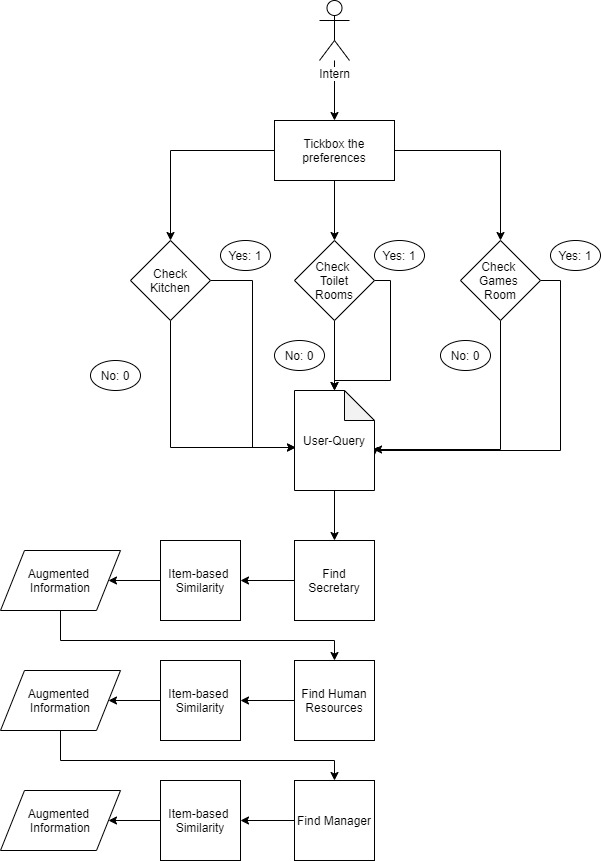
\includegraphics[scale=0.4]{Images/Chapter4/InternQuery.jpg}
    \caption[Inter User-Query Model]{Intern User-Query Model}
    \label{fig:InternQueryModel}
\end{figure}
\begin{figure}[H]
    \centering
    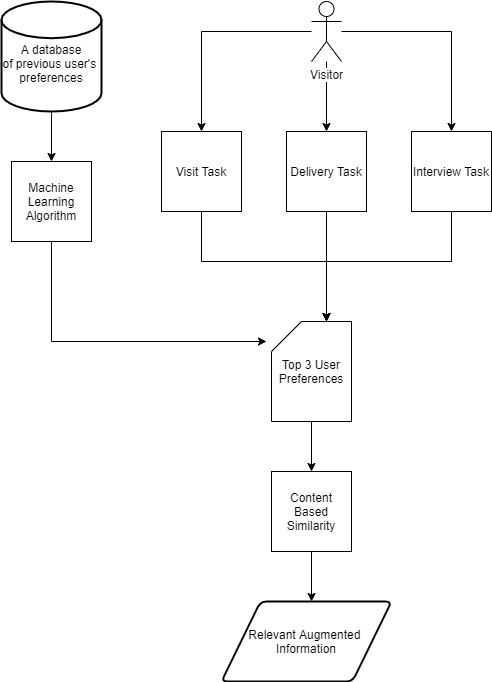
\includegraphics[scale=0.4]{Images/Chapter4/VisitorQueryModel.jpg}
    \captionof{figure}{Visitor User-Query Model}
    \label{fig:VisitorQueryModel}
\end{figure}
\begin{figure}[H]
    \centering
    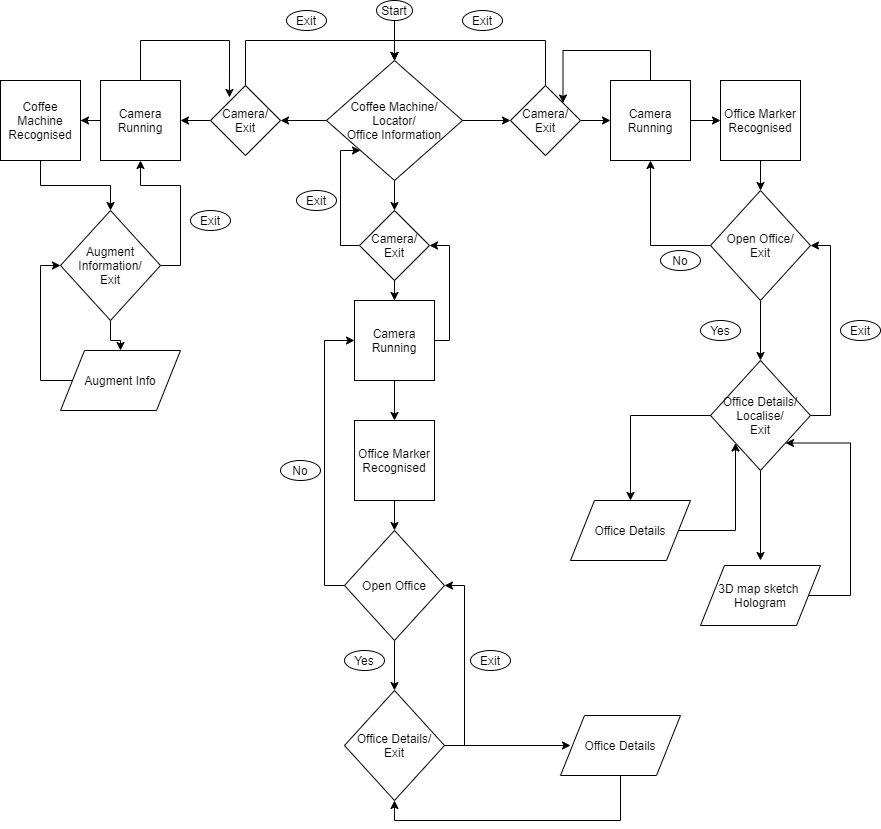
\includegraphics[scale=0.4]{Images/Chapter4/SystemArchitecture.jpg}
    \captionof{figure}{User-Interface and System Architecture}
    \label{fig:SystemArchitectureDesign}
\end{figure}
% ///////////////////////////////////////////////////////////////////////////////////////////////////
\section{Selecting AR markers}
    \begin{figure}[H]
    \centering
        \begin{minipage}{.5\textwidth}
          \centering
          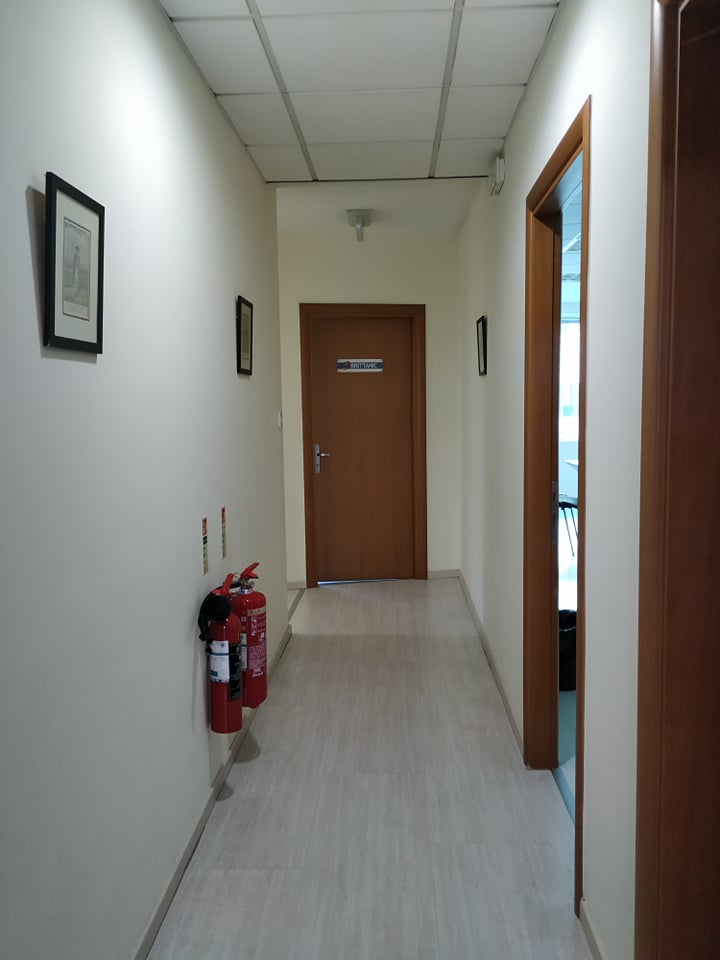
\includegraphics[scale=0.2]{Images/Chapter5/DatahandlingCorr.jpg}
          \captionof{figure}{Corridor Image Variation 1}
          \label{fig:test1}
        \end{minipage}%
        \begin{minipage}{.5\textwidth}
          \centering
          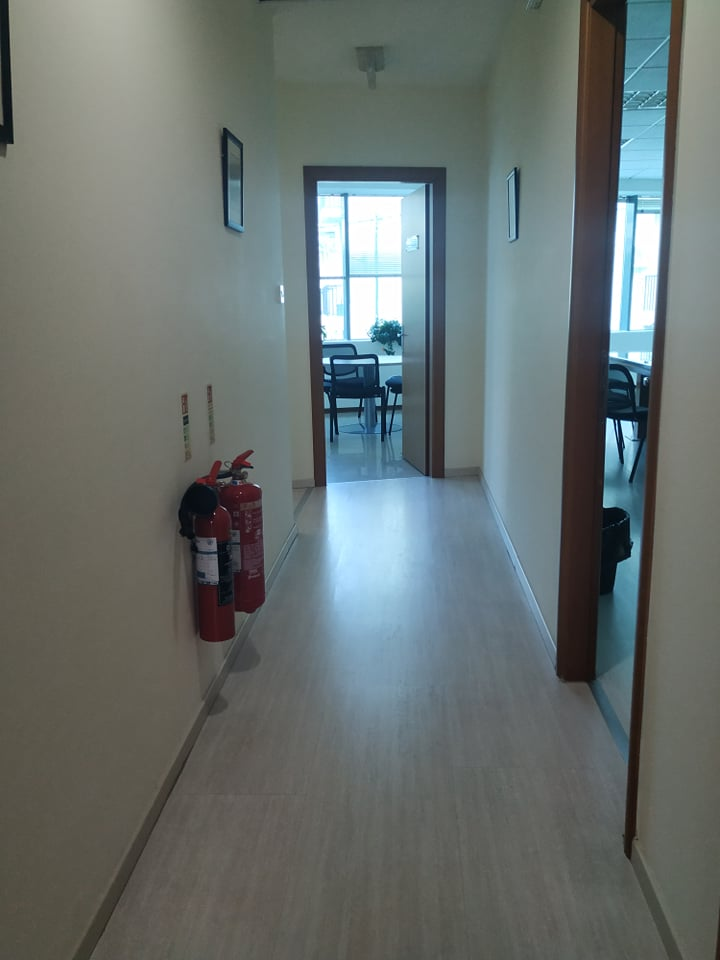
\includegraphics[scale=0.2]{Images/Chapter5/DatahandlingCorr2.jpg}
          \captionof{figure}{Corridor Image Variation 2}
          \label{fig:test2}
        \end{minipage}
    \end{figure}
    \begin{figure}[H]
    \centering
        \begin{minipage}{.5\textwidth}
          \centering
          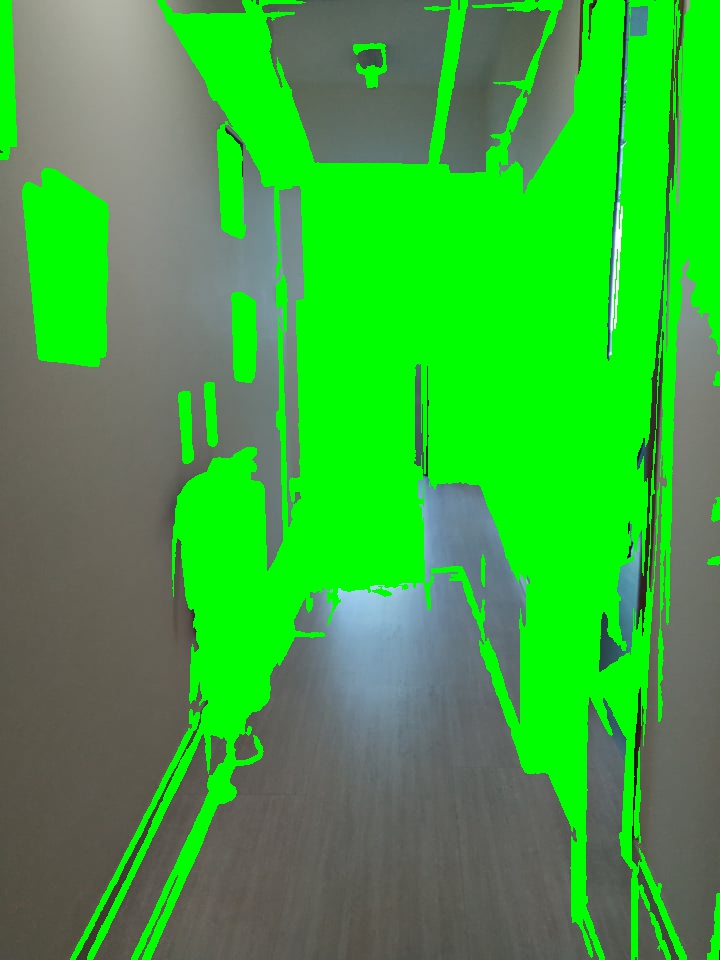
\includegraphics[scale=0.2]{Images/Chapter5/filled.jpg}
          \captionof{figure}{Result of differences using SSIM}
          \label{fig:test3}
        \end{minipage}%
        \begin{minipage}{.5\textwidth}
          \centering
          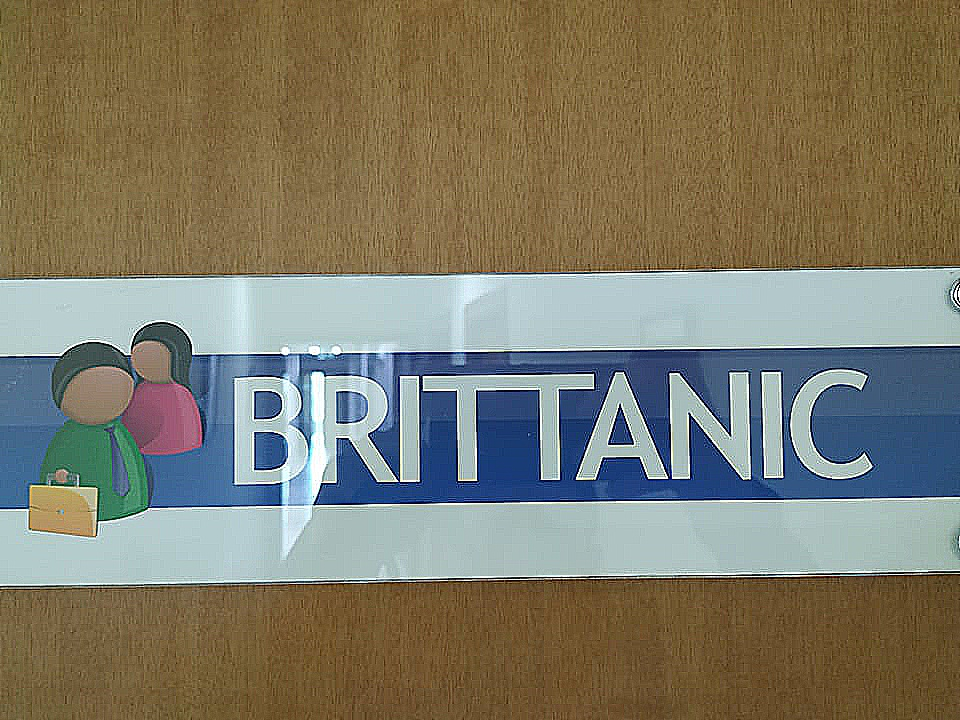
\includegraphics[scale=0.2]{Images/Chapter5/brittanicImproved.jpg}
          \captionof{figure}{Door Marker}
          \label{fig:test4}
        \end{minipage}
    \end{figure}
\section{Image and Model Targets}
    \begin{figure}[H]
    \centering
        \begin{minipage}{.5\textwidth}
          \centering
          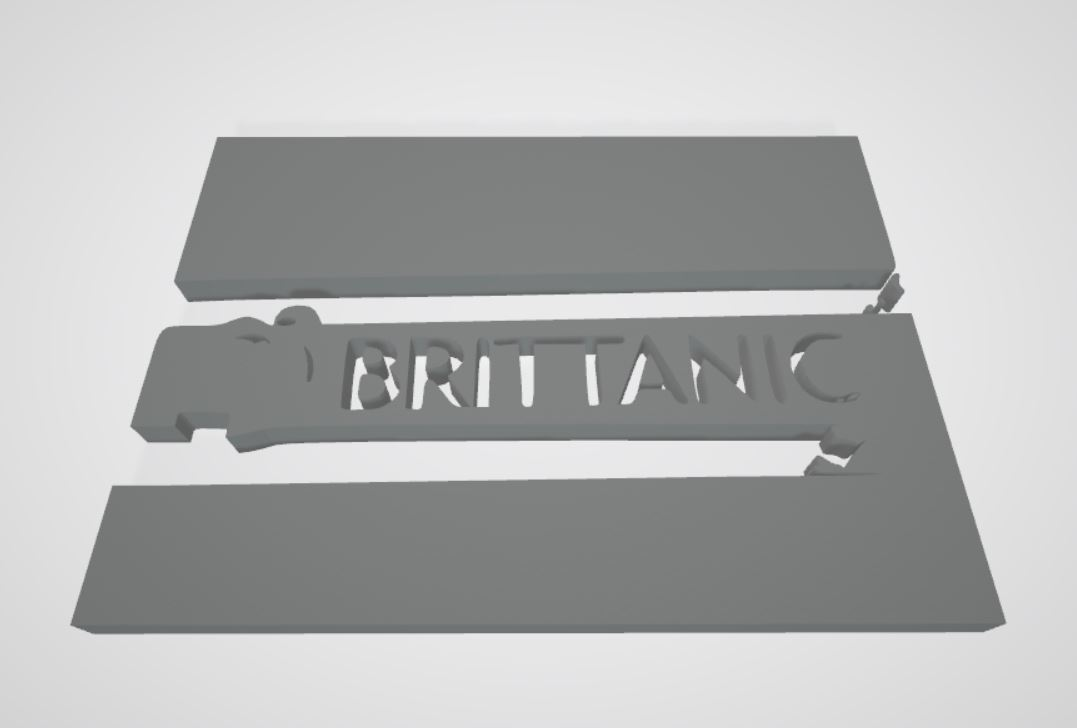
\includegraphics[scale=0.3]{Images/Chapter5/3DObject.JPG}
          \captionof{figure}{Door Marker 3D Object}
          \label{fig:test5}
        \end{minipage}%
        \begin{minipage}{.5\textwidth}
          \centering
          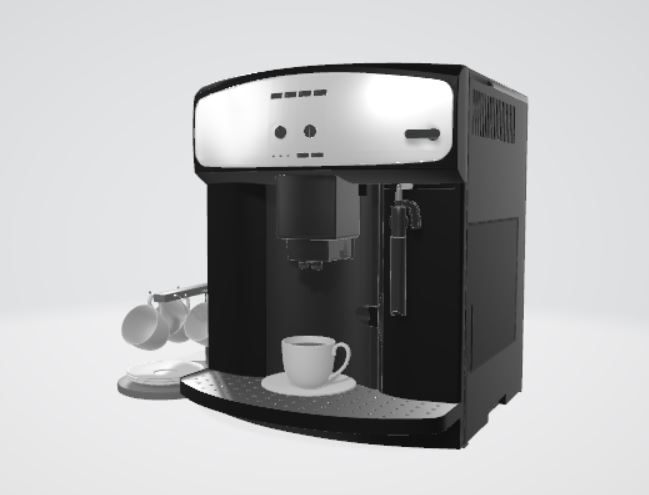
\includegraphics[scale=0.3]{Images/Chapter5/CoffeeMachine3DObject.JPG}
          \captionof{figure}{Coffee Machine 3D Object}
          \label{fig:test6}
        \end{minipage}
    \end{figure}
    \begin{figure}[H]
    \centering
        \begin{minipage}{.5\textwidth}
          \centering
          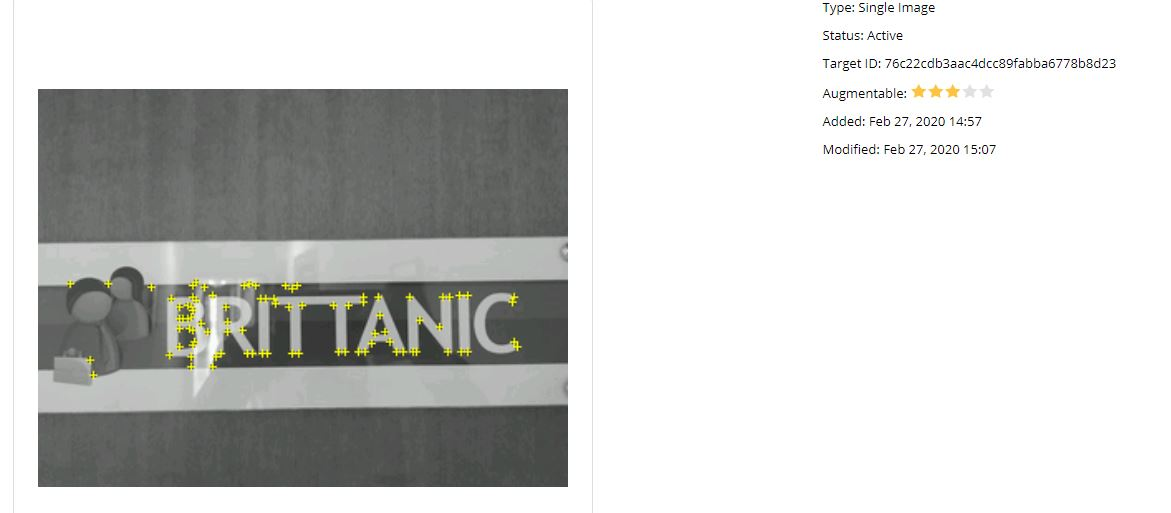
\includegraphics[scale=0.5]{Images/Chapter5/ImageTarget.JPG}
          \captionof{figure}{Image Target}
          \label{fig:test7}
        \end{minipage}%
    \end{figure}
    \begin{figure}[H]
    \centering
          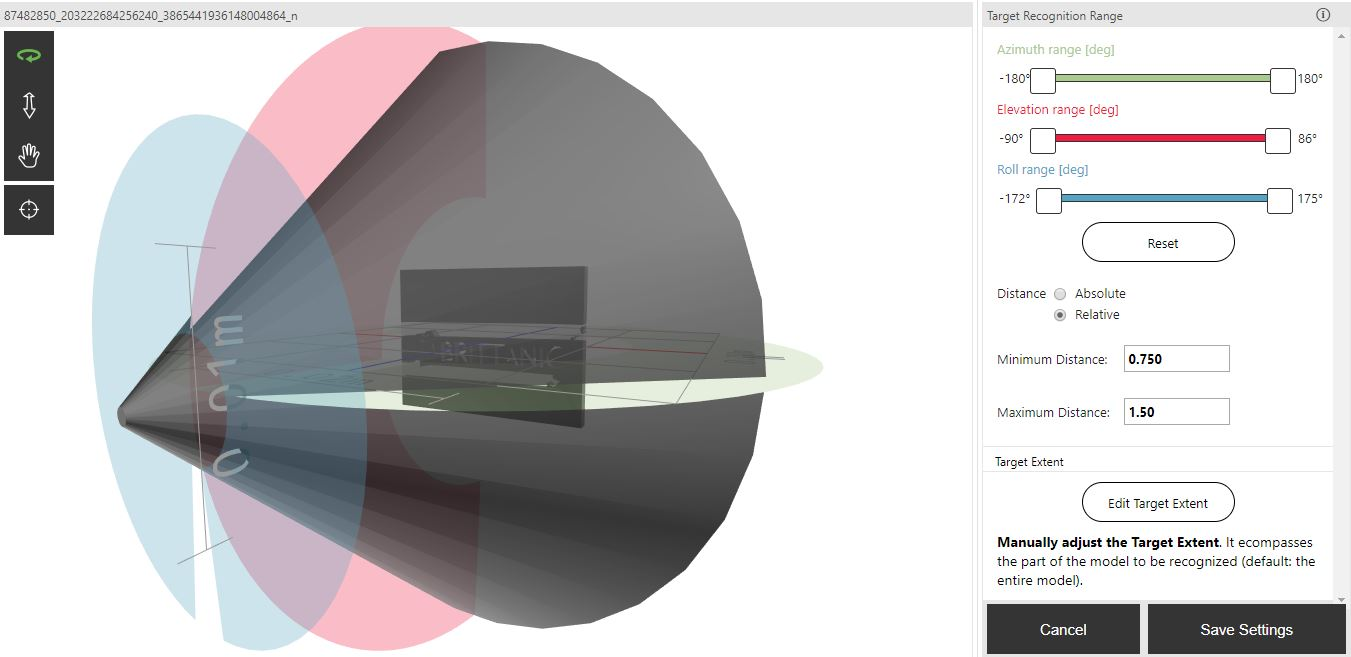
\includegraphics[scale=0.4]{Images/Chapter5/ModelTarget.JPG}
          \captionof{figure}{Model Target}
          \label{fig:test8}
    \end{figure}
\newpage
\section{Vuforia AR SDK}
\begin{figure}[H]
    \centering

          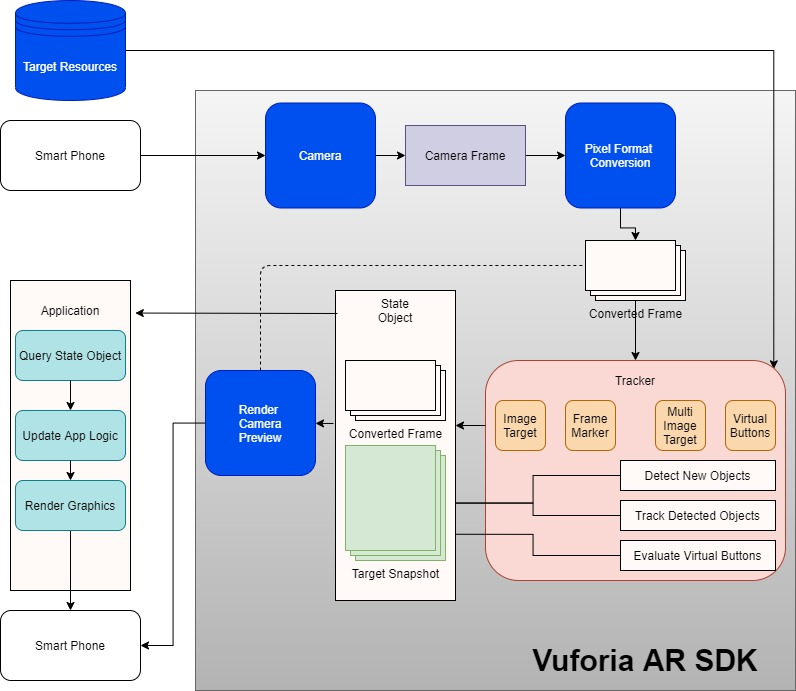
\includegraphics[scale=0.4]{Images/Chapter5/VuforiaARSDK.jpg}
          \captionof{figure}{Vuforia AR SDK as found in \cite{Ibez2013VuforiaVS}}
          \label{fig:VuforiaARSDK}
\end{figure}
\section{Implementation Examples}
\begin{figure}[H]
    \centering
        \begin{minipage}{.5\textwidth}
          \centering
          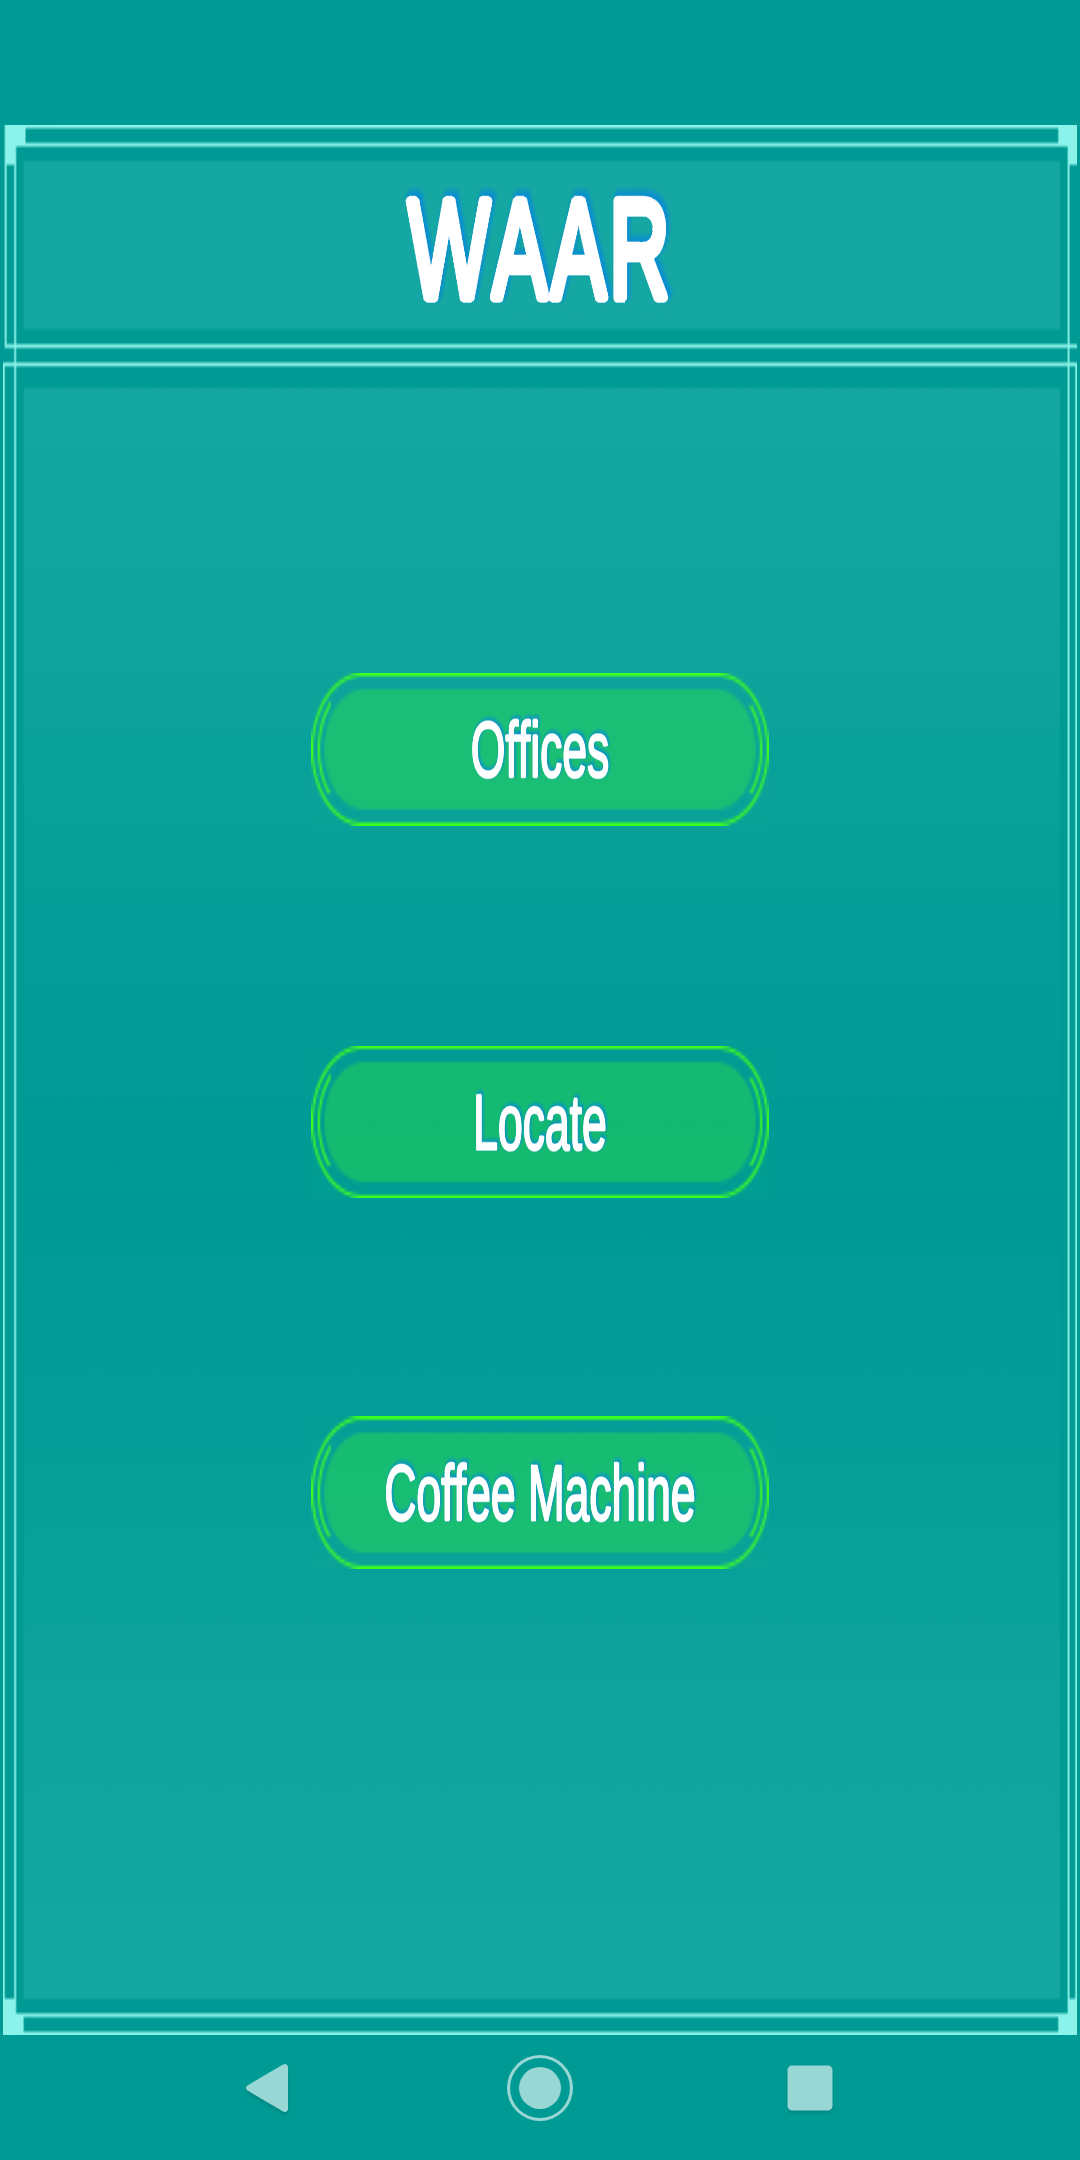
\includegraphics[scale=0.2]{Images/Chapter5/Impl3.png}
          \captionof{figure}{Main Menu}
          \label{fig:MainMenu}
        \end{minipage}%
        \begin{minipage}{.5\textwidth}
          \centering
          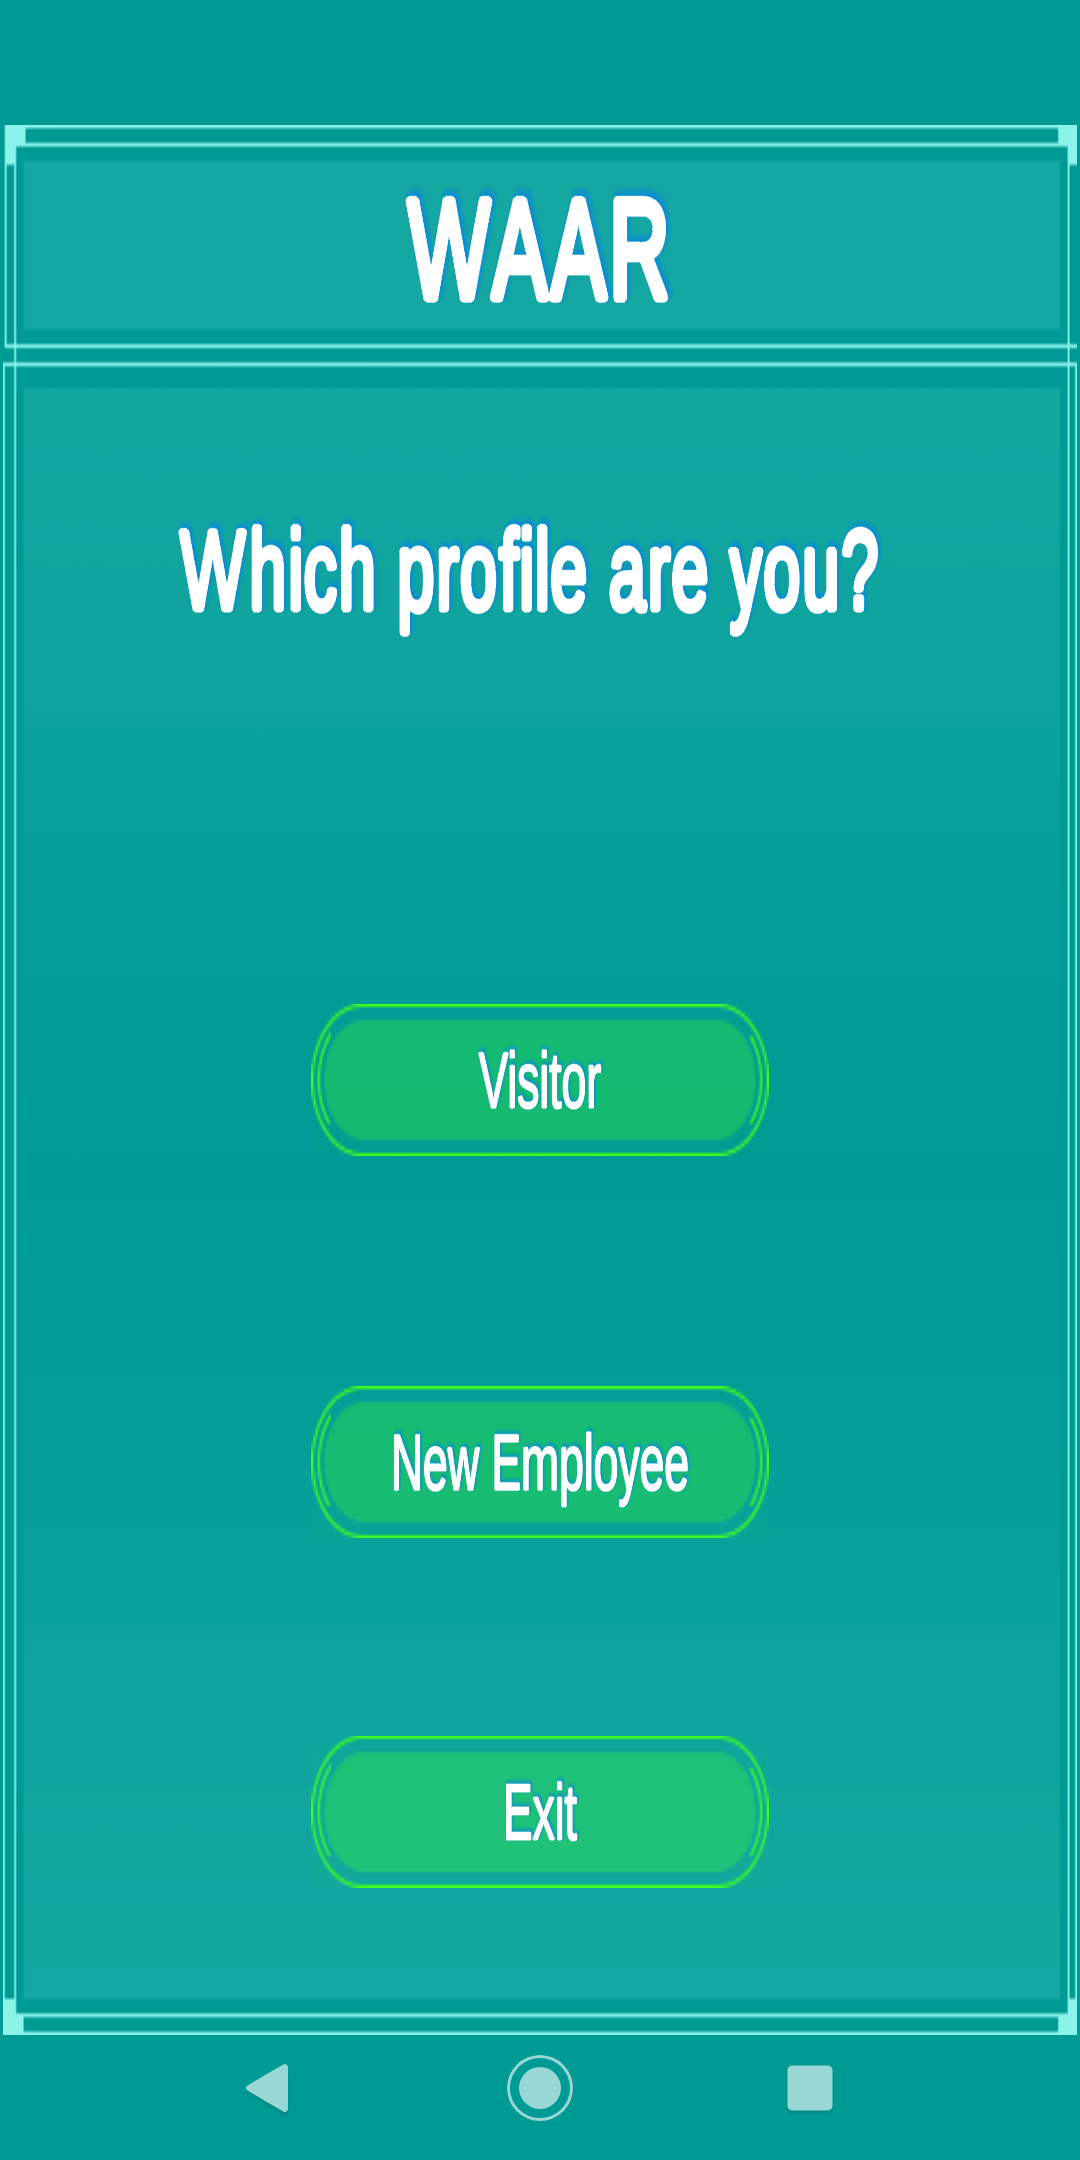
\includegraphics[scale=0.2]{Images/Chapter5/Impl2.png}
          \captionof{figure}{Choosing user profile}
          \label{fig:UserProfile}
        \end{minipage}
\end{figure}
\begin{figure}[H]
    \centering
        \begin{minipage}{.5\textwidth}
          \centering
          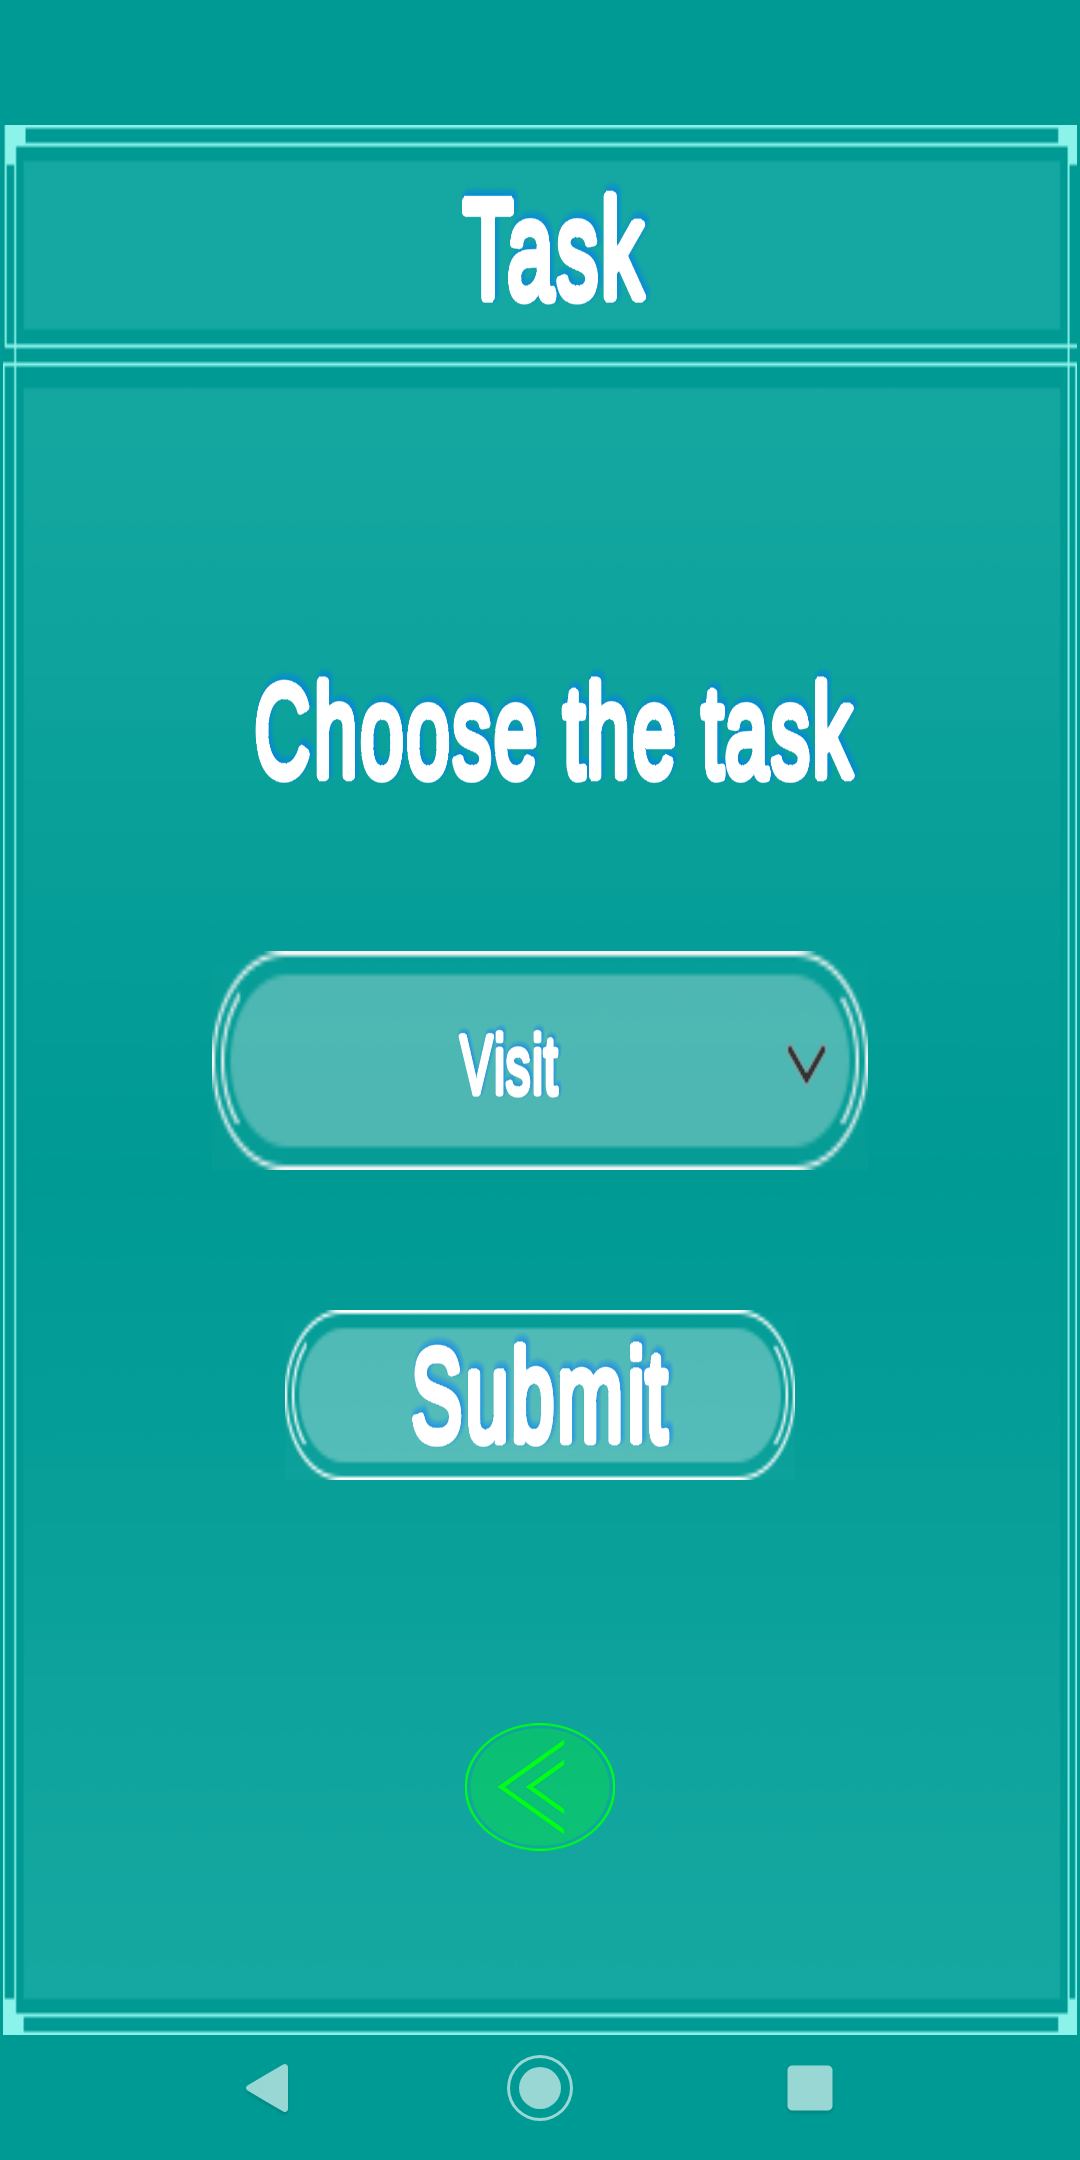
\includegraphics[scale=0.2]{Images/Chapter5/Impl13.png}
          \captionof{figure}{Choosing a visitor task}
          \label{fig:TaskMenu}
        \end{minipage}%
        \begin{minipage}{.5\textwidth}
          \centering
          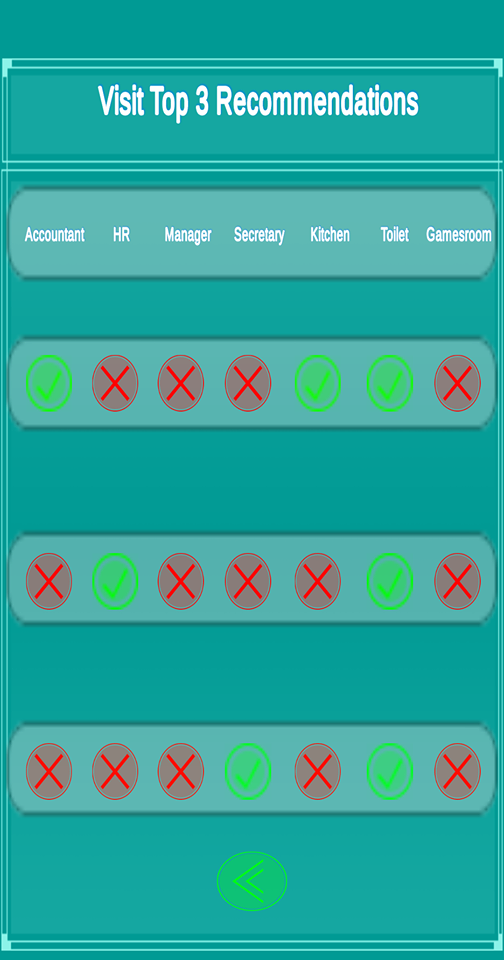
\includegraphics[scale=0.45]{Images/Chapter5/Impl1.png}
          \captionof{figure}{Visitor Recommendation for Visit}
          \label{fig:VisitRecommendations}
        \end{minipage}
\end{figure}
\begin{figure}[H]
    \centering
        \begin{minipage}{.5\textwidth}
          \centering
          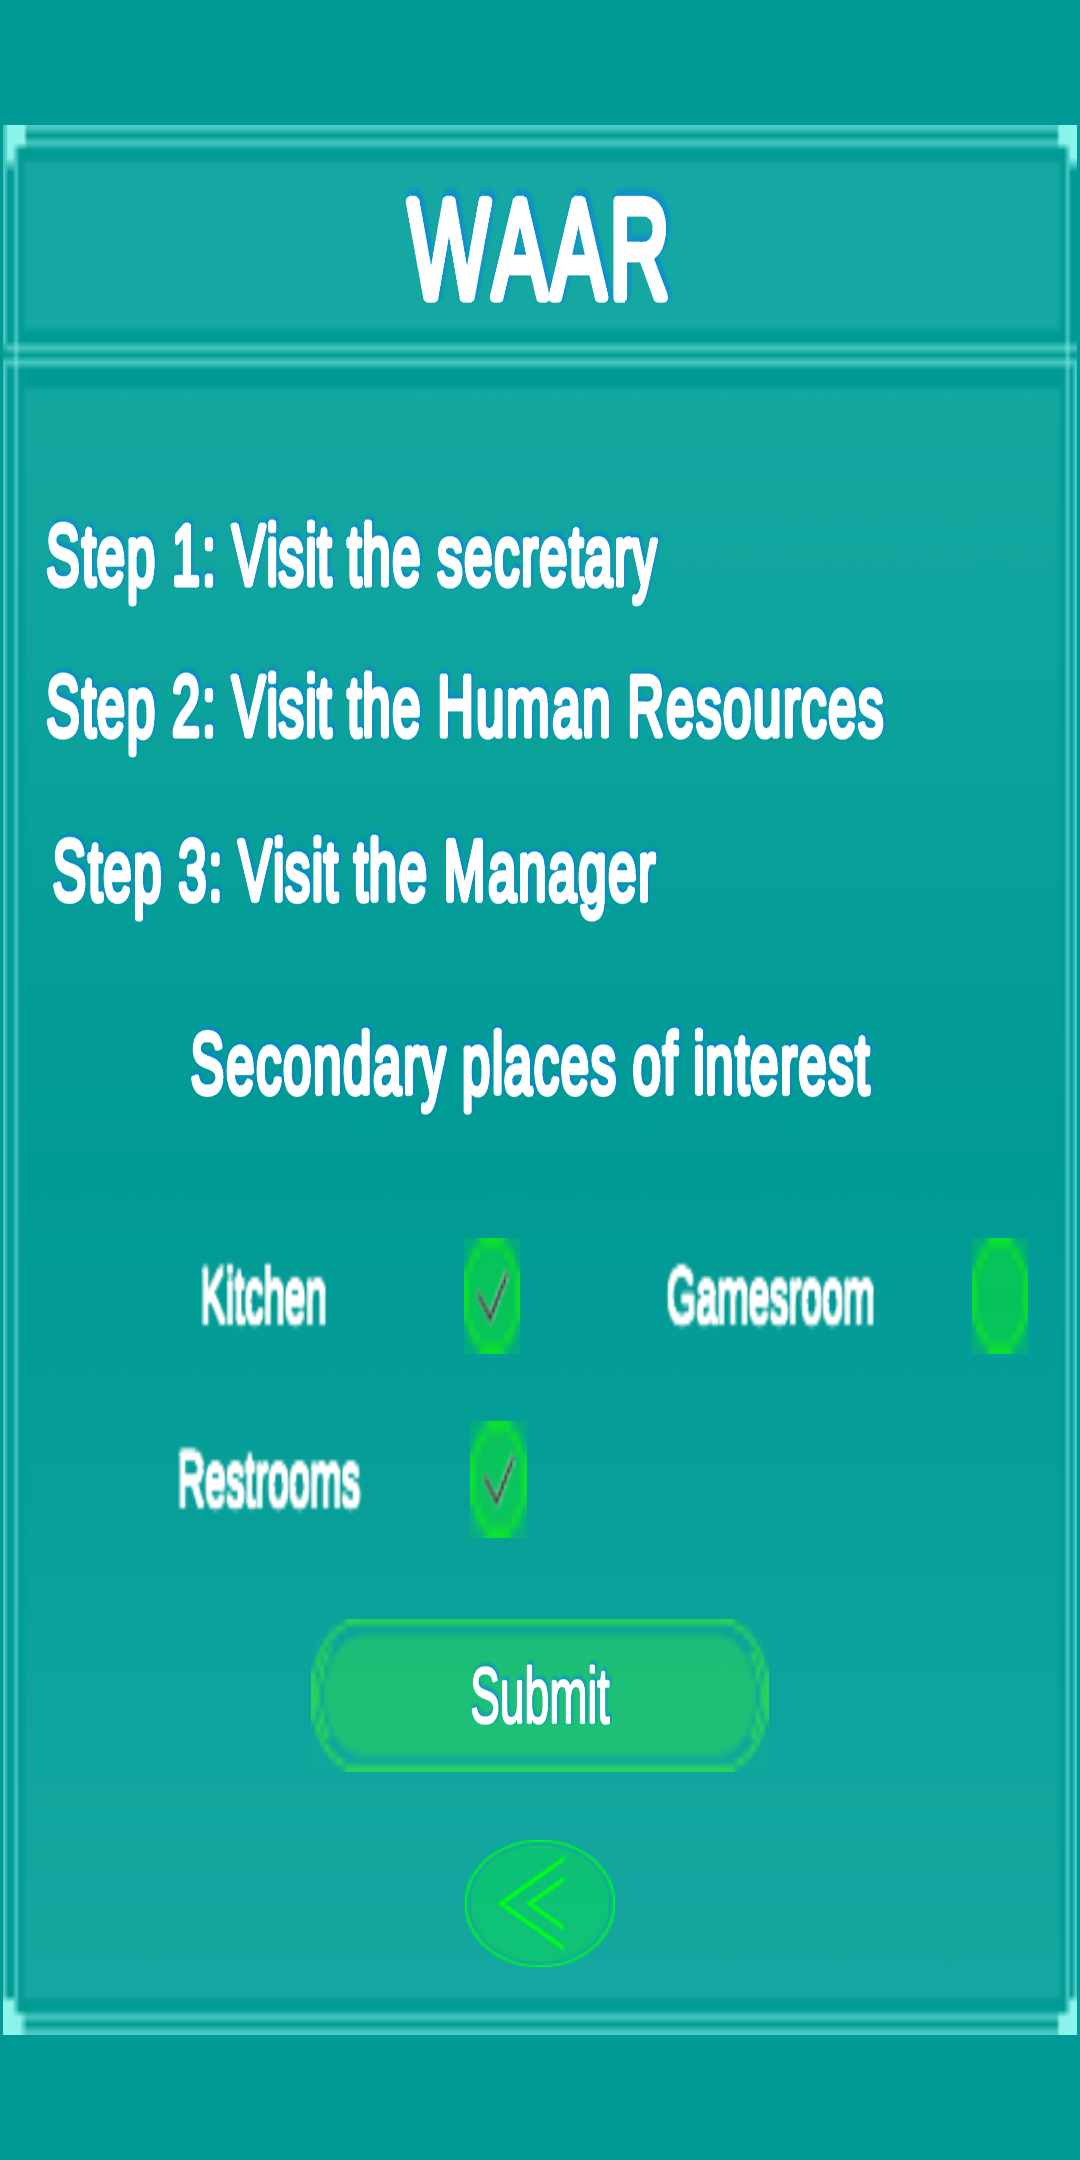
\includegraphics[scale=0.2]{Images/Chapter5/Impl12.png}
          \captionof{figure}{Intern Locations of interest menu}
          \label{fig:InternsMenu}
        \end{minipage}%
        \begin{minipage}{.5\textwidth}
          \centering
          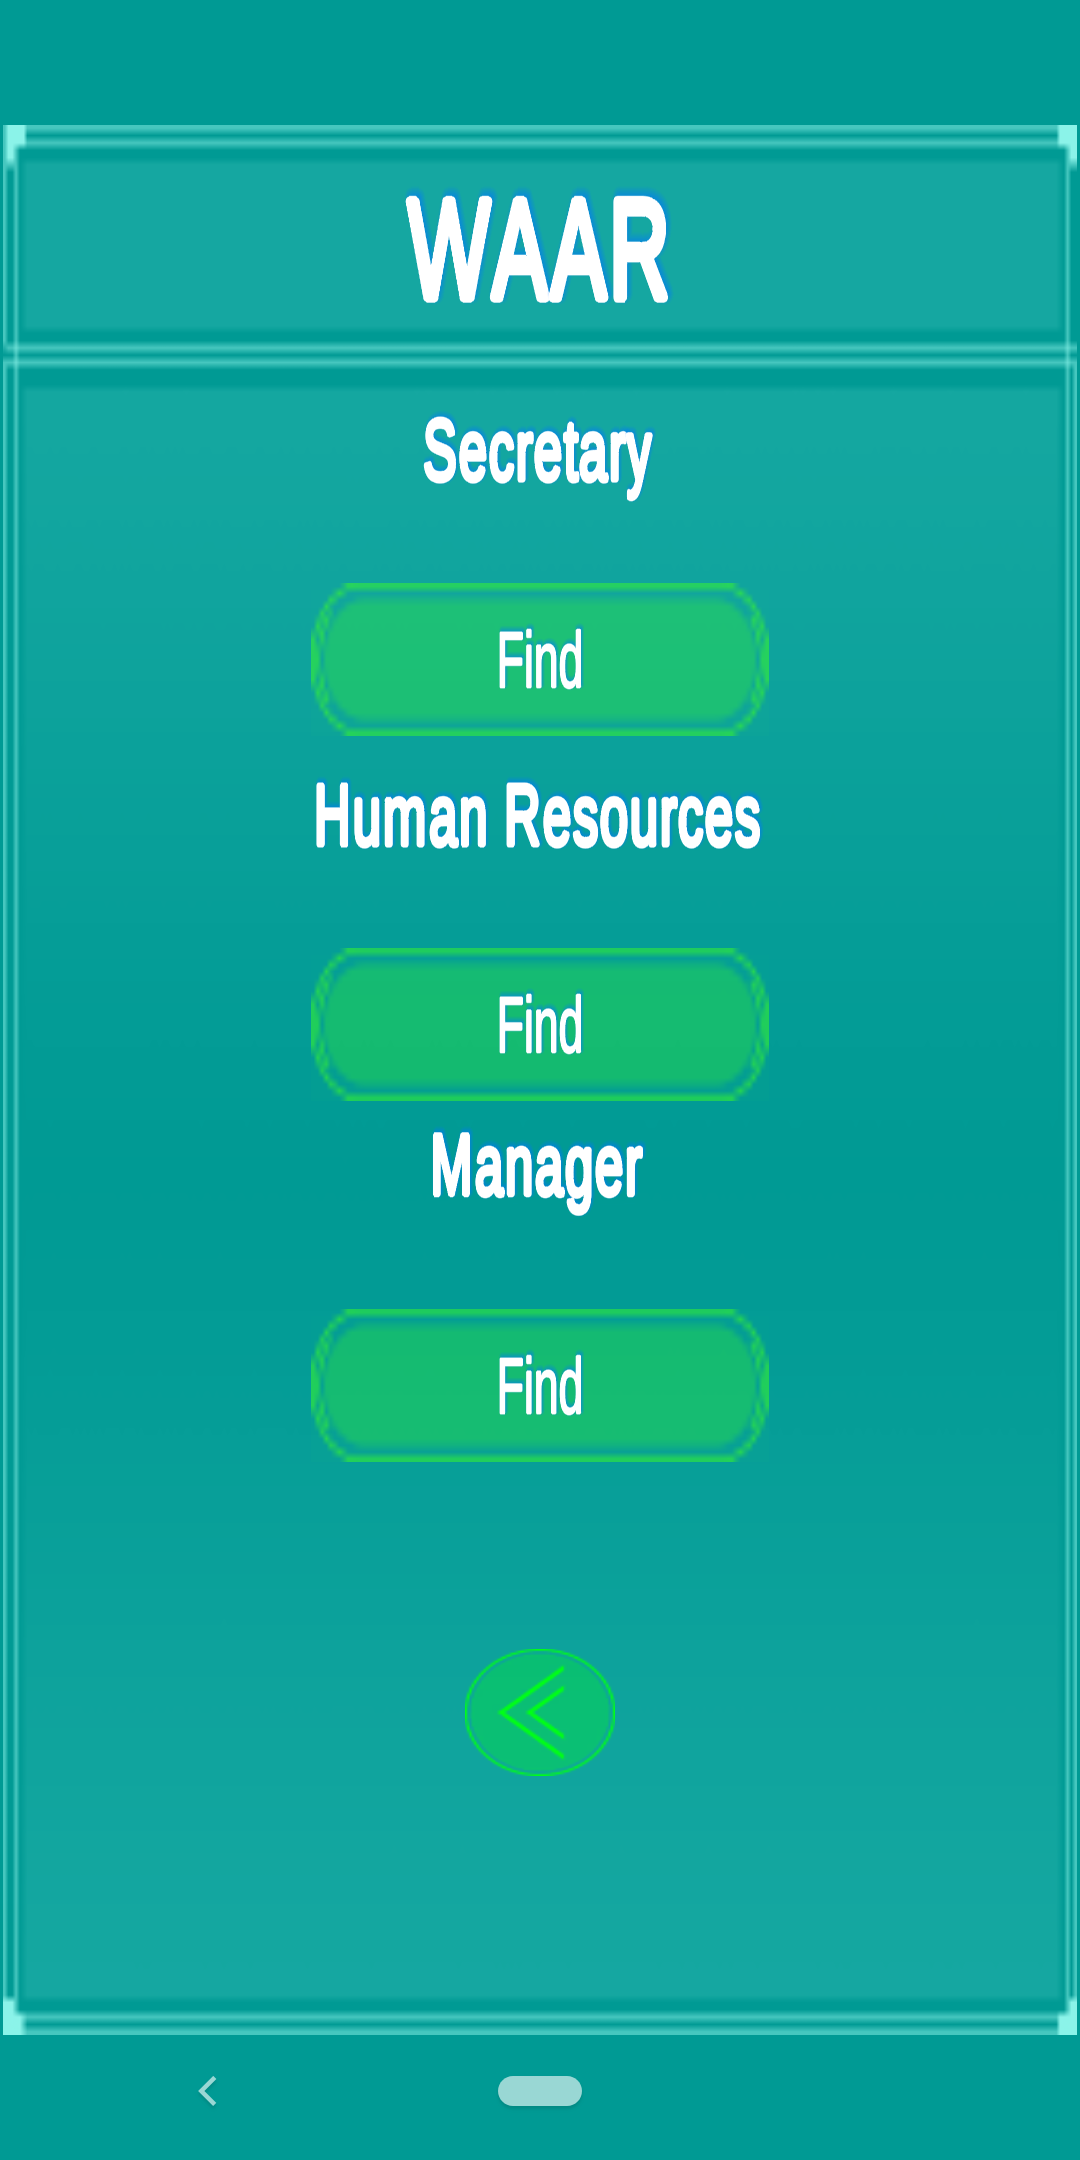
\includegraphics[scale=0.2]{Images/Chapter5/Impl19.png}
          \captionof{figure}{Intern's first day of adjustments}
          \label{fig:InternsProcedure}
        \end{minipage}
\end{figure}
\begin{figure}[H]
    \centering
        \begin{minipage}{.5\textwidth}
          \centering
          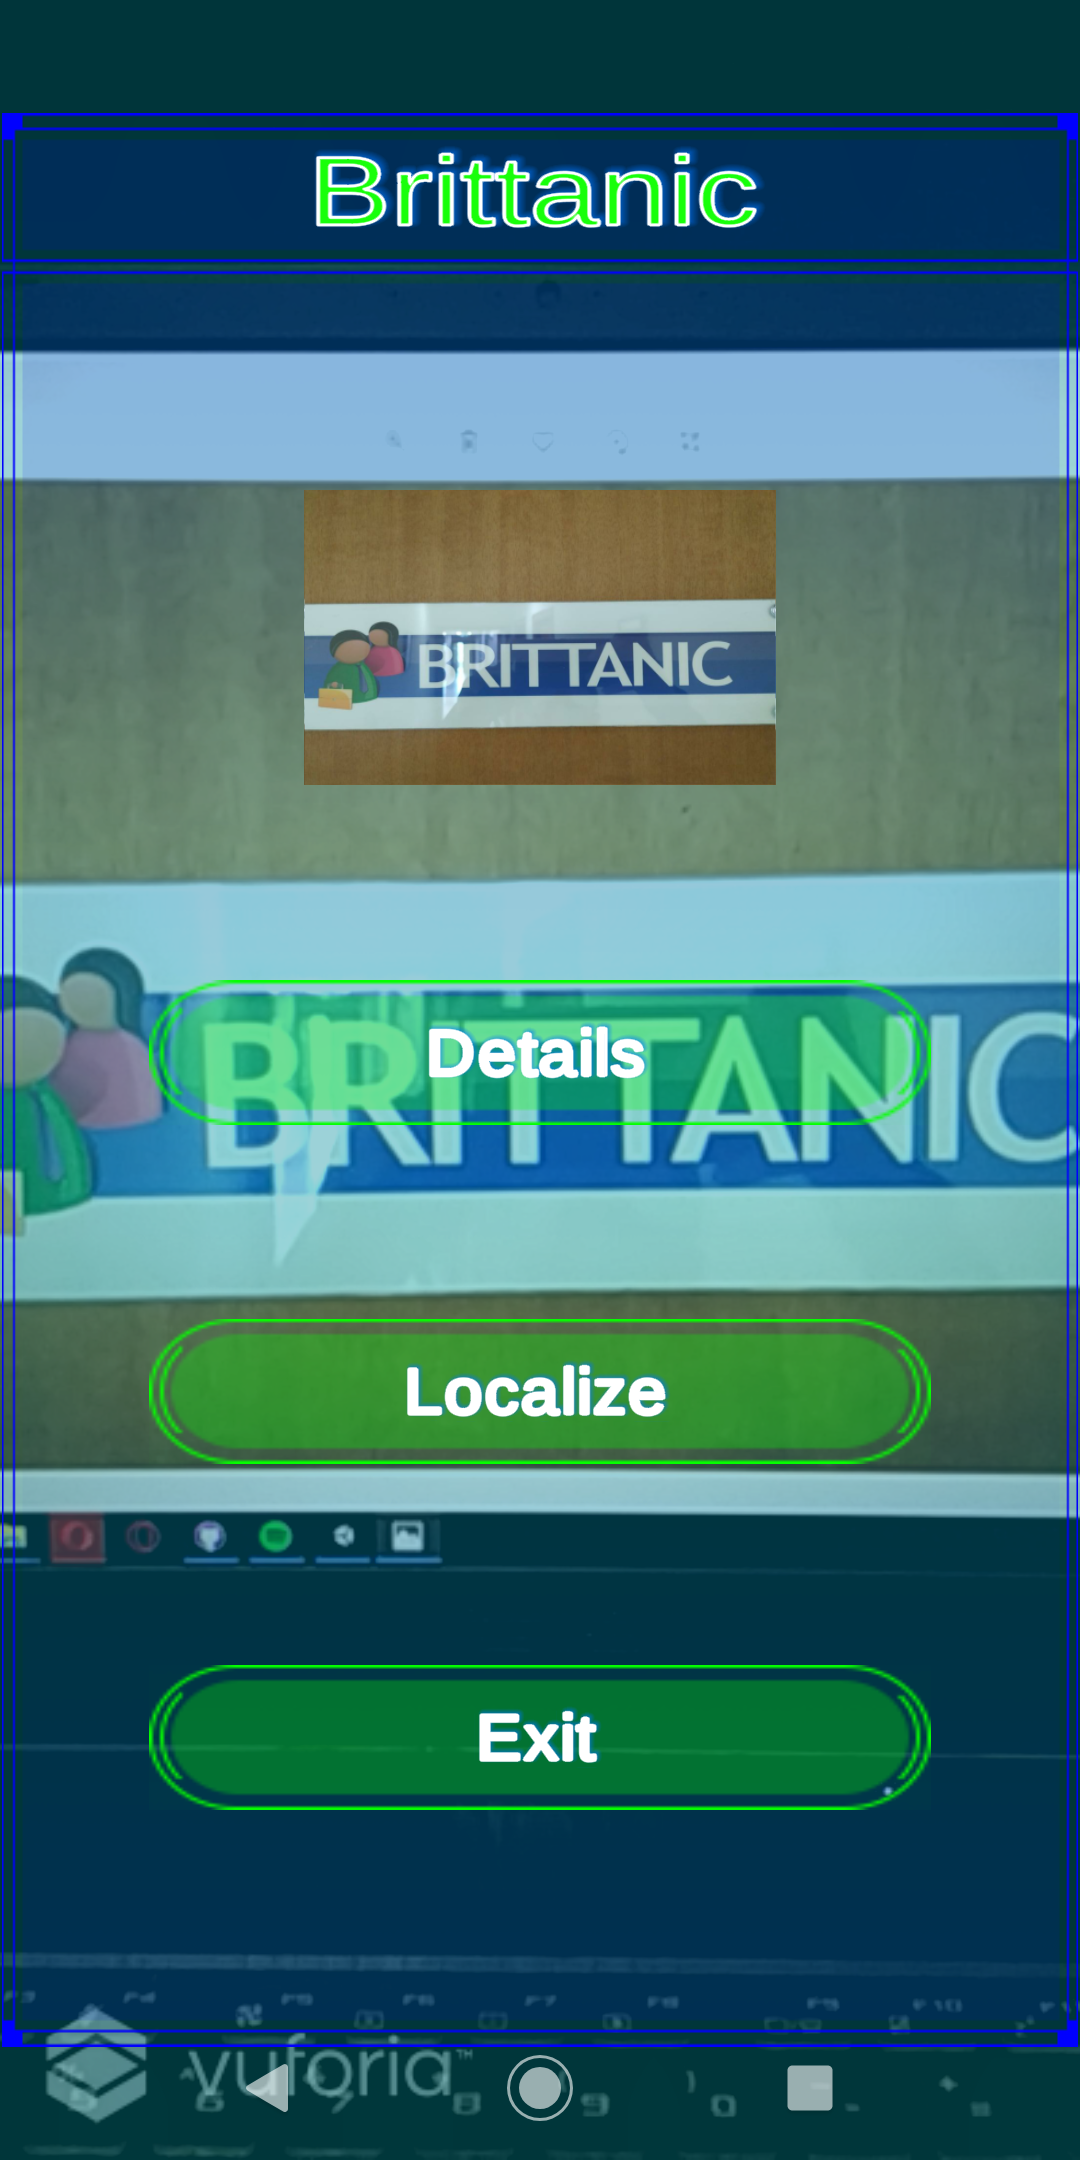
\includegraphics[scale=0.2]{Images/Chapter5/Impl11.png}
          \captionof{figure}{Marker Augmentation Menu}
          \label{fig:AugmentationMenu}
        \end{minipage}%
        \begin{minipage}{.5\textwidth}
          \centering
          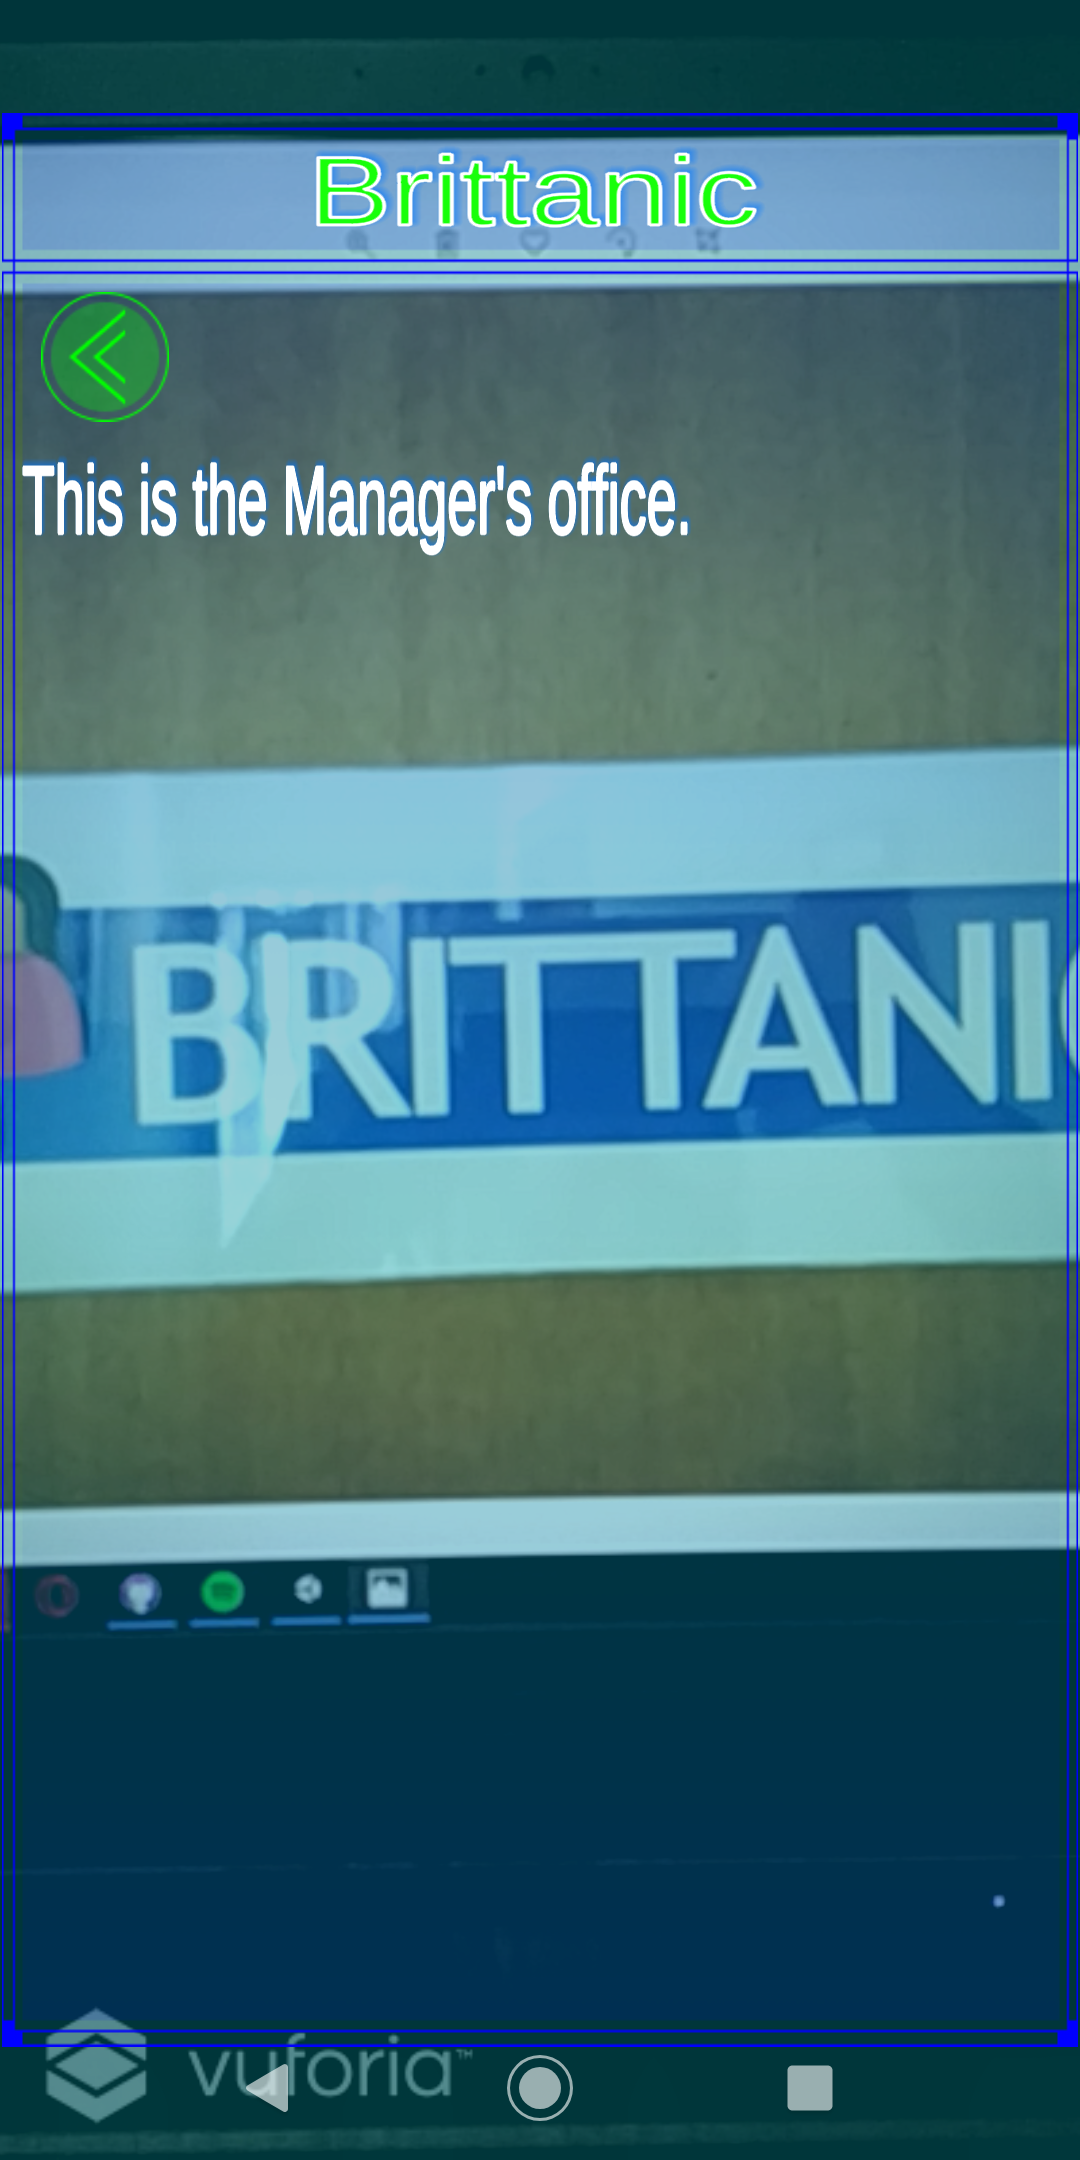
\includegraphics[scale=0.2]{Images/Chapter5/Impl8.png}
          \captionof{figure}{Office Details}
          \label{fig:Details}
        \end{minipage}
\end{figure}
\begin{figure}[H]
    \centering
        \begin{minipage}{.5\textwidth}
          \centering
          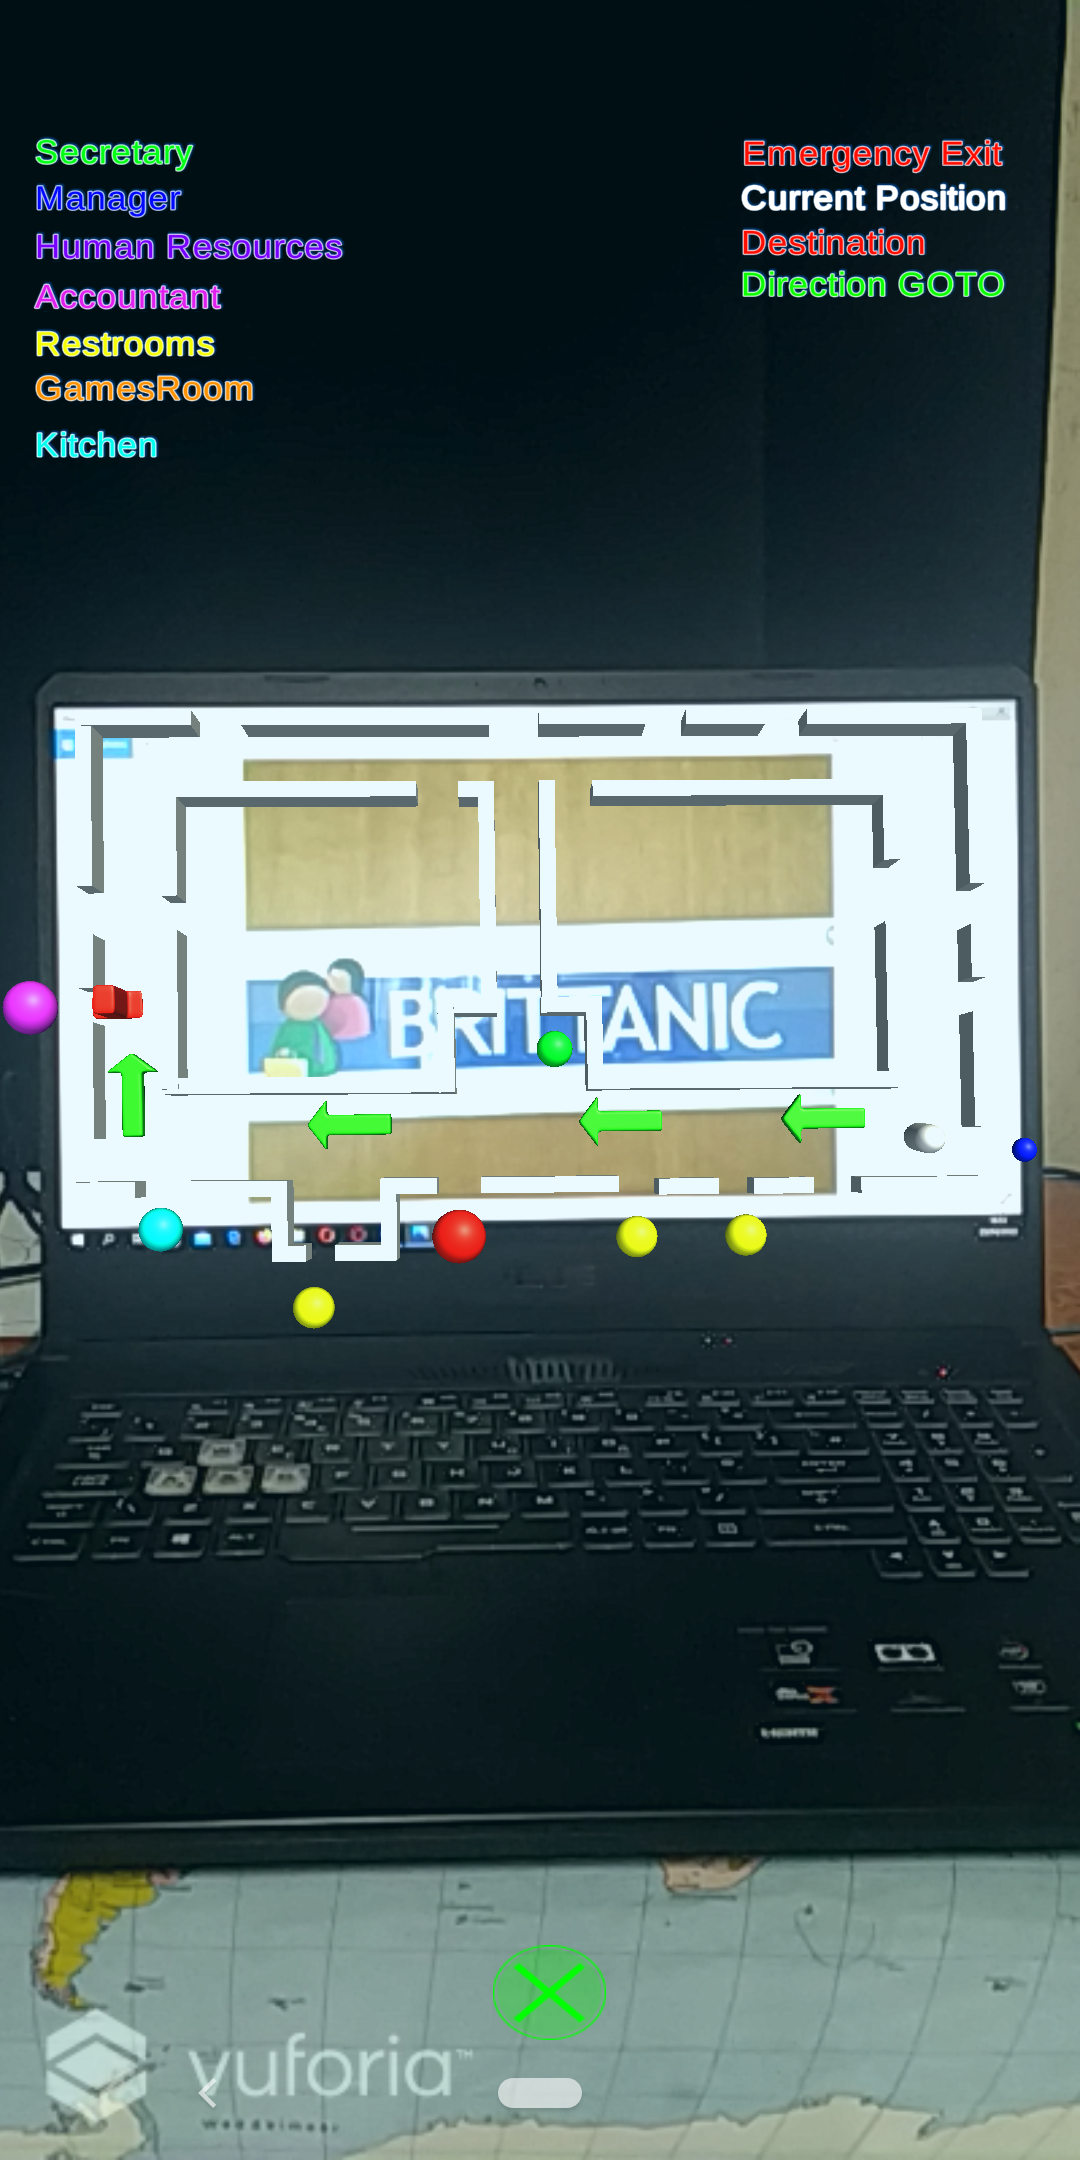
\includegraphics[scale=0.2]{Images/Chapter5/Impl10.png}
          \captionof{figure}{Holographic Sketch Map Front View}
          \label{fig:MapFrontView}
        \end{minipage}%
        \begin{minipage}{.5\textwidth}
          \centering
          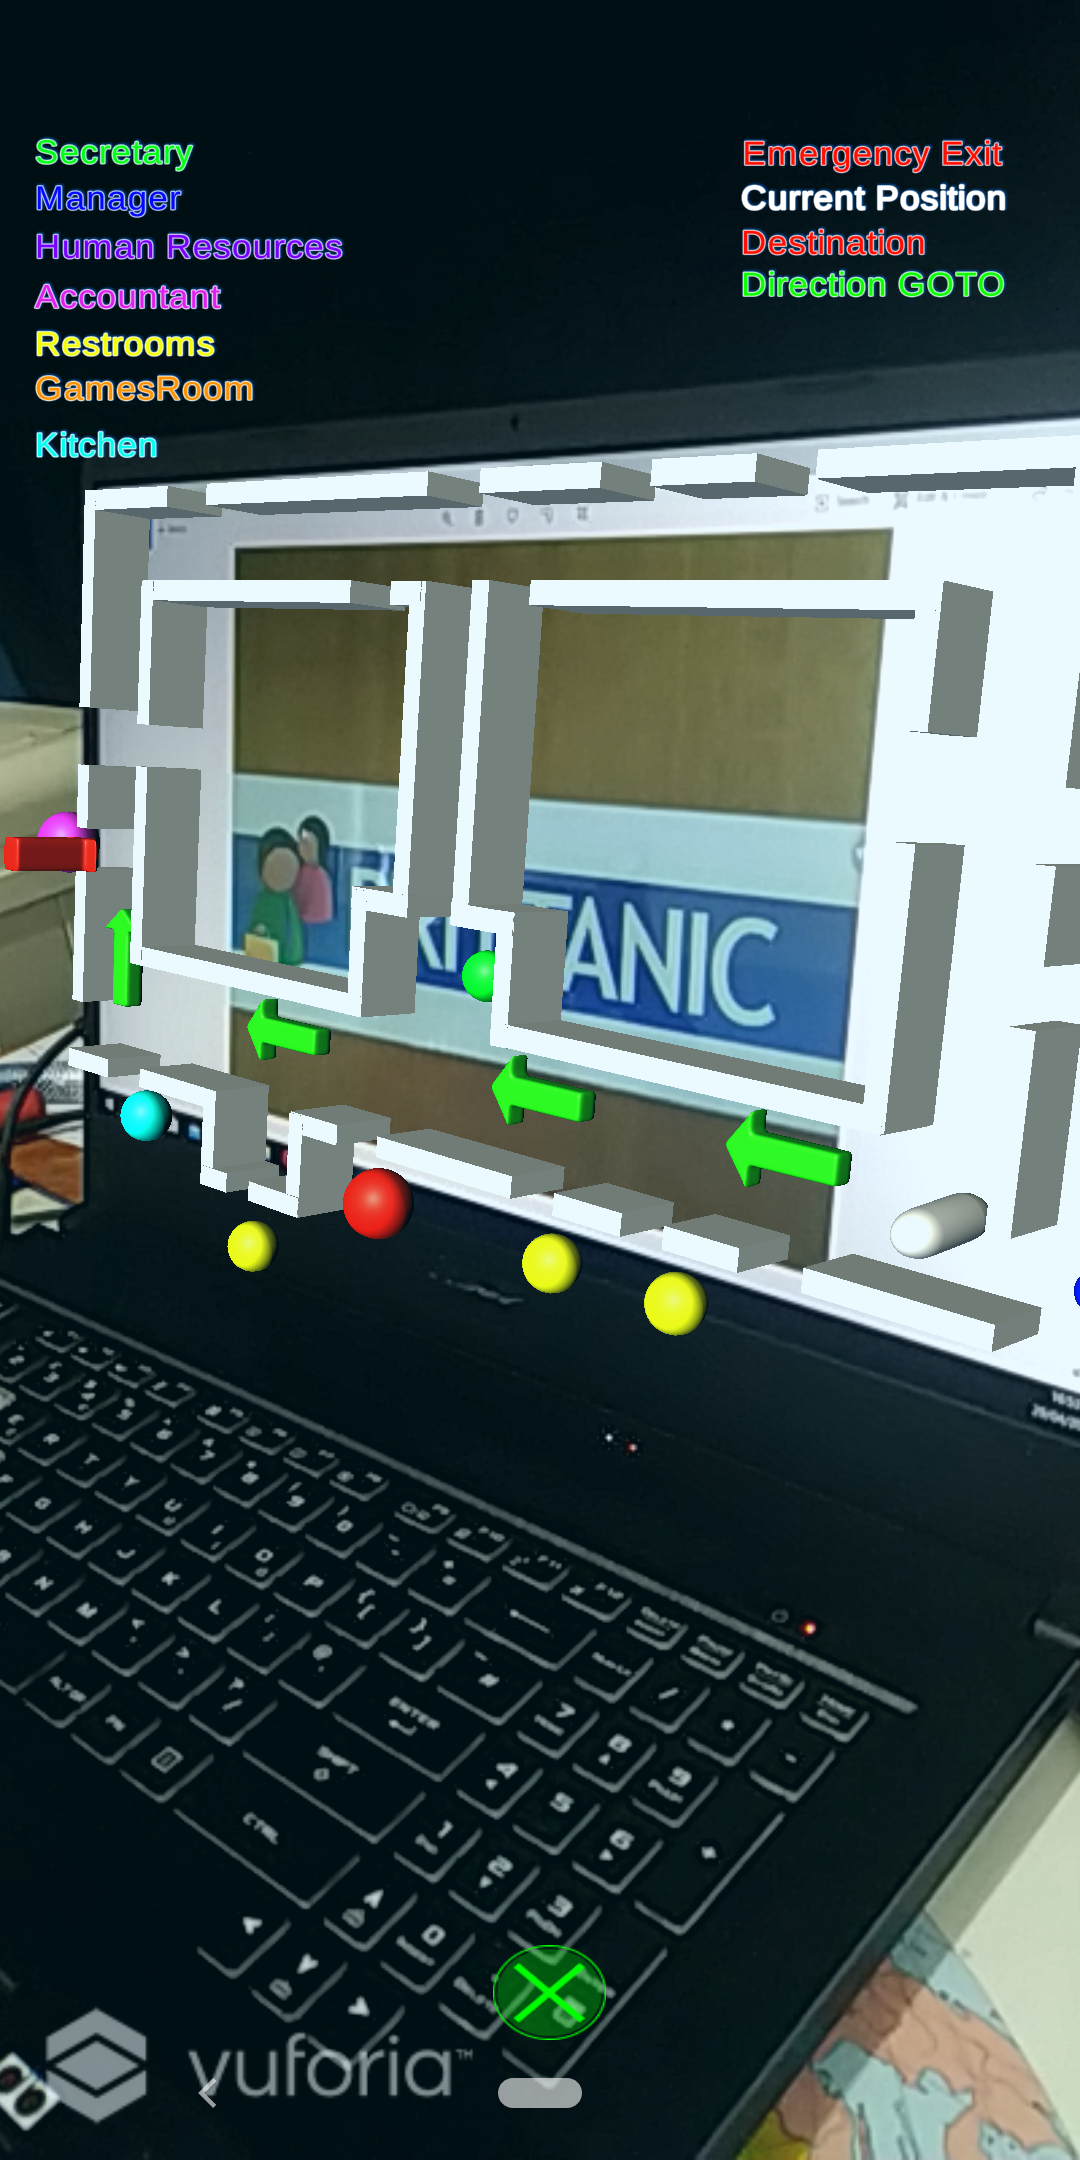
\includegraphics[scale=0.2]{Images/Chapter5/Impl9.png}
          \captionof{figure}{Holographic Sketch Map Side View}
          \label{fig:MapSideView}
        \end{minipage}
\end{figure}
\begin{figure}[H]
    \centering
        \begin{minipage}{.5\textwidth}
          \centering
          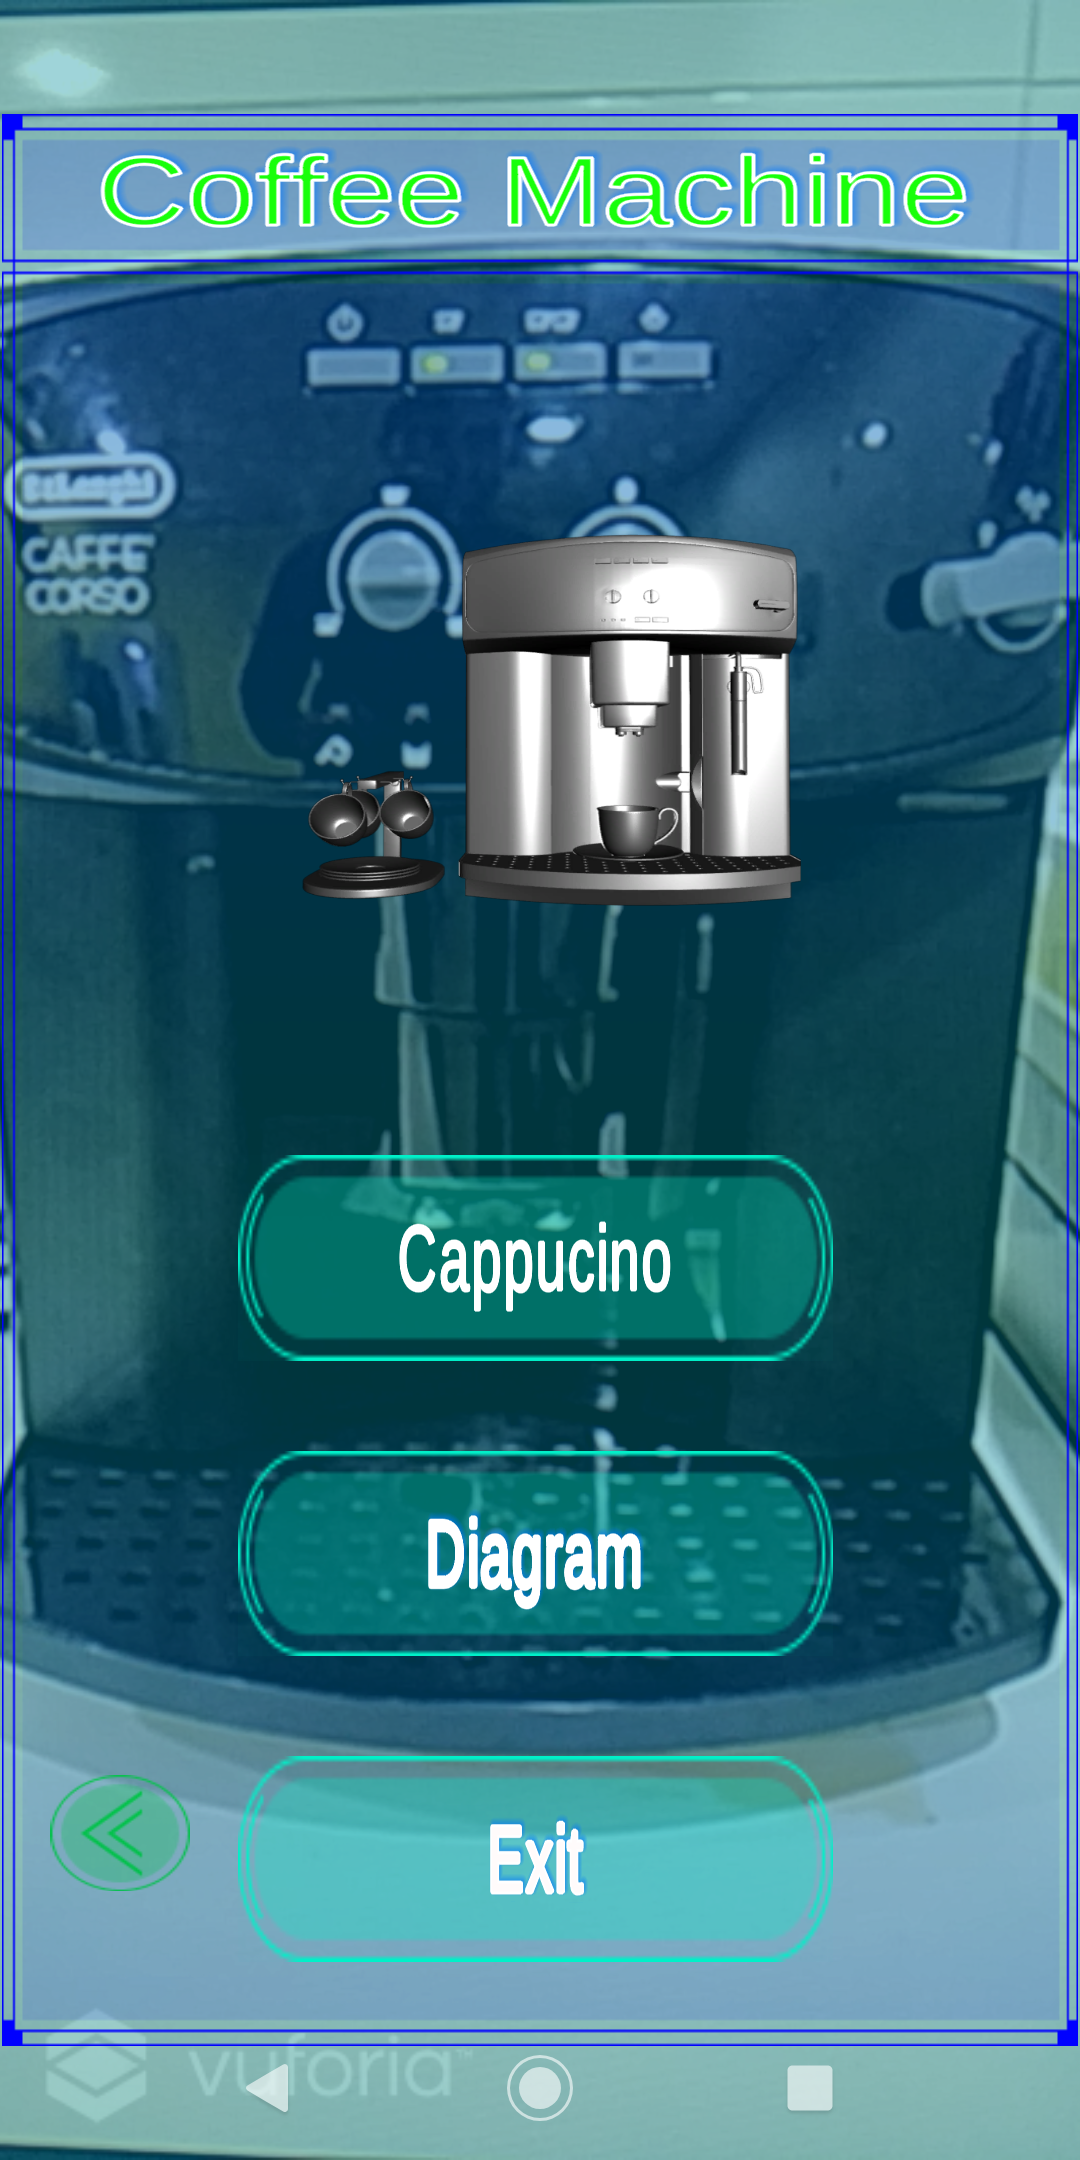
\includegraphics[scale=0.2]{Images/Chapter5/Impl7.png}
          \captionof{figure}{Coffee Machine Augmentation Menu}
          \label{fig:CoffeeMachineAugmentationMenu}
        \end{minipage}%
        \begin{minipage}{.5\textwidth}
          \centering
          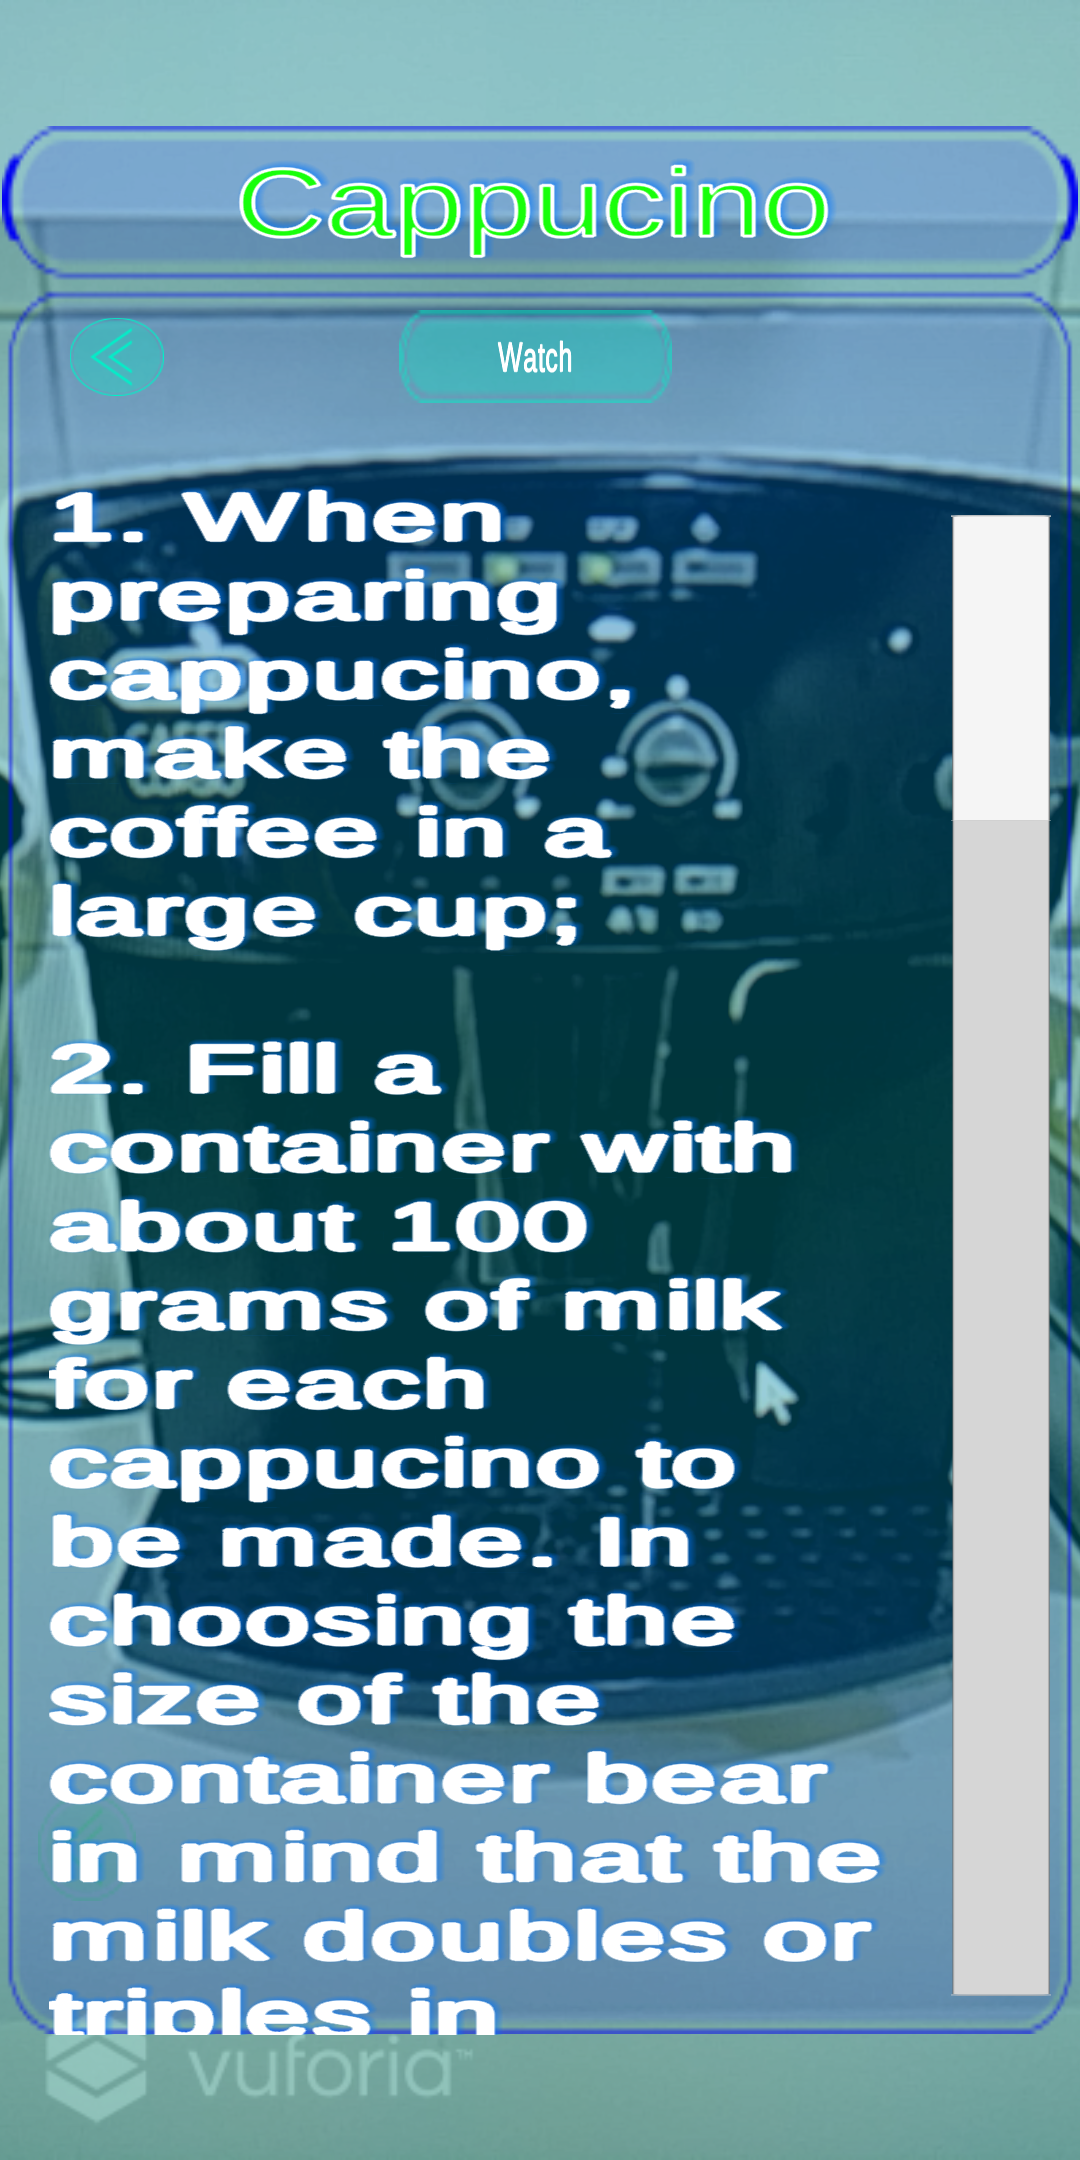
\includegraphics[scale=0.2]{Images/Chapter5/Impl16Overwritten.png}
          \captionof{figure}{Cappuccino Details}
          \label{fig:CappuccinoDetails}
        \end{minipage}
\end{figure}
\begin{figure}[H]
    \centering
        \begin{minipage}{.5\textwidth}
          \centering
          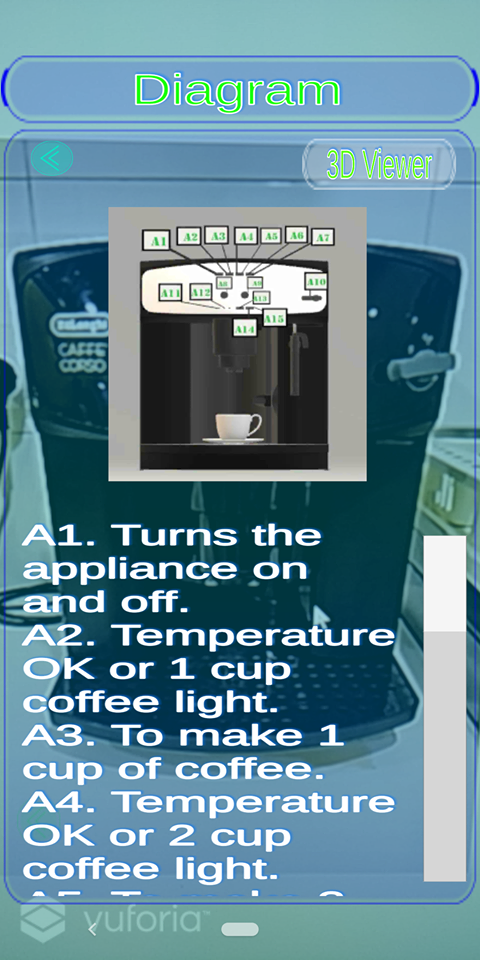
\includegraphics[scale=0.45]{Images/Chapter5/Impl5.png}
          \captionof{figure}{Coffee Machine Diagram}
          \label{fig:CoffeeMachineDiagram}
        \end{minipage}%
        \begin{minipage}{.5\textwidth}
          \centering
          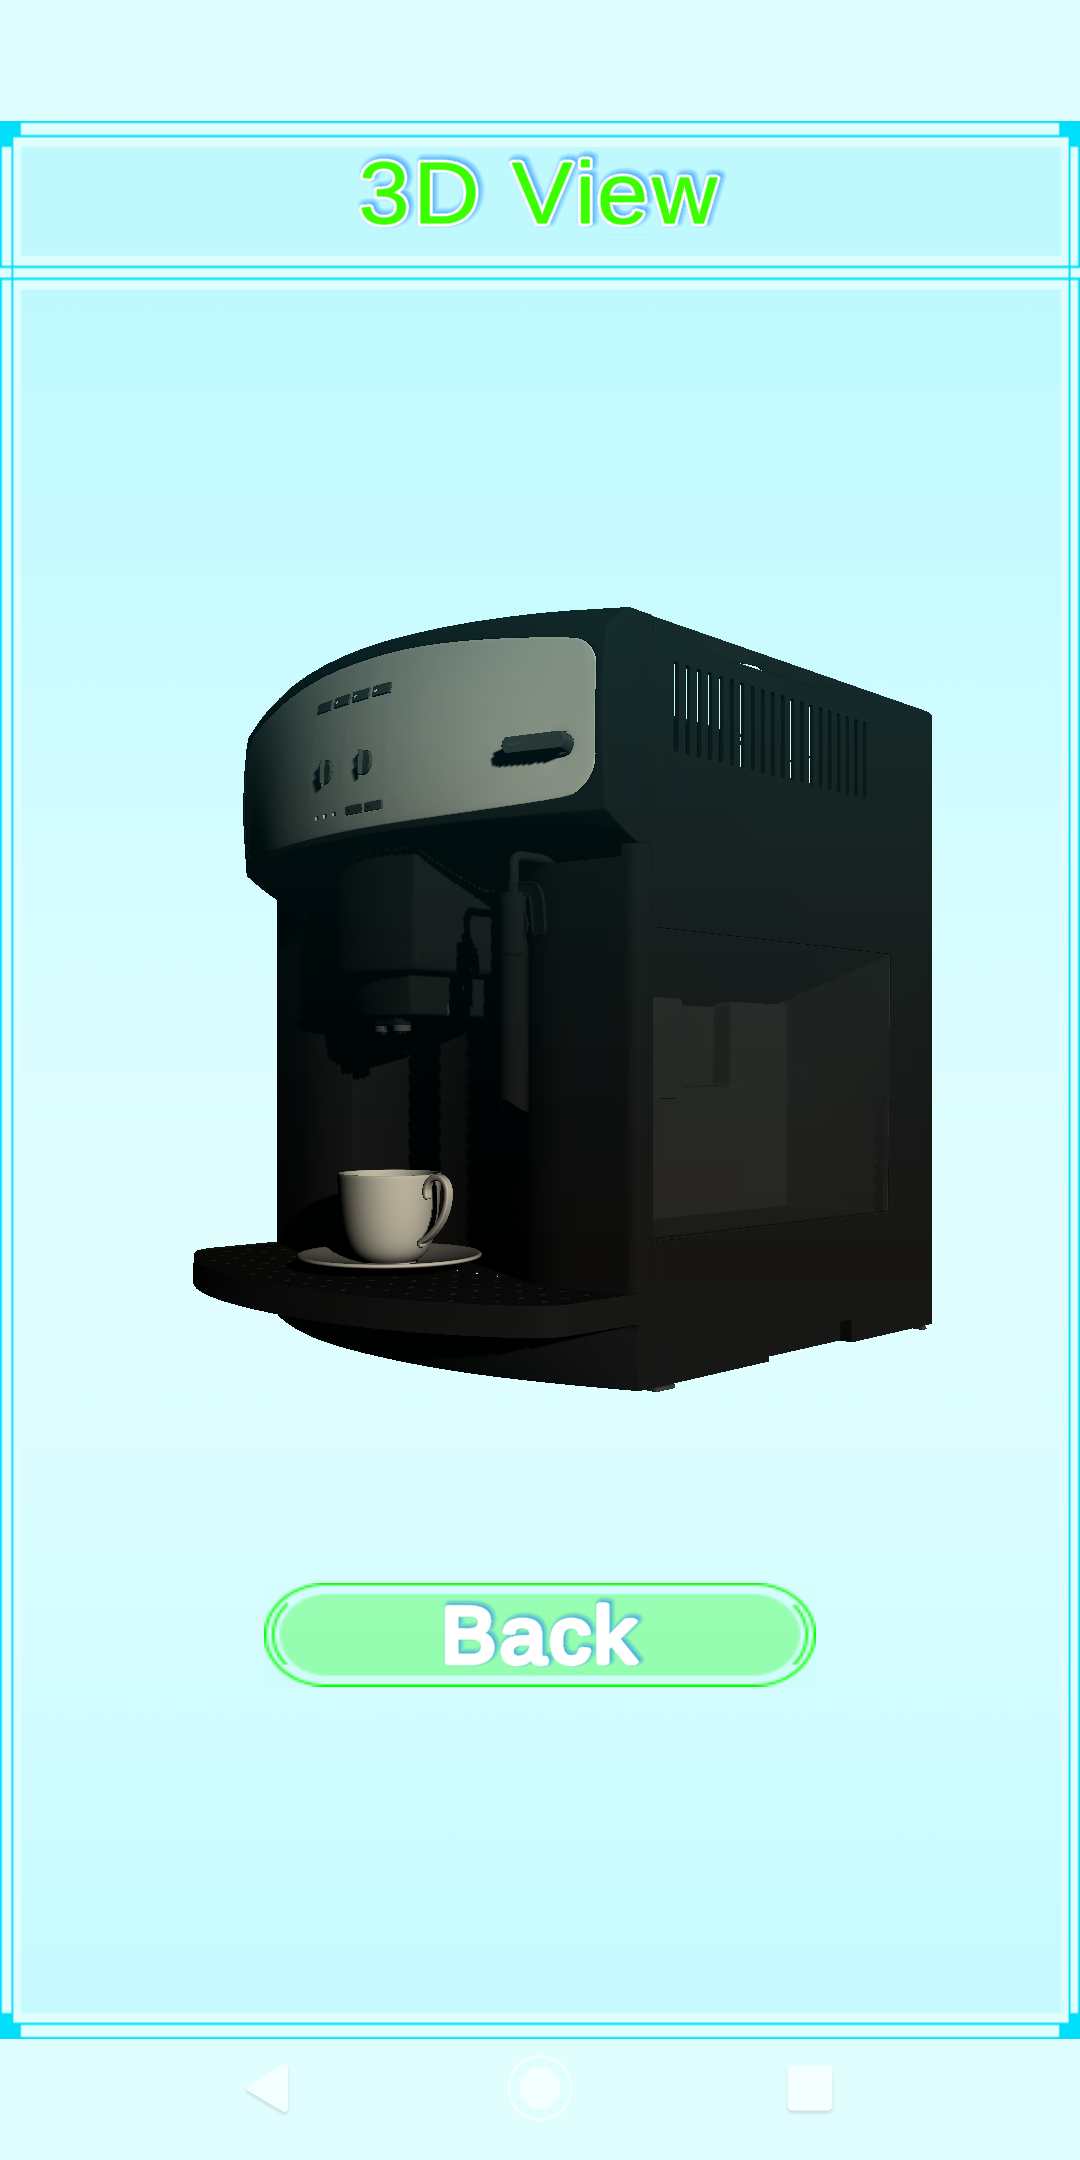
\includegraphics[scale=0.2]{Images/Chapter5/Impl4.png}
          \captionof{figure}{Coffee Machine 3D View}
          \label{fig:CoffeeMachine3D}
        \end{minipage}
\end{figure}
% ///////////////////////////////////////////////////////////////////////////////////////////////////
\section{Image Targets Augmentation Star Rating}
\begin{figure}[H]
    \centering
        \begin{minipage}{.5\textwidth}
          \centering
          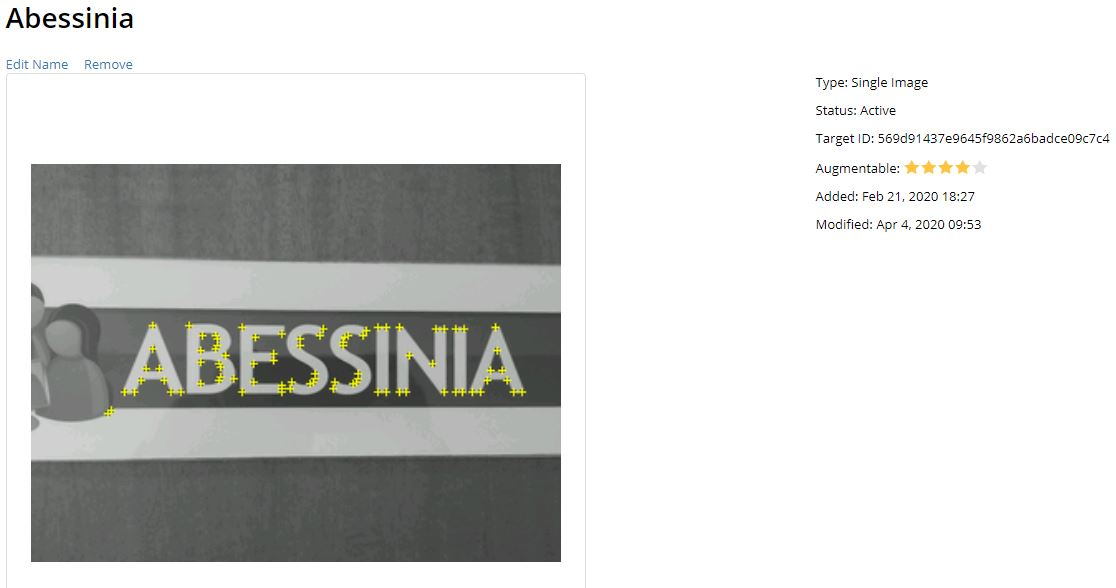
\includegraphics[scale=0.3]{Images/Chapter6/AbessiniaImageTarget.JPG}
          \captionof{figure}{Abessinia Image Target}
          \label{fig:AbessiniaImageTarget}
        \end{minipage}%
        \begin{minipage}{.5\textwidth}
          \centering
          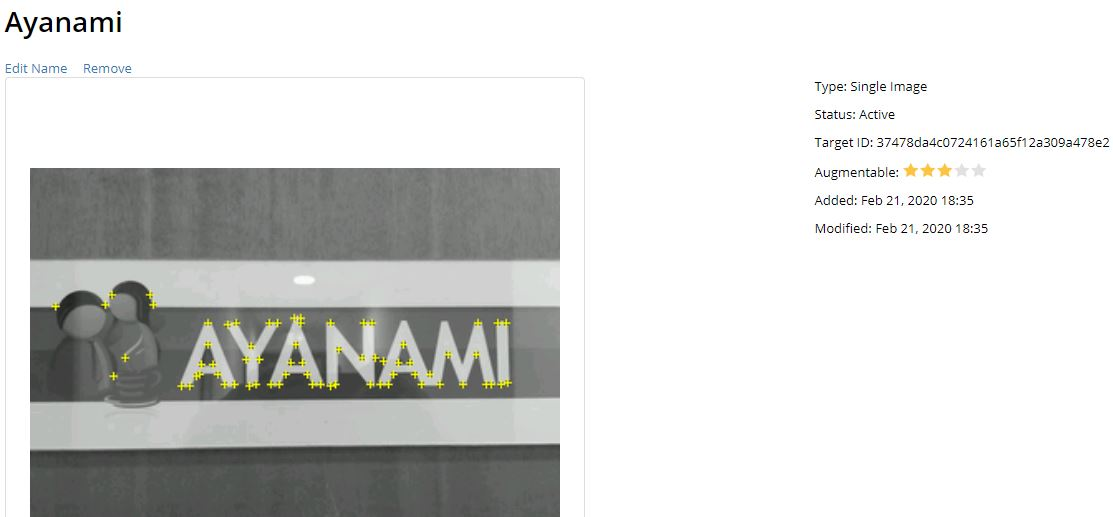
\includegraphics[scale=0.3]{Images/Chapter6/AyanamiImageTarget.JPG}
          \captionof{figure}{Ayanami Image Target}
          \label{fig:AyanamiImageTarget}
        \end{minipage}
\end{figure}
\begin{figure}[H]
    \centering
        \begin{minipage}{.5\textwidth}
          \centering
          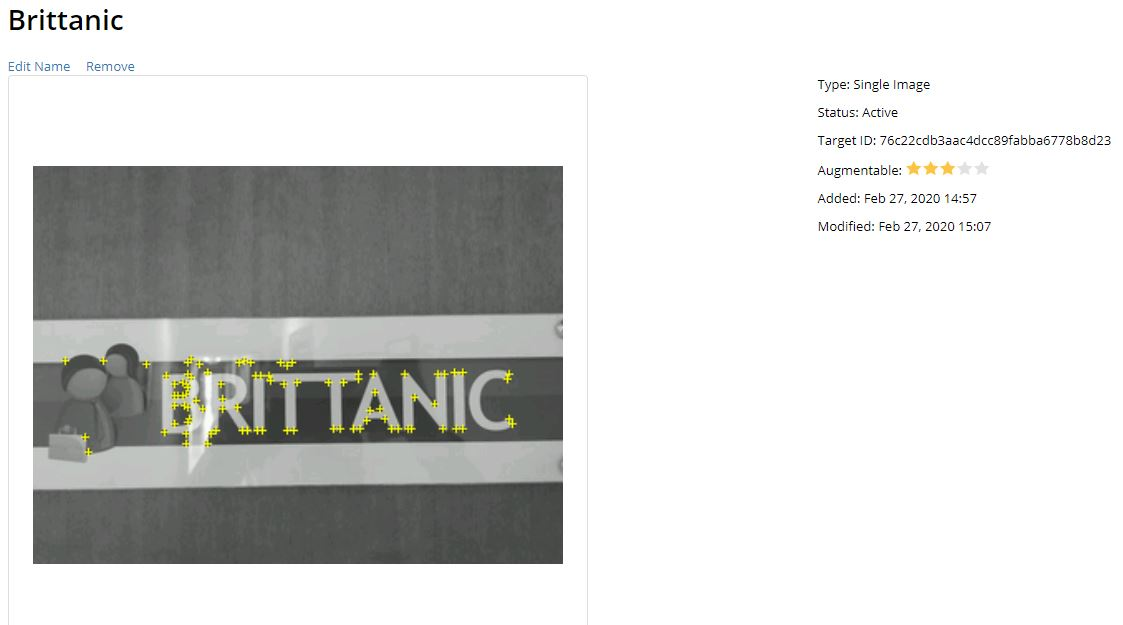
\includegraphics[scale=0.3]{Images/Chapter6/BrittanicImageTargets.JPG}
          \captionof{figure}{Brittanic Image Target}
          \label{fig:BrittanicImageTarget}
        \end{minipage}%
        \begin{minipage}{.5\textwidth}
          \centering
          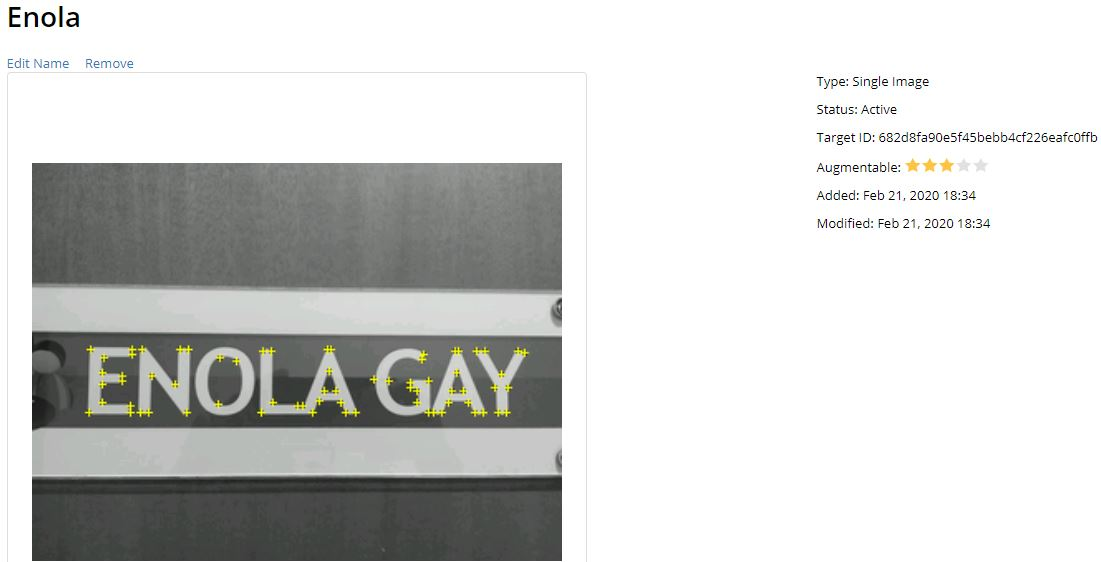
\includegraphics[scale=0.3]{Images/Chapter6/EnolaImageTarget.JPG}
          \captionof{figure}{Enola Image Target}
          \label{fig:EnolaImageTarget}
        \end{minipage}
\end{figure}
\begin{figure}[H]
    \centering
        \begin{minipage}{.5\textwidth}
          \centering
          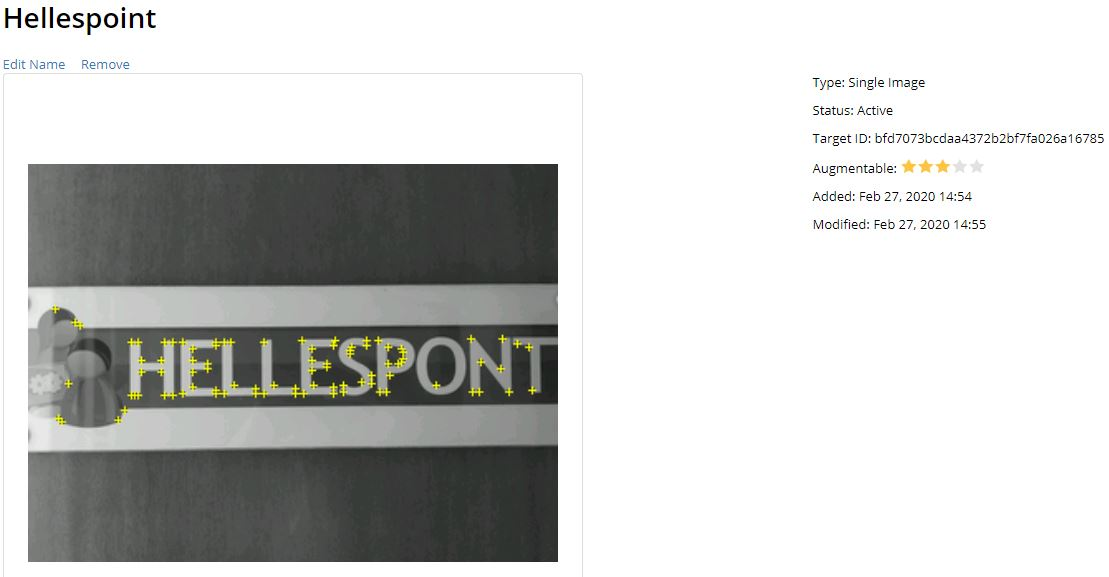
\includegraphics[scale=0.3]{Images/Chapter6/HellespontImageTarget.JPG}
          \captionof{figure}{Hellespont Image Target}
          \label{fig:HellespontImageTarget}
        \end{minipage}%
        \begin{minipage}{.5\textwidth}
          \centering
          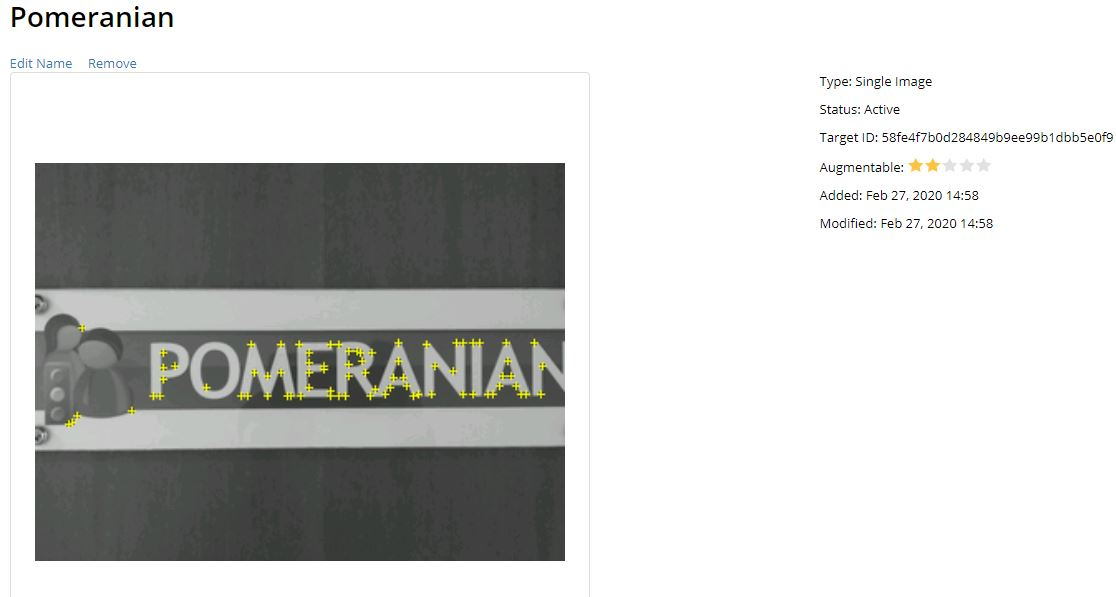
\includegraphics[scale=0.3]{Images/Chapter6/PomeranianImageTarget.JPG}
          \captionof{figure}{Pomeranian Image Target}
          \label{fig:PomeranianImageTarget}
        \end{minipage}
\end{figure}
\begin{figure}[H]
    \centering
        \begin{minipage}{.5\textwidth}
          \centering
          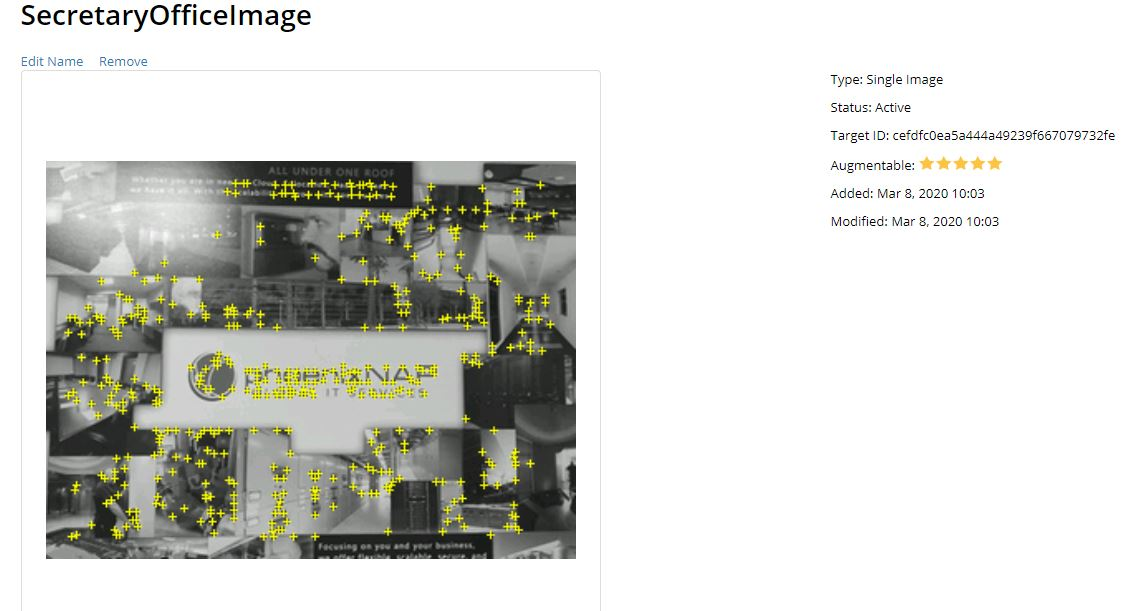
\includegraphics[scale=0.3]{Images/Chapter6/SecretaryImageTarget.JPG}
          \captionof{figure}{Secretary Image Target}
          \label{fig:SecretaryImageTarget}
        \end{minipage}%
        \begin{minipage}{.5\textwidth}
          \centering
          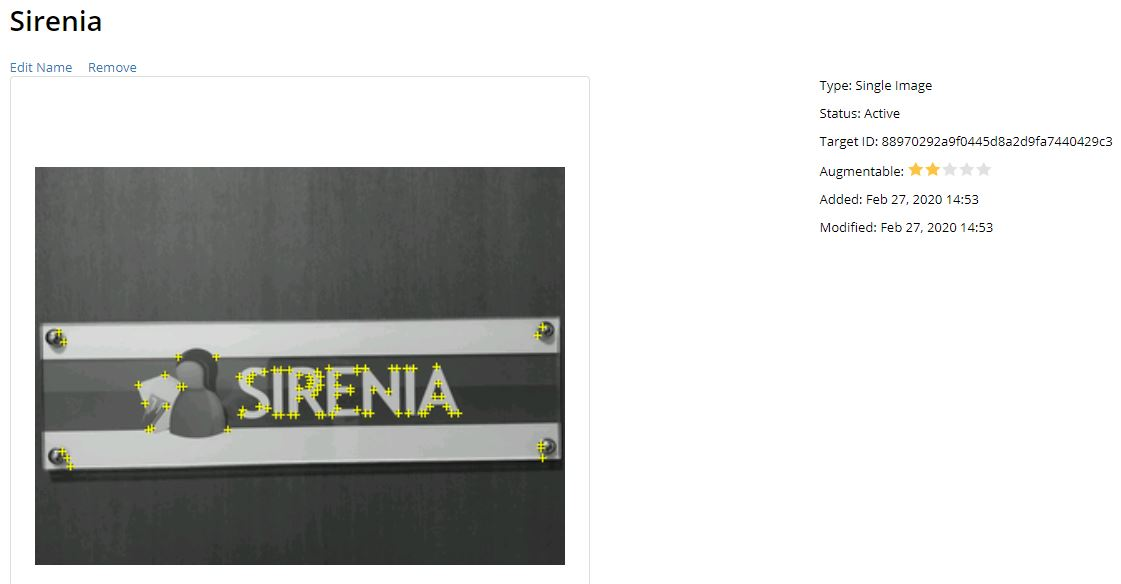
\includegraphics[scale=0.3]{Images/Chapter6/SireniaImageTarget.JPG}
          \captionof{figure}{Sirenia Image Target}
          \label{fig:SireniaImageTarget}
        \end{minipage}
\end{figure}
\begin{figure}[H]
    \centering
        \begin{minipage}{.5\textwidth}
          \centering
          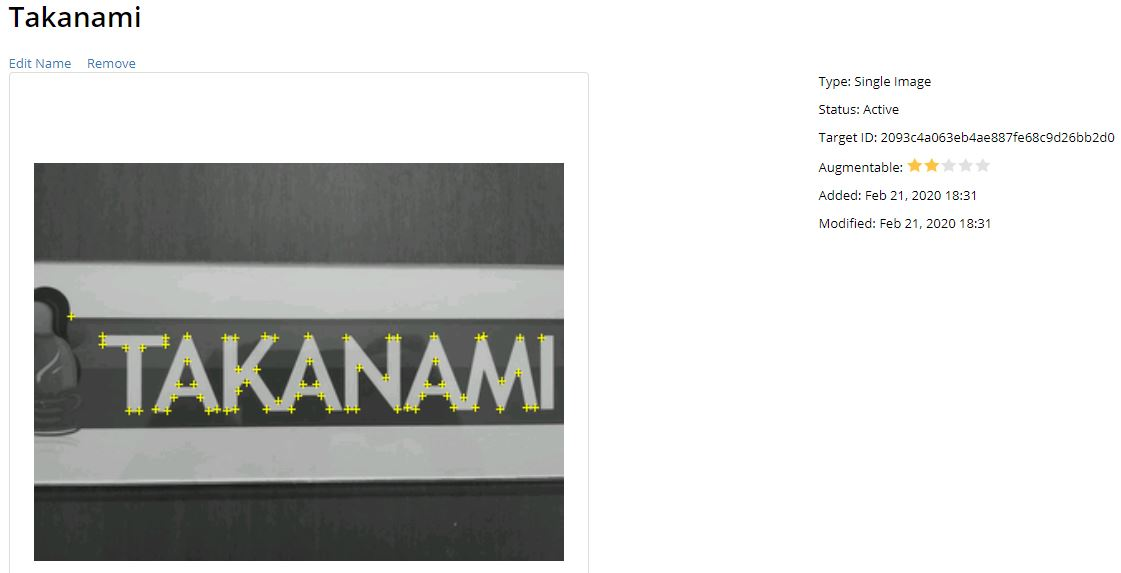
\includegraphics[scale=0.3]{Images/Chapter6/TakanamiImageTarget.JPG}
          \captionof{figure}{Takanami Image Target}
          \label{fig:TakanamiImageTarget}
        \end{minipage}%
        \begin{minipage}{.5\textwidth}
          \centering
          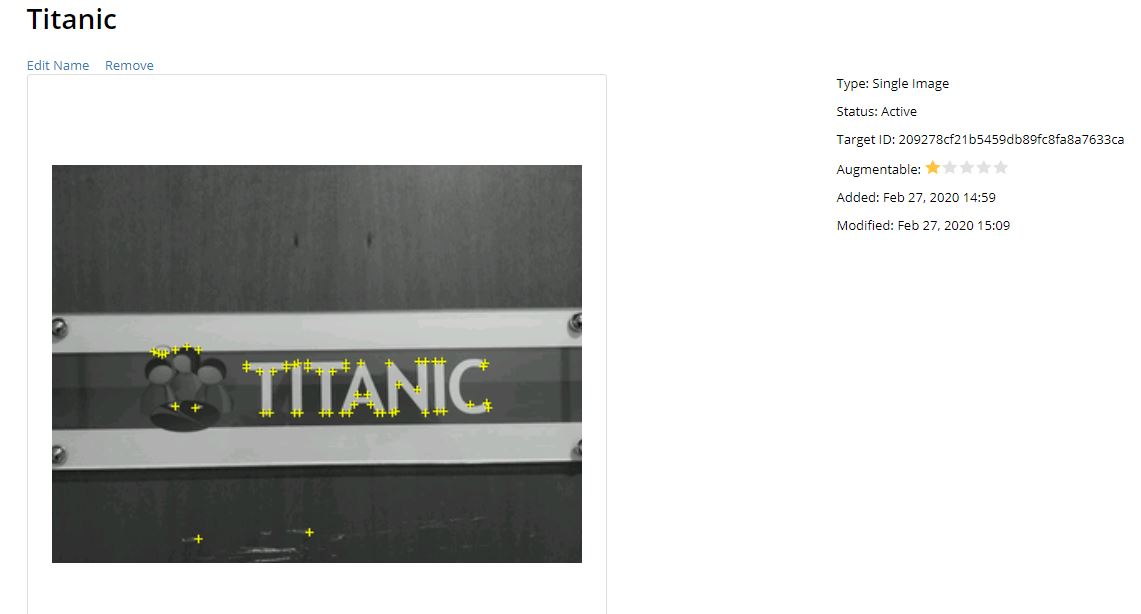
\includegraphics[scale=0.3]{Images/Chapter6/TitanicImageTargets.JPG}
          \captionof{figure}{Titanic Image Target}
          \label{fig:TitanicImageTarget}
        \end{minipage}
\end{figure}
\section{Colour Variance Results (Black and White)}
\begin{figure}[H]
    \centering
    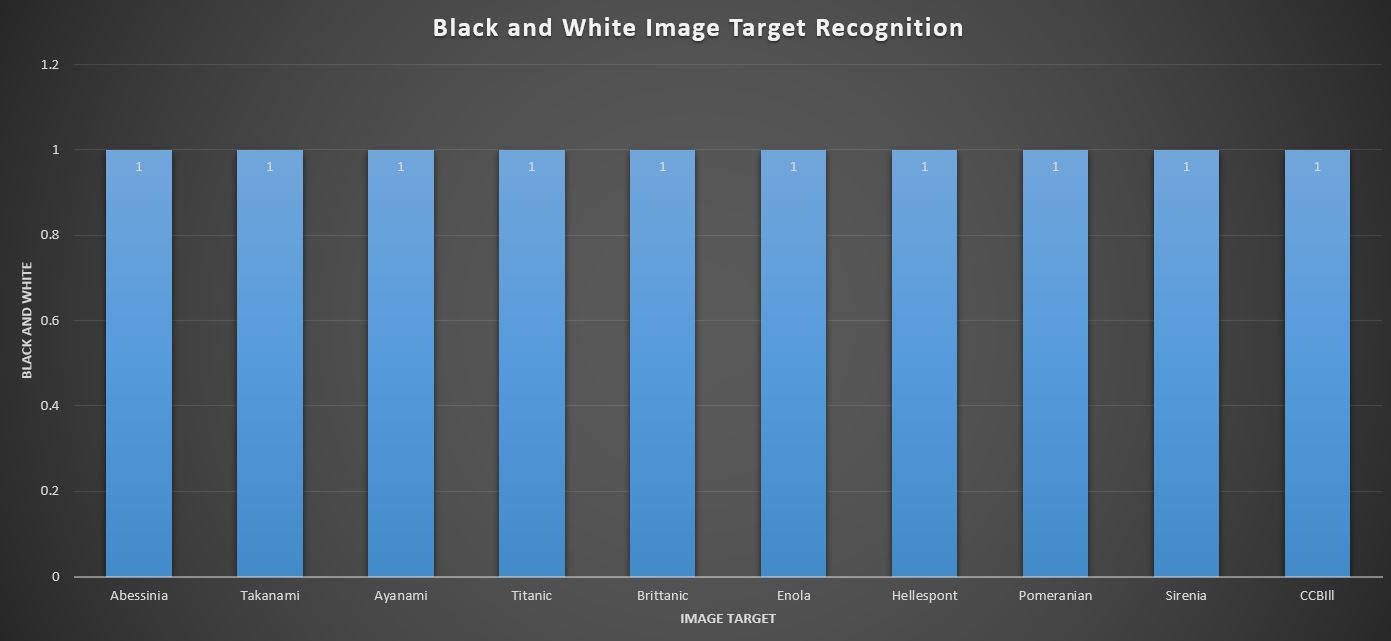
\includegraphics[scale=0.4]{Images/Chapter6/ImageTargetColourVariance.JPG}
    \captionof{figure}{Image Targets' Recognition Strength to Colour (Black and White) Variance Bar Chart}
    \label{fig:ImageTargetColourBarchart}
\end{figure}
\begin{figure}[H]
    \centering
    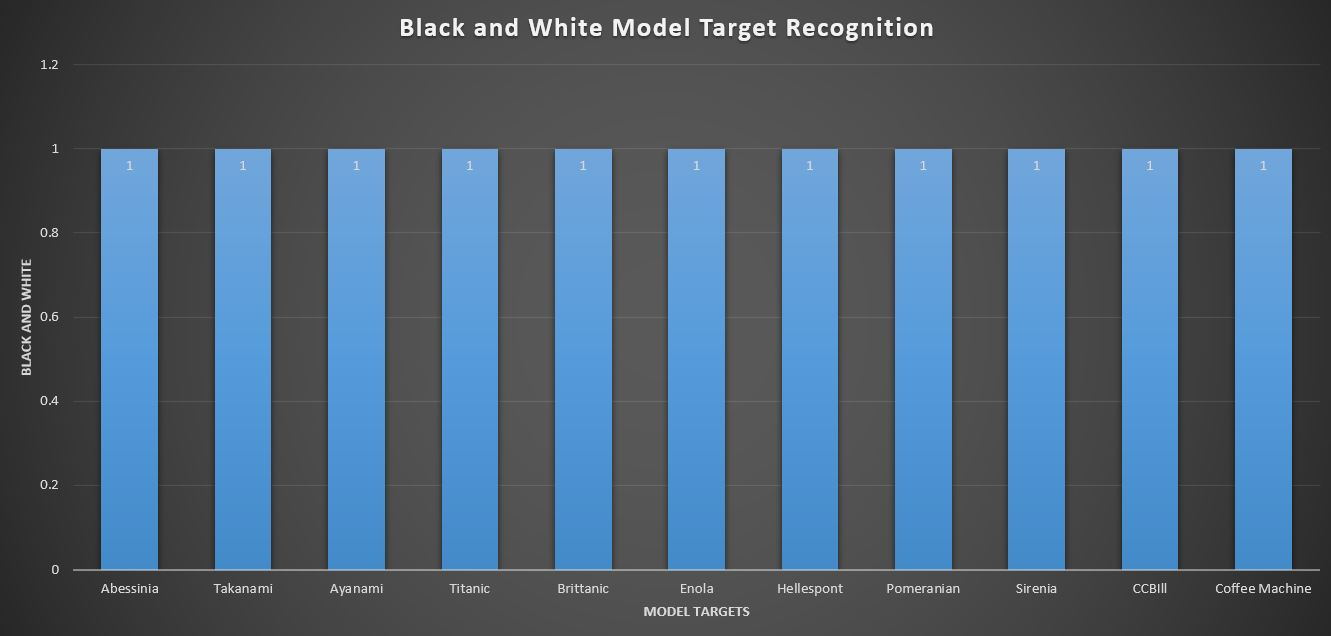
\includegraphics[scale=0.4]{Images/Chapter6/ModelTargetColourVariance.JPG}
    \captionof{figure}{Model Targets' Recognition Strength to Colour (Black and White) Variance Bar Chart}
    \label{fig:ModelTargetColourBarchart}
\end{figure}
\section{Distance Variance Results}
\begin{figure}[H]
    \centering
    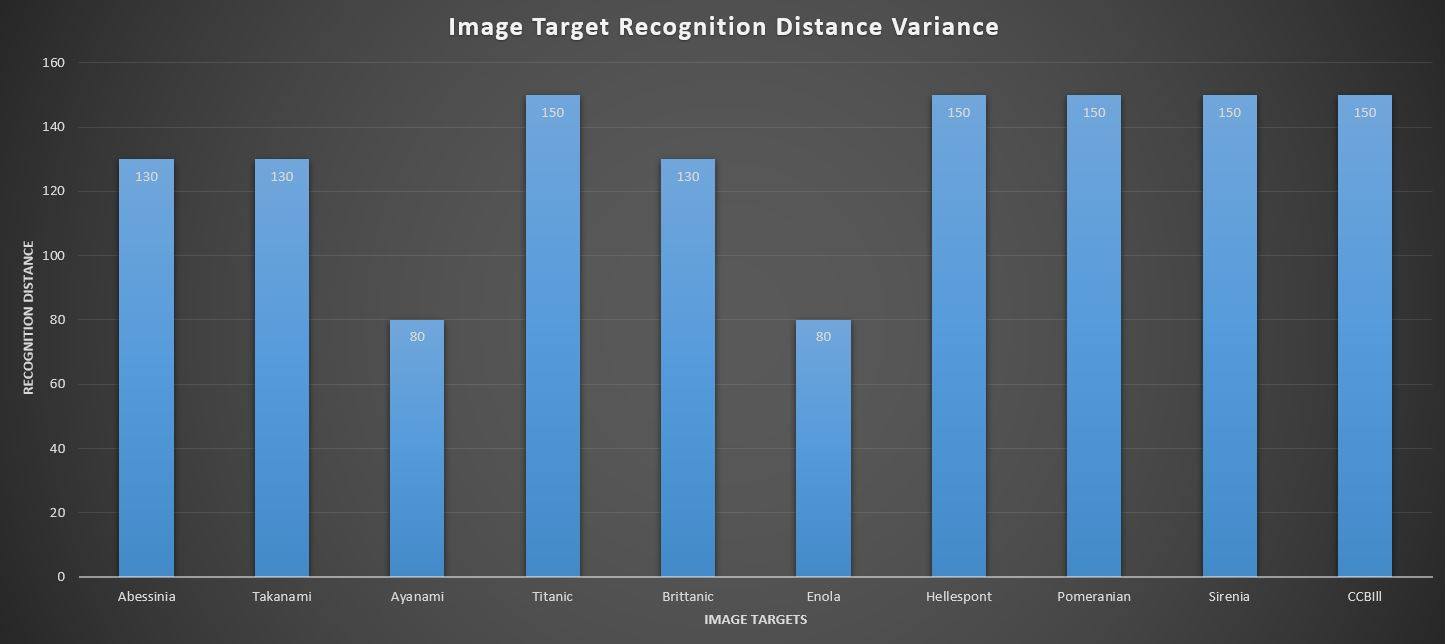
\includegraphics[scale=0.4]{Images/Chapter6/ImageTargetDistanceVairance.JPG}
    \captionof{figure}{Image Targets' Recognition Strength to Distance Variance Bar Chart}
    \label{fig:ImageTargetDistanceBarchart}
\end{figure}
\begin{figure}[H]
    \centering
    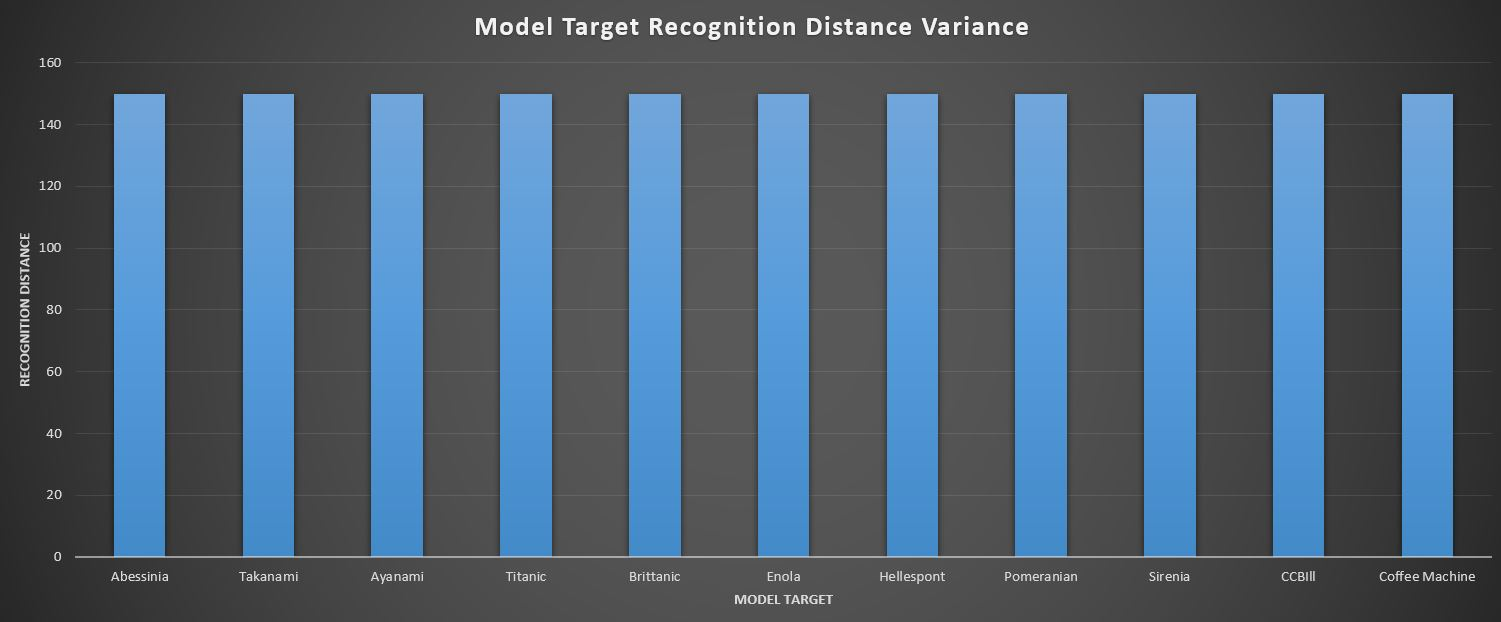
\includegraphics[scale=0.4]{Images/Chapter6/ModelTargetDistanceVariance.JPG}
    \captionof{figure}{Model Targets' Recognition Strength to Distance Variance Bar Chart}
    \label{fig:ModelTargetDistanceBarchart}
\end{figure}
\section{Orientation Variance Results}
\begin{figure}[H]
    \centering
    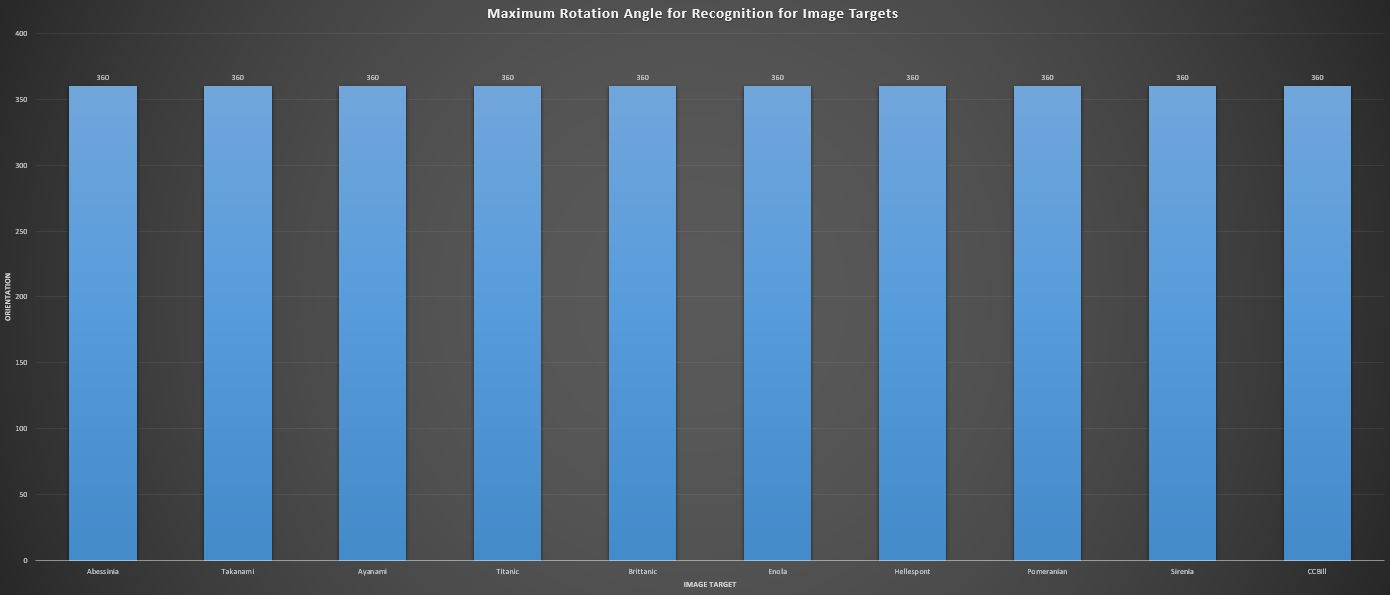
\includegraphics[scale=0.42]{Images/Chapter6/MaximumRotationImageTargets.JPG}
    \captionof{figure}{Image Targets' Recognition Strength to Orientation Variance Bar Chart}
    \label{fig:ImageTargetRotationBarchart}
\end{figure}
\begin{figure}[H]
    \centering
    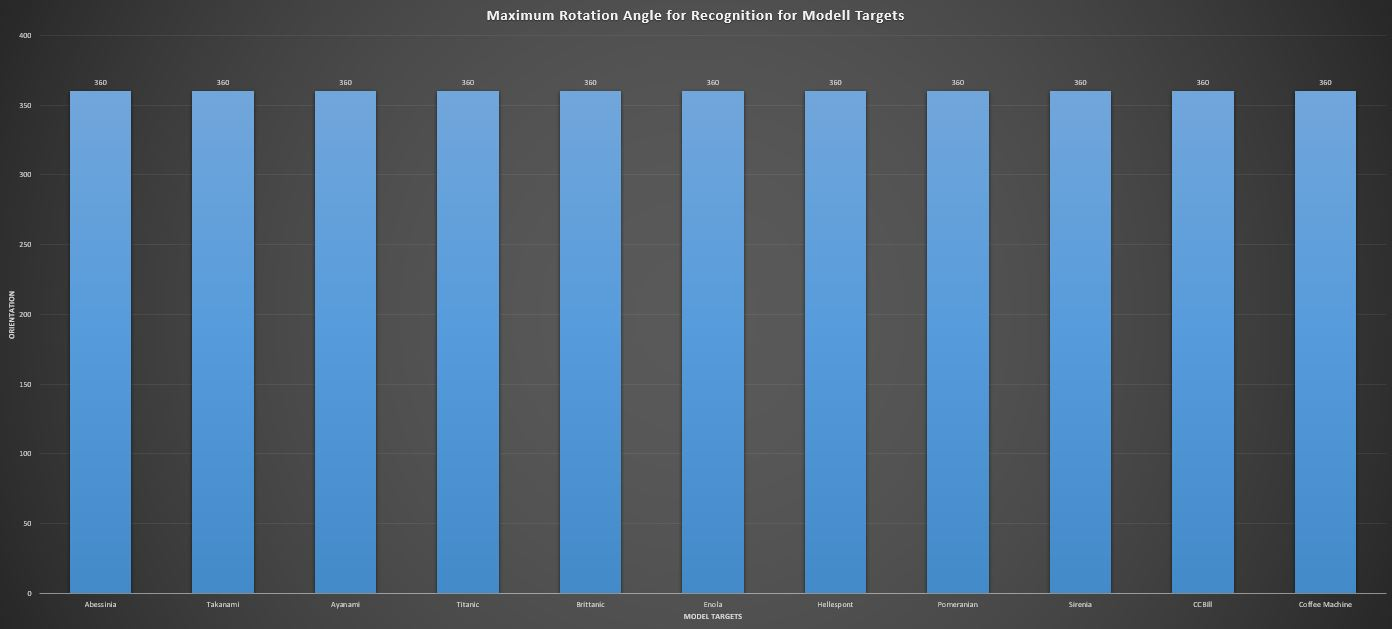
\includegraphics[scale=0.42]{Images/Chapter6/MaximumRotationModelTargets.JPG}
    \captionof{figure}{Model Targets' Recognition Strength to Orientation Variance Bar Chart}
    \label{fig:ModelTargetRotationBarchart}
\end{figure}
\section{Occlusion Variance Results}
\begin{figure}[H]
    \centering
    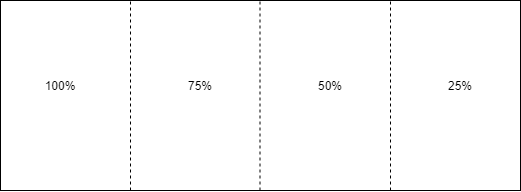
\includegraphics[scale=0.7]{Images/Chapter6/ImageOcclusion.png}
    \captionof{figure}{Marker's Occlusion Percentages}
    \label{fig:ImageOcclusionPercentages}
\end{figure}
\begin{figure}[H]
    \centering
    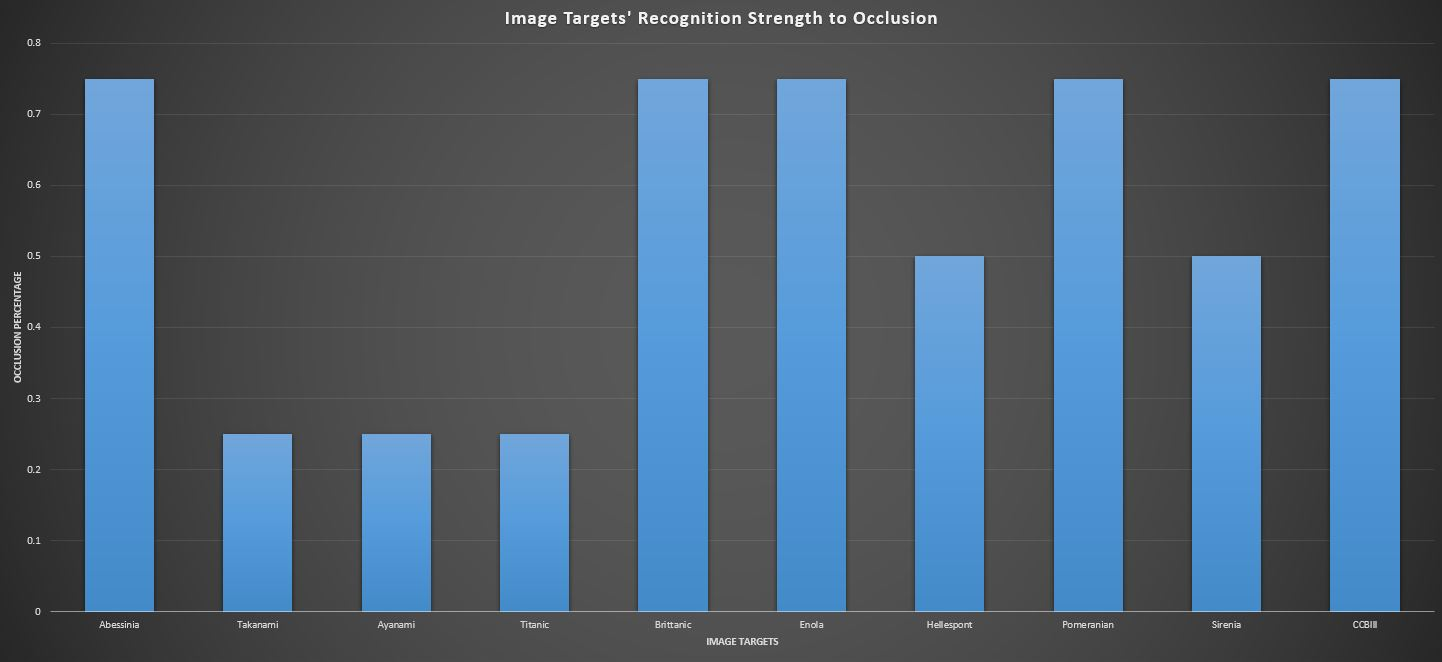
\includegraphics[scale=0.4]{Images/Chapter6/OcclusionImageTargetStrenghtBarChart.JPG}
    \captionof{figure}{Image Targets' Recognition Strength to Occlusion Bar Chart}
    \label{fig:ImageTargetOcclusionBarchart}
\end{figure}
\begin{figure}[H]
    \centering
    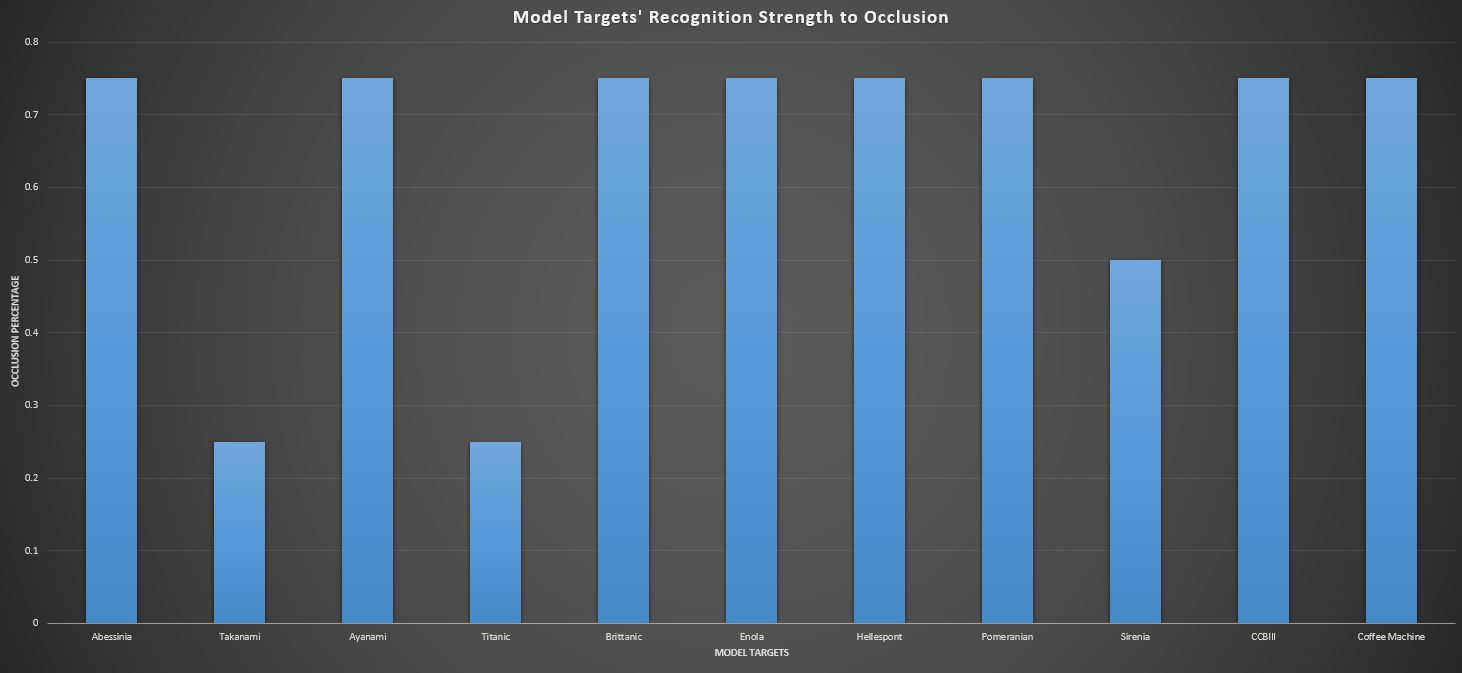
\includegraphics[scale=0.4]{Images/Chapter6/OcclusionModelTargetStrenghtBarChart.JPG}
    \captionof{figure}{Model Targets' Recognition Strength to Occlusion Bar Chart}
    \label{fig:ModelTargetOcclusionBarchart}
\end{figure}

\newpage
\section{User-Tasks Ratings Distribution Plots}
\begin{figure}[H]
    \centering
    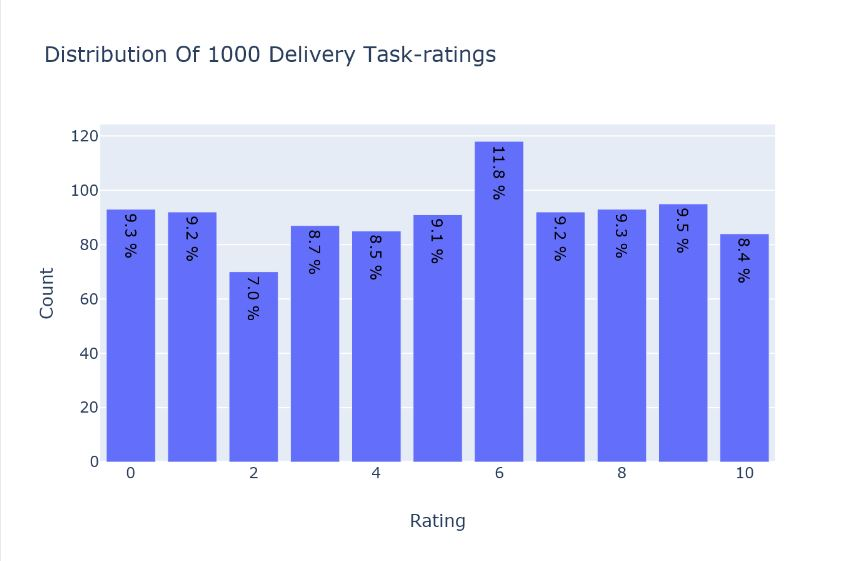
\includegraphics[scale=0.5]{Images/Chapter6/DistDelivRatings.JPG}
    \captionof{figure}{Distribution of 1000 Delivery Task-Ratings Barchart}
    \label{fig:DistDeliveryRatingsBarchart}
\end{figure}
\begin{figure}[H]
    \centering
    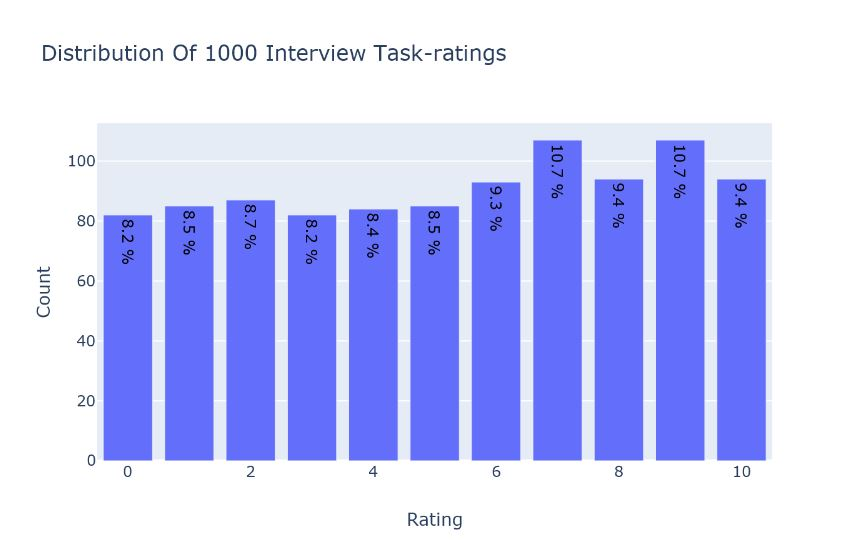
\includegraphics[scale=0.5]{Images/Chapter6/DistIntRatings.JPG}
    \captionof{figure}{Distribution of 1000 Interview Task-Ratings Barchart}
    \label{fig:DistIntRatingsBarchart}
\end{figure}
\begin{figure}[H]
    \centering
    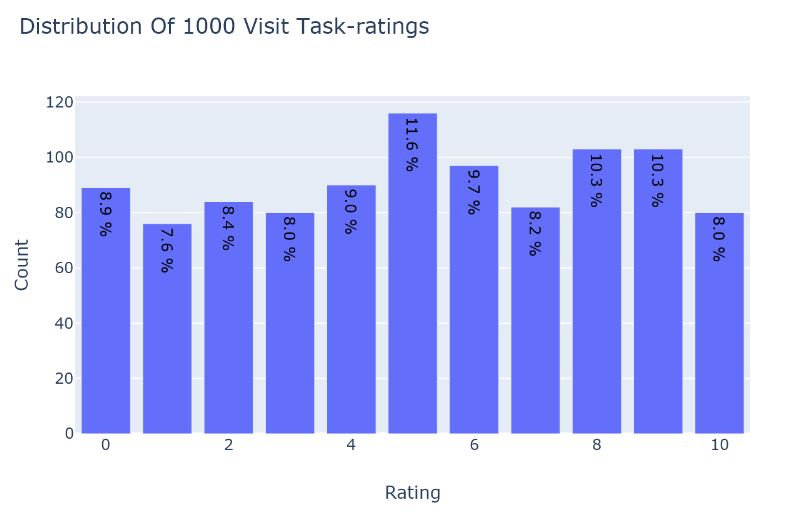
\includegraphics[scale=0.5]{Images/Chapter6/DistvisitRatings.JPG}
    \captionof{figure}{Distribution of 1000 Visit Task-Ratings Barchart}
    \label{fig:DistVisitRatingsBarchart}
\end{figure}
\begin{figure}[H]
    \centering
    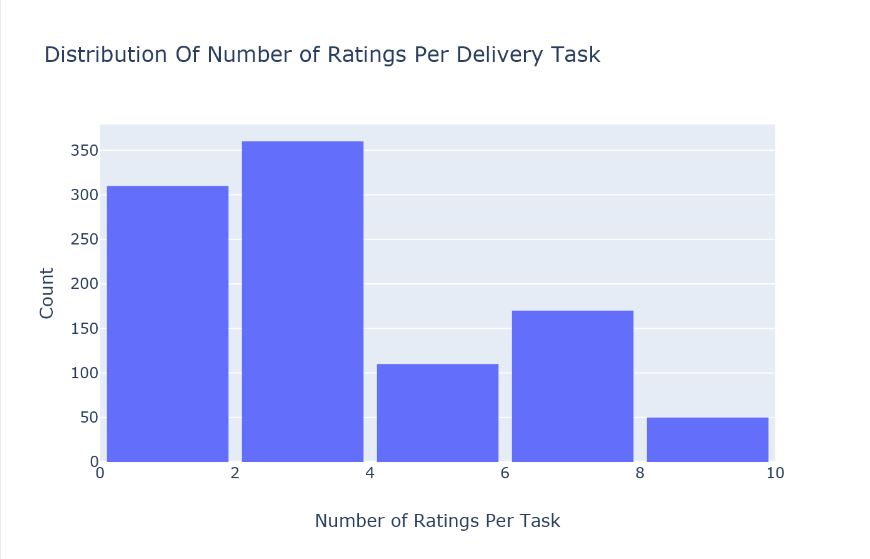
\includegraphics[scale=0.5]{Images/Chapter6/DistofNumofDelivRatingPerTask.JPG}
    \captionof{figure}{Distribution of Number of Ratings Per Delivery Task Barchart}
    \label{fig:DistNumRatingPerDeliveryBarchart}
\end{figure}
\begin{figure}[H]
    \centering
    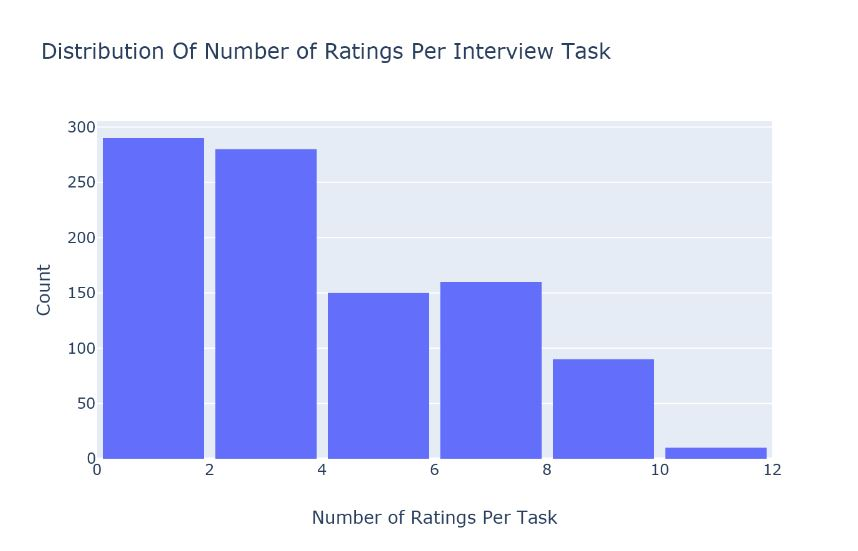
\includegraphics[scale=0.5]{Images/Chapter6/DistofNumofIntRatingPerTask.JPG}
    \captionof{figure}{Distribution of Number of Ratings Per Interview Task Barchart}
    \label{fig:DistNumRatingPerInterviewBarchart}
\end{figure}
\begin{figure}[H]
    \centering
    \includegraphics[scale=0.5]{Images/Chapter6/DistofNumofVisitRatingPerTask.JPG}
    \captionof{figure}{Distribution of Number of Ratings Per Visit Task Barchart}
    \label{fig:DistNumRatingPerVisitBarchart}
\end{figure}
\begin{figure}[H]
    \centering
    \includegraphics[scale=0.5]{Images/Chapter6/DistributionofRatingsPerUserDeliv.JPG}
    \captionof{figure}{Distribution of Delivery Ratings Per User Barchart}
    \label{fig:DistDelivRatingPerUserBarchart}
\end{figure}
\begin{figure}[H]
    \centering
    \includegraphics[scale=0.5]{Images/Chapter6/DistributionofRatingsPerUserInt.JPG}
    \captionof{figure}{Distribution of Interview Ratings Per User Barchart}
    \label{fig:DistIntRatingPerUserBarchart}
\end{figure}
\begin{figure}[H]
    \centering
    \includegraphics[scale=0.5]{Images/Chapter6/DistributionofRatingsPerUserVisit.JPG}
    \captionof{figure}{Distribution of Visit Ratings Per User Barchart}
    \label{fig:DistVisitRatingPerUserBarchart}
\end{figure}

\newpage
\section{Recommendation Models Comparison on RMSE and MAE Values}
\begin{figure}[H]
    \centering
    \includegraphics[scale=0.7]{Images/Chapter6/Plot9Delivery.JPG}
    \captionof{figure}{Comparison of Algorithms on RMSE and MAE for Delivery}
    \label{fig:Plot9Delivery}
\end{figure}
\begin{figure}[H]
    \centering
    \includegraphics[scale=0.7]{Images/Chapter6/Plot9Interview.JPG}
    \captionof{figure}{Comparison of Algorithms on RMSE and MAE for Interview}
    \label{fig:Plot9Interview}
\end{figure}
\begin{figure}[H]
    \centering
    \includegraphics[scale=0.7]{Images/Chapter6/PlotVisit.JPG}
    \captionof{figure}{Comparison of Algorithms on RMSE and MAE for Visit}
    \label{fig:Plot9Visit}
\end{figure}
\begin{figure}[H]
    \centering
    \includegraphics[scale=0.4]{Images/Chapter6/MeanRMSE.JPG}
    \captionof{figure}{Comparison of Algorithms on Average RMSE for Visit, Interview and Delivery}
    \label{fig:AverageRMSEALL}
\end{figure}
\begin{figure}[H]
    \centering
    \includegraphics[scale=0.4]{Images/Chapter6/MeanMAE.JPG}
    \captionof{figure}{Comparison of Algorithms on Average MAE for Visit, Interview and Delivery}
    \label{fig:AverageMAEALL}
\end{figure}

\newpage
\section{Qualitative Evaluation Results}
\begin{figure}[H]
    \centering
    \includegraphics[scale=0.4]{Images/Chapter6/UserEvaluation/Total/ParticipantsPiechar.JPG}
    \captionof{figure}{Participants (Employees and Visitors)}
    \label{fig:figure1}
\end{figure}

\begin{figure}[H]\centering
\subfloat[Combined]{\label{a}\includegraphics[scale=.4]{Images/Chapter6/UserEvaluation/Total/Figure4Comb.JPG}}\par
\subfloat[CCBill Participants]{\label{b}\includegraphics[width=.45\linewidth]{Images/Chapter6/UserEvaluation/CCBill/Figure3CCbill.JPG}}\hfill 
\subfloat[Non-CCBill Participants]{\label{c}\includegraphics[width=.45\linewidth]{Images/Chapter6/UserEvaluation/NonCCbill/Figure3Nonccbill.JPG}}
\caption{Survey: Question 1 }
\label{fig:figure2}
\end{figure}
\begin{figure}[H]\centering
\subfloat[Combined]{\label{a}\includegraphics[scale=.4]{Images/Chapter6/UserEvaluation/Total/Figure5Comb.JPG}}\par
\subfloat[CCBill Participants]{\label{b}\includegraphics[width=.45\linewidth]{Images/Chapter6/UserEvaluation/CCBill/Figure4CCbill.JPG}}\hfill 
\subfloat[Non-CCBill Participants]{\label{c}\includegraphics[width=.45\linewidth]{Images/Chapter6/UserEvaluation/NonCCbill/Figure4Nonccbill.JPG}}
\caption{Survey: Question 2 }
\label{fig:figure3}
\end{figure}
\begin{figure}[H]\centering
\subfloat[Combined]{\label{a}\includegraphics[scale=.4]{Images/Chapter6/UserEvaluation/Total/Figure6Comb.JPG}}\par
\subfloat[CCBill Participants]{\label{b}\includegraphics[width=.45\linewidth]{Images/Chapter6/UserEvaluation/CCBill/Figure5CCbill.JPG}}\hfill 
\subfloat[Non-CCBill Participants]{\label{c}\includegraphics[width=.45\linewidth]{Images/Chapter6/UserEvaluation/NonCCbill/Figure5Nonccbill.JPG}}
\caption{Survey: Question 3 }
\label{fig:figure4}
\end{figure}
\begin{figure}[H]\centering
\subfloat[Combined]{\label{a}\includegraphics[scale=.4]{Images/Chapter6/UserEvaluation/Total/Figure7Comb.JPG}}\par
\subfloat[CCBill Participants]{\label{b}\includegraphics[width=.45\linewidth]{Images/Chapter6/UserEvaluation/CCBill/Figure6CCbill.JPG}}\hfill 
\subfloat[Non-CCBill Participants]{\label{c}\includegraphics[width=.45\linewidth]{Images/Chapter6/UserEvaluation/NonCCbill/Figure6Nonccbill.JPG}}
\caption{Survey: Question 4 }
\label{fig:figure5}
\end{figure}
\begin{figure}[H]\centering
\subfloat[Combined]{\label{a}\includegraphics[scale=.4]{Images/Chapter6/UserEvaluation/Total/User-Friendly.JPG}}\par
\subfloat[CCBill Participants]{\label{b}\includegraphics[width=.45\linewidth]{Images/Chapter6/UserEvaluation/CCBill/Figure7CCbill.JPG}}\hfill 
\subfloat[Non-CCBill Participants]{\label{c}\includegraphics[width=.45\linewidth]{Images/Chapter6/UserEvaluation/NonCCbill/Figure7Nonccbill.JPG}}
\caption{Survey: Question 5 }
\label{fig:figure6}
\end{figure}
\begin{figure}[H]\centering
\subfloat[Combined]{\label{a}\includegraphics[scale=.4]{Images/Chapter6/UserEvaluation/Total/Figure16Comb.JPG}}\par
\subfloat[CCBill Participants]{\label{b}\includegraphics[width=.45\linewidth]{Images/Chapter6/UserEvaluation/CCBill/Figure15.JPG}}\hfill 
\subfloat[Non-CCBill Participants]{\label{c}\includegraphics[width=.45\linewidth]{Images/Chapter6/UserEvaluation/NonCCbill/Figure15nonccbill.JPG}}
\caption{Survey: Question 6 }
\label{fig:figure7}
\end{figure}
\begin{figure}[H]\centering
\subfloat[Combined]{\label{a}\includegraphics[scale=.4]{Images/Chapter6/UserEvaluation/Total/Figure9Comb.JPG}}\par
\subfloat[CCBill Participants]{\label{b}\includegraphics[width=.45\linewidth]{Images/Chapter6/UserEvaluation/CCBill/Figure8CCbill.JPG}}\hfill 
\subfloat[Non-CCBill Participants]{\label{c}\includegraphics[width=.45\linewidth]{Images/Chapter6/UserEvaluation/NonCCbill/Figure8nonccbill.JPG}}
\caption{Survey: Question 7 }
\label{fig:figure8}
\end{figure}
\begin{figure}[H]\centering
\subfloat[Combined]{\label{a}\includegraphics[scale=.4]{Images/Chapter6/UserEvaluation/Total/Figure17Comb.JPG}}\par
\subfloat[CCBill Participants]{\label{b}\includegraphics[width=.45\linewidth]{Images/Chapter6/UserEvaluation/CCBill/Figure16.JPG}}\hfill 
\subfloat[Non-CCBill Participants]{\label{c}\includegraphics[width=.45\linewidth]{Images/Chapter6/UserEvaluation/NonCCbill/Figure16nonccbill.JPG}}
\caption{Survey: Question 8 }
\label{fig:figure9}
\end{figure}
\begin{figure}[H]\centering
\subfloat[Combined]{\label{a}\includegraphics[scale=.4]{Images/Chapter6/UserEvaluation/Total/Figure10Comb.JPG}}\par
\subfloat[CCBill Participants]{\label{b}\includegraphics[width=.45\linewidth]{Images/Chapter6/UserEvaluation/CCBill/Figure9CCbill.JPG}}\hfill 
\subfloat[Non-CCBill Participants]{\label{c}\includegraphics[width=.45\linewidth]{Images/Chapter6/UserEvaluation/NonCCbill/Figure9nonccbill.JPG}}
\caption{Survey: Question 9 }
\label{fig:figure10}
\end{figure}
\begin{figure}[H]\centering
\subfloat[Combined]{\label{a}\includegraphics[scale=.4]{Images/Chapter6/UserEvaluation/Total/Figure11Comb.JPG}}\par
\subfloat[CCBill Participants]{\label{b}\includegraphics[width=.45\linewidth]{Images/Chapter6/UserEvaluation/CCBill/Figure10CCbill.JPG}}\hfill 
\subfloat[Non-CCBill Participants]{\label{c}\includegraphics[width=.45\linewidth]{Images/Chapter6/UserEvaluation/NonCCbill/Figure10nonccbill.JPG}}
\caption{Survey: Question 10 }
\label{fig:figure11}
\end{figure}
\begin{figure}[H]\centering
\subfloat[Combined]{\label{a}\includegraphics[scale=.4]{Images/Chapter6/UserEvaluation/Total/Figure12Comb.JPG}}\par
\subfloat[CCBill Participants]{\label{b}\includegraphics[width=.45\linewidth]{Images/Chapter6/UserEvaluation/CCBill/Figure11CCbill.JPG}}\hfill 
\subfloat[Non-CCBill Participants]{\label{c}\includegraphics[width=.45\linewidth]{Images/Chapter6/UserEvaluation/NonCCbill/Figure11nonccbill.JPG}}
\caption{Survey: Question 11 }
\label{fig:figure12}
\end{figure}
\begin{figure}[H]\centering
\subfloat[Combined]{\label{a}\includegraphics[scale=.4]{Images/Chapter6/UserEvaluation/Total/Figure13Comb.JPG}}\par
\subfloat[CCBill Participants]{\label{b}\includegraphics[width=.45\linewidth]{Images/Chapter6/UserEvaluation/CCBill/Figure12CCbill.JPG}}\hfill 
\subfloat[Non-CCBill Participants]{\label{c}\includegraphics[width=.45\linewidth]{Images/Chapter6/UserEvaluation/NonCCbill/Figure12nonccbill.JPG}}
\caption{Survey: Question 12 }
\label{fig:figure13}
\end{figure}
\begin{figure}[H]\centering
\subfloat[Combined]{\label{a}\includegraphics[scale=.4]{Images/Chapter6/UserEvaluation/Total/Figure14Comb.JPG}}\par
\subfloat[CCBill Participants]{\label{b}\includegraphics[width=.45\linewidth]{Images/Chapter6/UserEvaluation/CCBill/Figure13CCbill.JPG}}\hfill 
\subfloat[Non-CCBill Participants]{\label{c}\includegraphics[width=.45\linewidth]{Images/Chapter6/UserEvaluation/NonCCbill/Figure13nonccbill.JPG}}
\caption{Survey: Question 13 }
\label{fig:figure14}
\end{figure}
\begin{figure}[H]\centering
\subfloat[Combined]{\label{a}\includegraphics[scale=.4]{Images/Chapter6/UserEvaluation/Total/Figure15Comb.JPG}}\par
\subfloat[CCBill Participants]{\label{b}\includegraphics[width=.45\linewidth]{Images/Chapter6/UserEvaluation/CCBill/Figure14CCbill.JPG}}\hfill 
\subfloat[Non-CCBill Participants]{\label{c}\includegraphics[width=.45\linewidth]{Images/Chapter6/UserEvaluation/NonCCbill/Figure14nonccbill.JPG}}
\caption{Survey: Question 14 }
\label{fig:figure15}
\end{figure}
\begin{figure}[H]\centering
\subfloat[Combined]{\label{a}\includegraphics[scale=.4]{Images/Chapter6/UserEvaluation/Total/Figure18Comb.JPG}}\par
\subfloat[CCBill Participants]{\label{b}\includegraphics[width=.45\linewidth]{Images/Chapter6/UserEvaluation/CCBill/Figure17.JPG}}\hfill 
\subfloat[Non-CCBill Participants]{\label{c}\includegraphics[width=.45\linewidth]{Images/Chapter6/UserEvaluation/NonCCbill/Figure17nonccbill.JPG}}
\caption{Survey: Question 15 }
\label{fig:figure16}
\end{figure}

% ///////////////////////////////////////////////////////////////////////////////////////////////////
\section{Future Work}
\begin{figure}[H]
    \centering
    \includegraphics[scale=0.2]{Images/Chapter7/futureImpl.png}
    \captionof{figure}{Holographic Corridor Augmentations }
    \label{fig:HolographicArrowsInCorridor}
\end{figure}

\section{Ethics Form}
\includegraphics[scale=0.8]{Forms/EthicsForm.pdf}
\includepdf[pages={2-},scale=0.8]{Forms/EthicsForm.pdf}
% \includepdf[pages=-,pagecommand={},scale=0.1]{Forms/EthicsForm.pdf}
\includepdf[pages=-,pagecommand={},width=\textwidth]{Forms/CCBillConsentEthicsForm.pdf}
\includepdf[pages=-,pagecommand={},width=\textwidth]{Forms/CCBillParticipants/AndrewJr.pdf}
\includepdf[pages=-,pagecommand={},width=\textwidth]{Forms/CCBillParticipants/Bjan.pdf}
\includepdf[pages=-,pagecommand={},width=\textwidth]{Forms/CCBillParticipants/Chris.pdf}
\includepdf[pages=-,pagecommand={},width=\textwidth]{Forms/CCBillParticipants/Cindy.pdf}
\includepdf[pages=-,pagecommand={},width=\textwidth]{Forms/CCBillParticipants/Jake.pdf}
\includepdf[pages=-,pagecommand={},width=\textwidth]{Forms/CCBillParticipants/Joanna.pdf}
\includepdf[pages=-,pagecommand={},width=\textwidth]{Forms/CCBillParticipants/Lara.pdf}
\includepdf[pages=-,pagecommand={},width=\textwidth]{Forms/CCBillParticipants/Leon.pdf}
\includepdf[pages=-,pagecommand={},width=\textwidth]{Forms/CCBillParticipants/Mat.pdf}
\includepdf[pages=-,pagecommand={},width=\textwidth]{Forms/CCBillParticipants/Naeem.pdf}
\includepdf[pages=-,pagecommand={},width=\textwidth]{Forms/CCBillParticipants/Saviour.pdf}
\includepdf[pages=-,pagecommand={},width=\textwidth]{Forms/CCBillParticipants/Steph.pdf}
\includepdf[pages=-,pagecommand={},width=\textwidth]{Forms/CCBillParticipants/Valerio.pdf}
\includepdf[pages=-,pagecommand={},width=\textwidth]{Forms/CCBillParticipants/Zak.pdf}
% --------------------------------------------------------------------------------------------
\includepdf[pages=-,pagecommand={},width=\textwidth]{Forms/NonCCbillParticipants/Ana.pdf}
\includepdf[pages=-,pagecommand={},width=\textwidth]{Forms/NonCCbillParticipants/Andrew.pdf}
\includepdf[pages=-,pagecommand={},width=\textwidth]{Forms/NonCCbillParticipants/AnSal.pdf}
\includepdf[pages=-,pagecommand={},width=\textwidth]{Forms/NonCCbillParticipants/Cas.pdf}
\includepdf[pages=-,pagecommand={},width=\textwidth]{Forms/NonCCbillParticipants/ConnerForm.pdf}
\includepdf[pages=-,pagecommand={},width=\textwidth]{Forms/NonCCbillParticipants/AlanC.pdf}
\includepdf[pages=-,pagecommand={},width=\textwidth]{Forms/NonCCbillParticipants/David.pdf}
\includepdf[pages=-,pagecommand={},width=\textwidth]{Forms/NonCCbillParticipants/Deb.pdf}
\includepdf[pages=-,pagecommand={},width=\textwidth]{Forms/NonCCbillParticipants/Fran.pdf}
\includepdf[pages=-,pagecommand={},width=\textwidth]{Forms/NonCCbillParticipants/JakeSer.pdf}
\includepdf[pages=-,pagecommand={},width=\textwidth]{Forms/NonCCbillParticipants/Keith.pdf}
\includepdf[pages=-,pagecommand={},width=\textwidth]{Forms/NonCCbillParticipants/Lars.pdf}
\includepdf[pages=-,pagecommand={},width=\textwidth]{Forms/NonCCbillParticipants/Nathan.pdf}
\includepdf[pages=-,pagecommand={},width=\textwidth]{Forms/NonCCbillParticipants/Raq.pdf}
\includepdf[pages=-,pagecommand={},width=\textwidth]{Forms/NonCCbillParticipants/Yan.pdf}
\section{CD - Table of Contents}
A CD which contains the resources used throughout the final year project.
\newline
\newline
\textbf{`/ApplicationApk'} - This folder contains the executable which is only runnable on Android Devices for now.
\newline
\newline
\textbf{`/Code'} - This folder contains two other directories each of them contains code and resources used in python and in unity.
\newline
\newline
\textbf{`/PythonCode'} - This directory contains all the code and resources associated with python.
\newline
\newline
\textbf{`/Images'} - This directory contains two other directories with images taken for the image targets.
\newline
\newline
\textbf{`/AllWorkplaceImages'} - This directory contains all images taken, from which markers were chosen for the AR application.
\newline
\newline
\textbf{`/MarkersSharpened'} - This directory contains all sharpened images used as image targets within Vuforia.
\newline
\newline
\textbf{`/UnityCode'} - This directory contains all the code and resources associated with unity.
\newline
\newline
\textbf{`/3dObjects'} - This folder contains all the 3D objects used as model targets within Vuforia.
\newline
\newline
\textbf{`/Dissertation'} - This directory contains the written dissertation.
\newline
\newline
\textbf{`/AugmentedReality'} - This directory contains the test results associated with augmented reality.
\newline
\newline
\textbf{`/RecommendationSystem'} - This directory contains the test results associated with the user profiling and recommendation system.
\newline
\newline
\textbf{`/Delivery'} - This directory contains the test results associated with the user profiling and recommendation system for the delivery task.
\newline
\newline
\textbf{`/Interview'} - This directory contains the test results associated with the user profiling and recommendation system for the interview task.
\newline
\newline
\textbf{`/Visit'} - This directory contains the test results associated with the user profiling and recommendation system for the visit task.
\newline
\newline
\textbf{`/FinalResults'} - This directory contains the combined test results of the three tasks associated with the user profiling and recommendation system.
\newline
\newline
\textbf{`/UserEvaluation'} - This directory contains the test results associated with the user evaluation.
\newline
\newline
\textbf{`/CCbill'} - This folder contains the test results associated with the user evaluation side of CCBill participants.
\newline
\newline
\textbf{`/NonCCbill'} - This folder contains the test results associated with the user evaluation side of non-CCBill participants.
\newline
\newline
\textbf{`/CombinedFigures'} - This folder contains the test results associated with the user evaluation side of both non-CCBill and CCBill participants combined.
\end{appendices}


\end{document}  

